% !TeX root = ../main.tex
\section{Results and Discussion}
\subsection{Wind and Turbulence Statistics}
This section will explore the results of the wind and turbulence produced by the LBM-LES simulation, as detailed in \autoref{sectionMethodology}, from the comparison of the vertical profile of the streamwise velocity ($u$), spanwise velocity ($v$), vertical velocity ($w$), streamwise velocity fluctuation ($u_{rms}$), spanwise velocity fluctuation ($v_{rms}$), vertical velocity fluctuation ($w_{rms}$), as well as turbulent kinetic energy ($TKE$).

\subsubsection{Wind and Turbulence Profile}
% --- Mean Streamwise Velocity (u) ---
\begin{figure}[htbp]
    \centering
    \begin{subfigure}[b]{\textwidth}
        \centering
        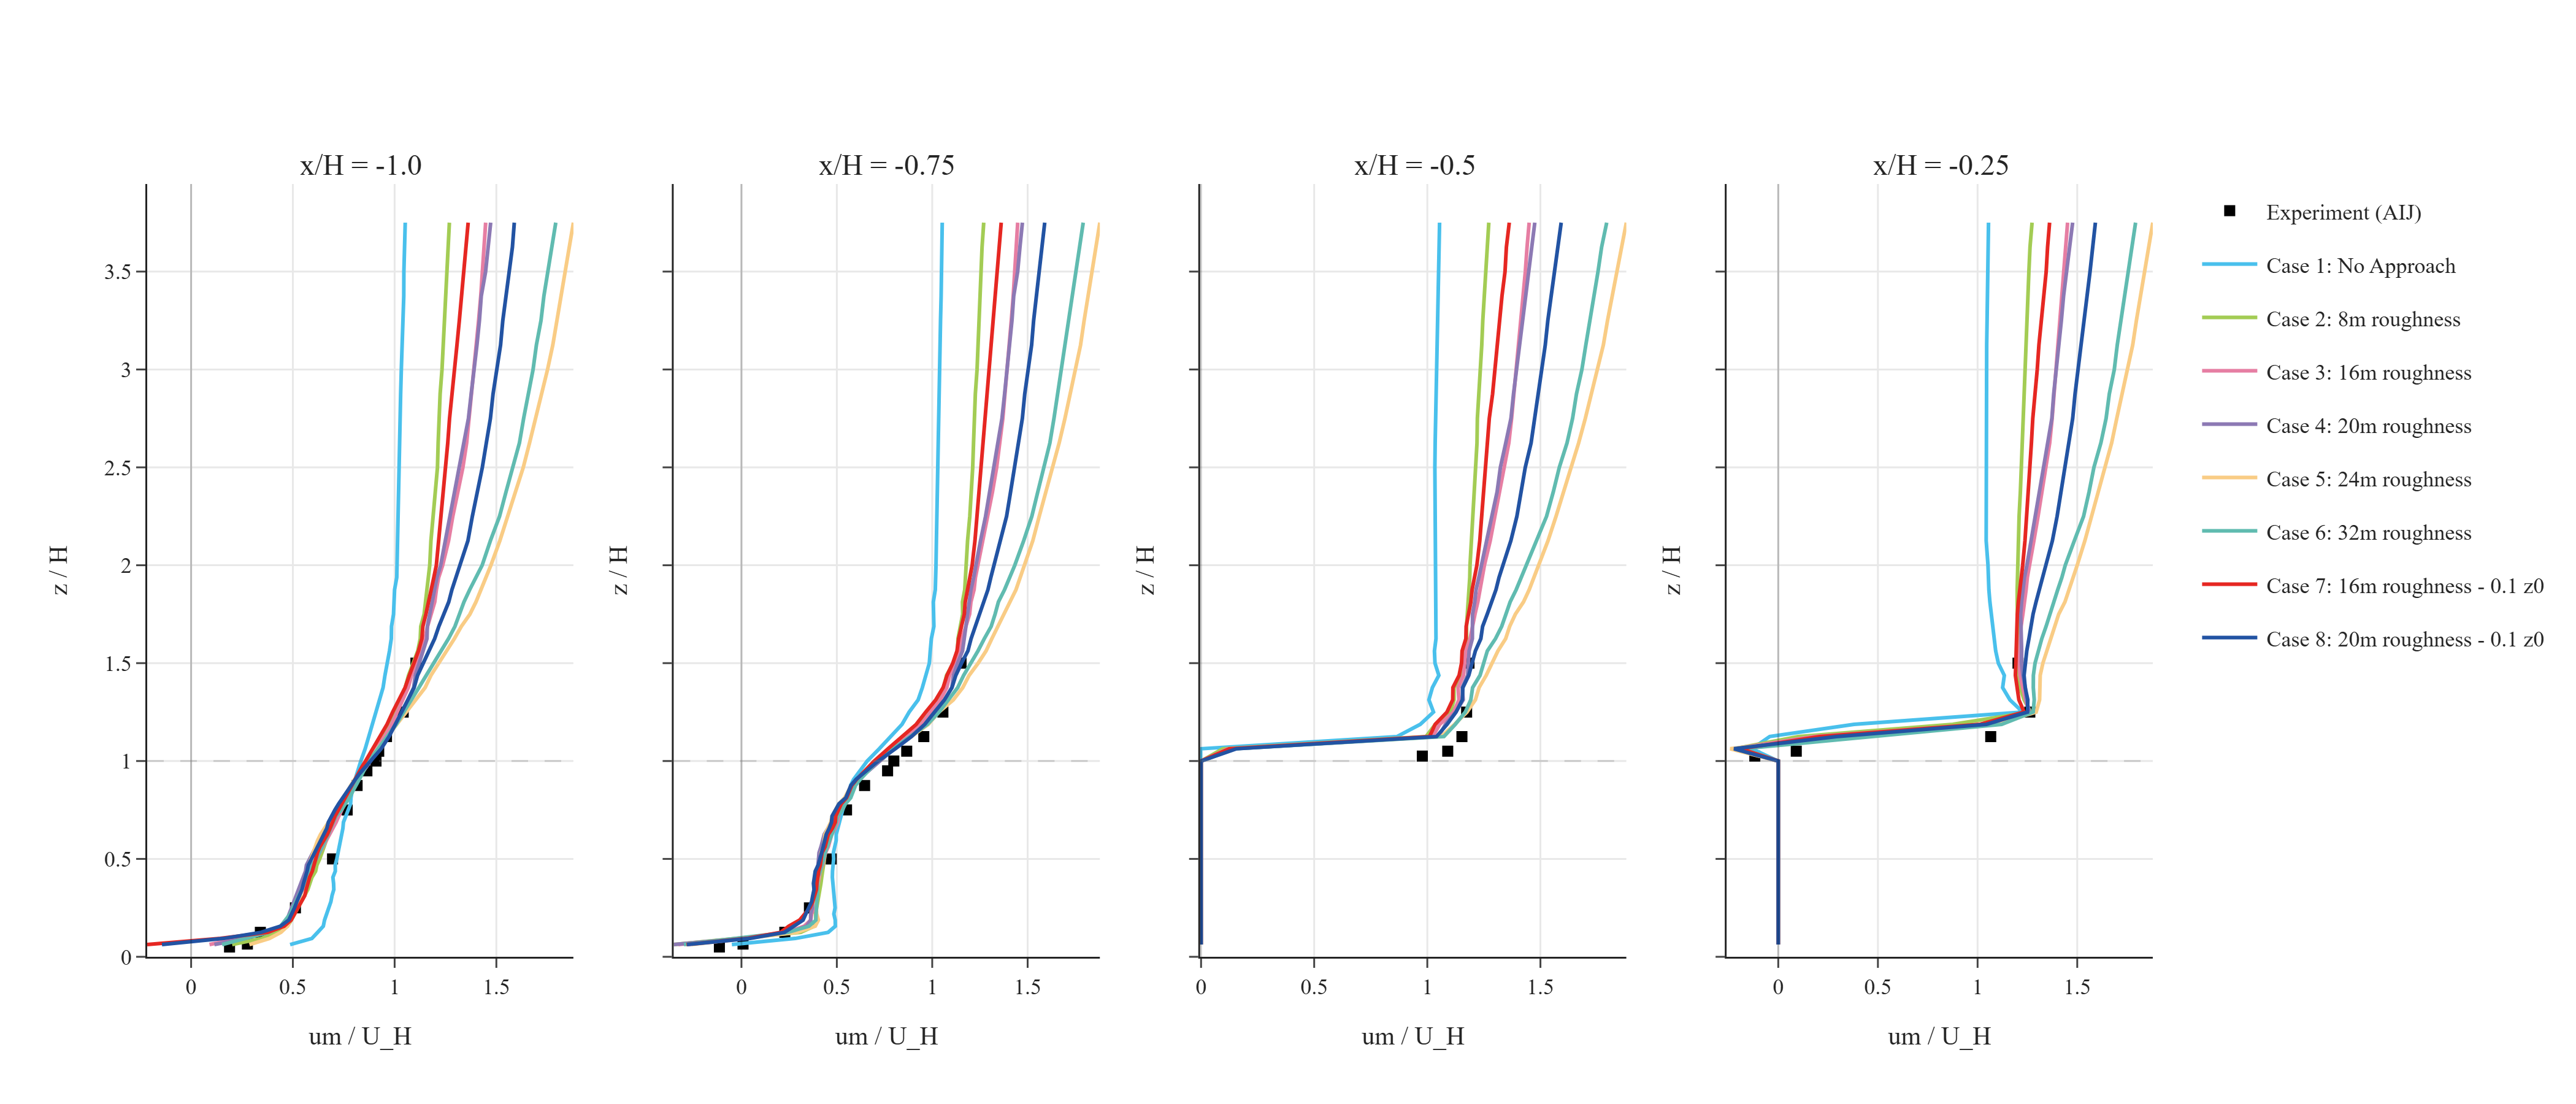
\includegraphics[width=0.85\textwidth]{figures/multi_case_comparisons_z0change/multi_case_comparison_um_part1.png}
        \caption{}
    \end{subfigure}
    \vspace{1ex}
    \begin{subfigure}[b]{\textwidth}
        \centering
        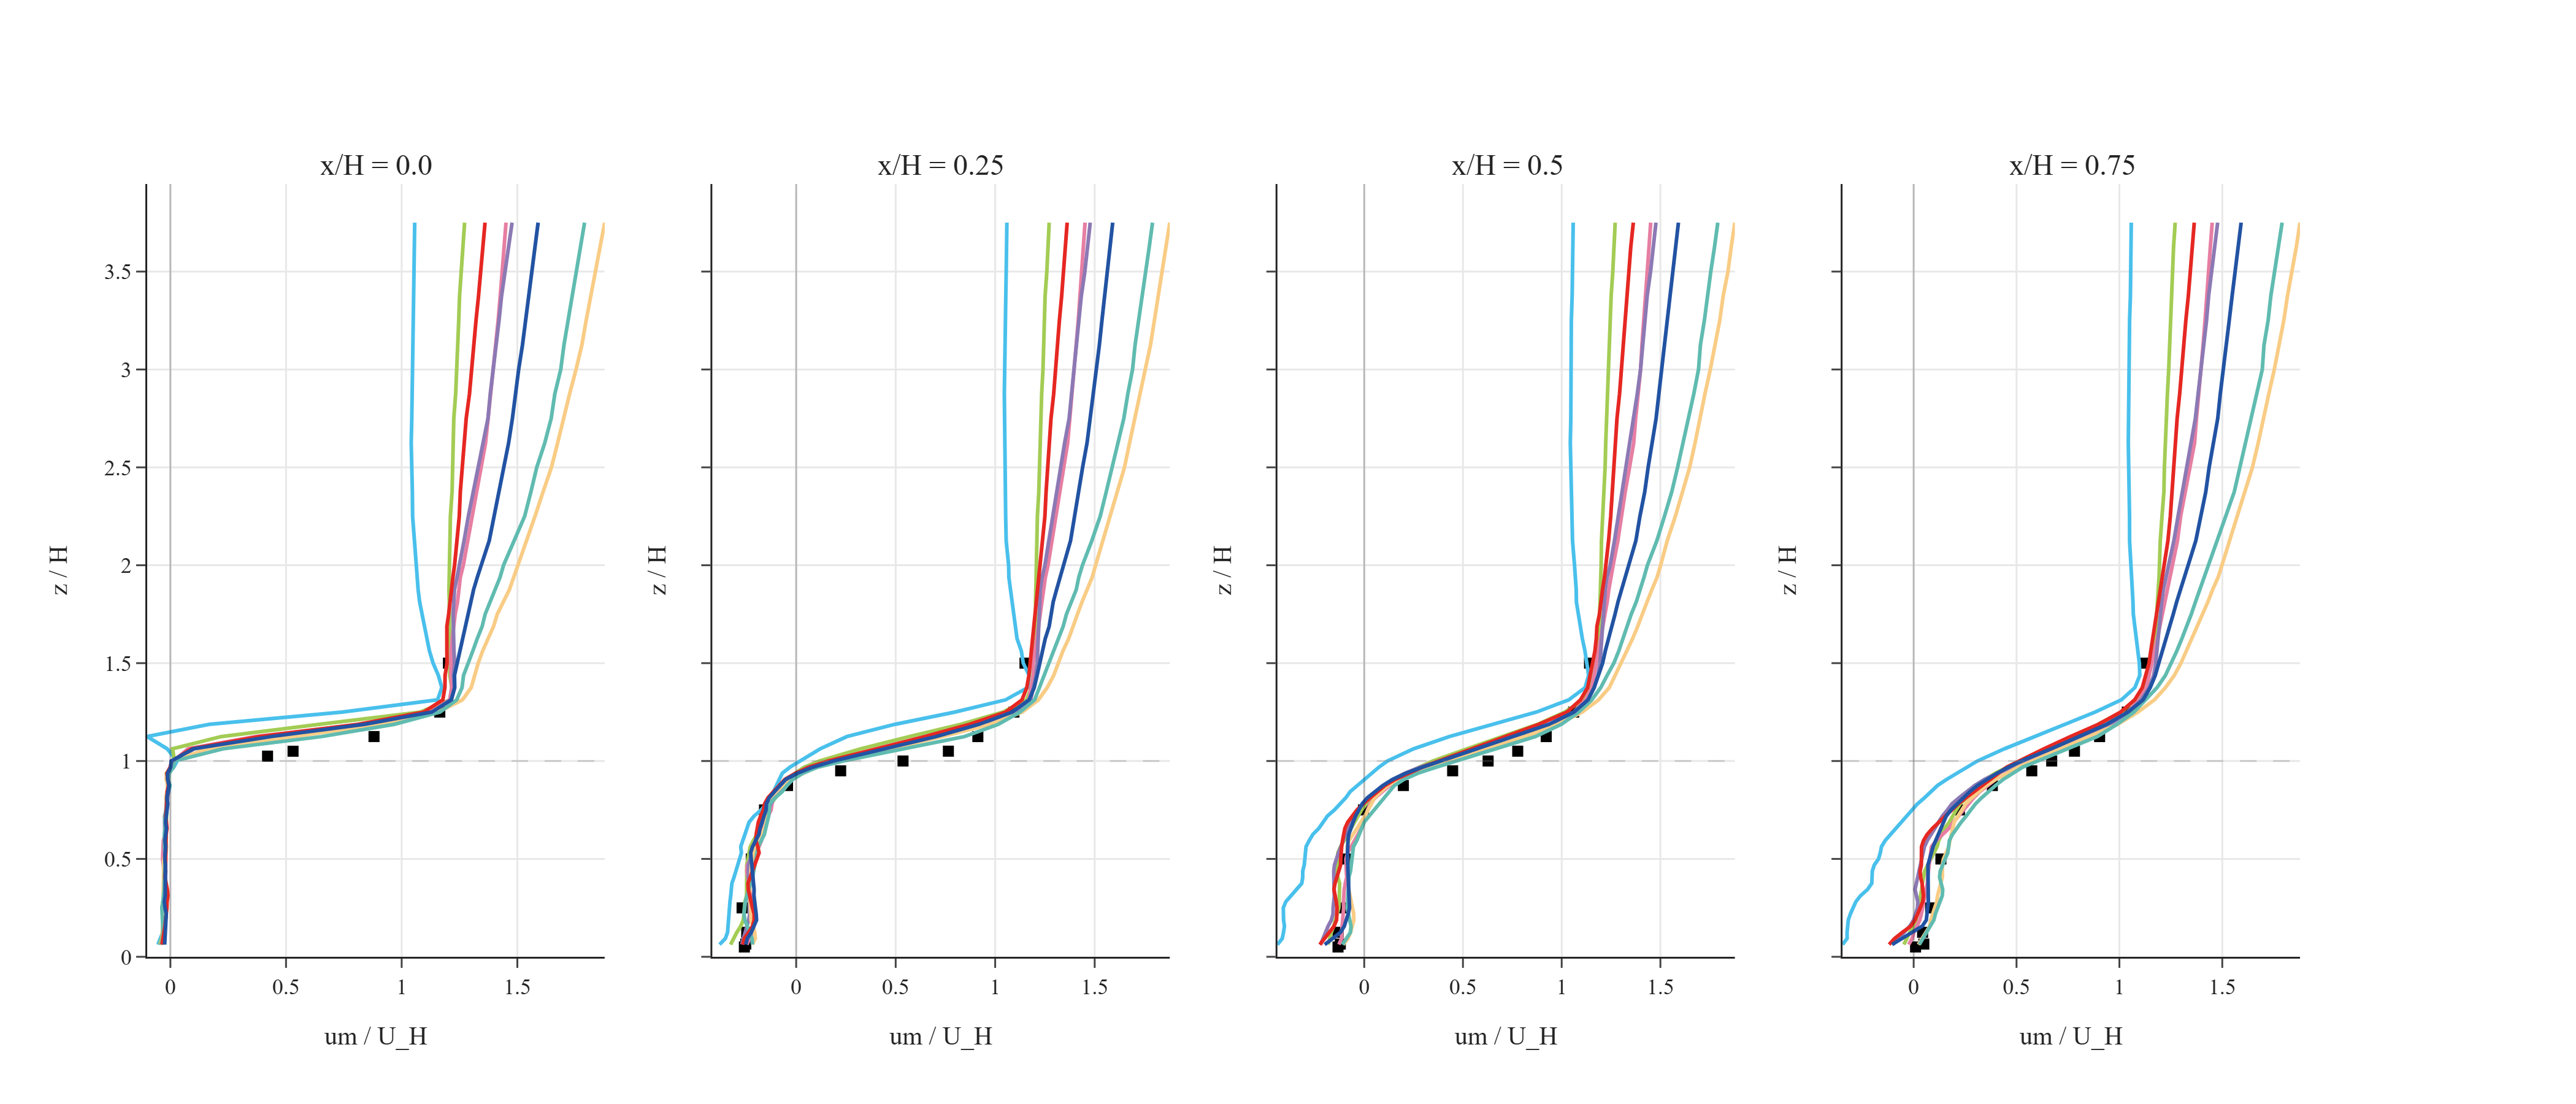
\includegraphics[width=0.85\textwidth]{figures/multi_case_comparisons_z0change/multi_case_comparison_um_part2.png}
        \caption{}
    \end{subfigure}
    \vspace{1ex}
    \begin{subfigure}[b]{\textwidth}
        \centering
        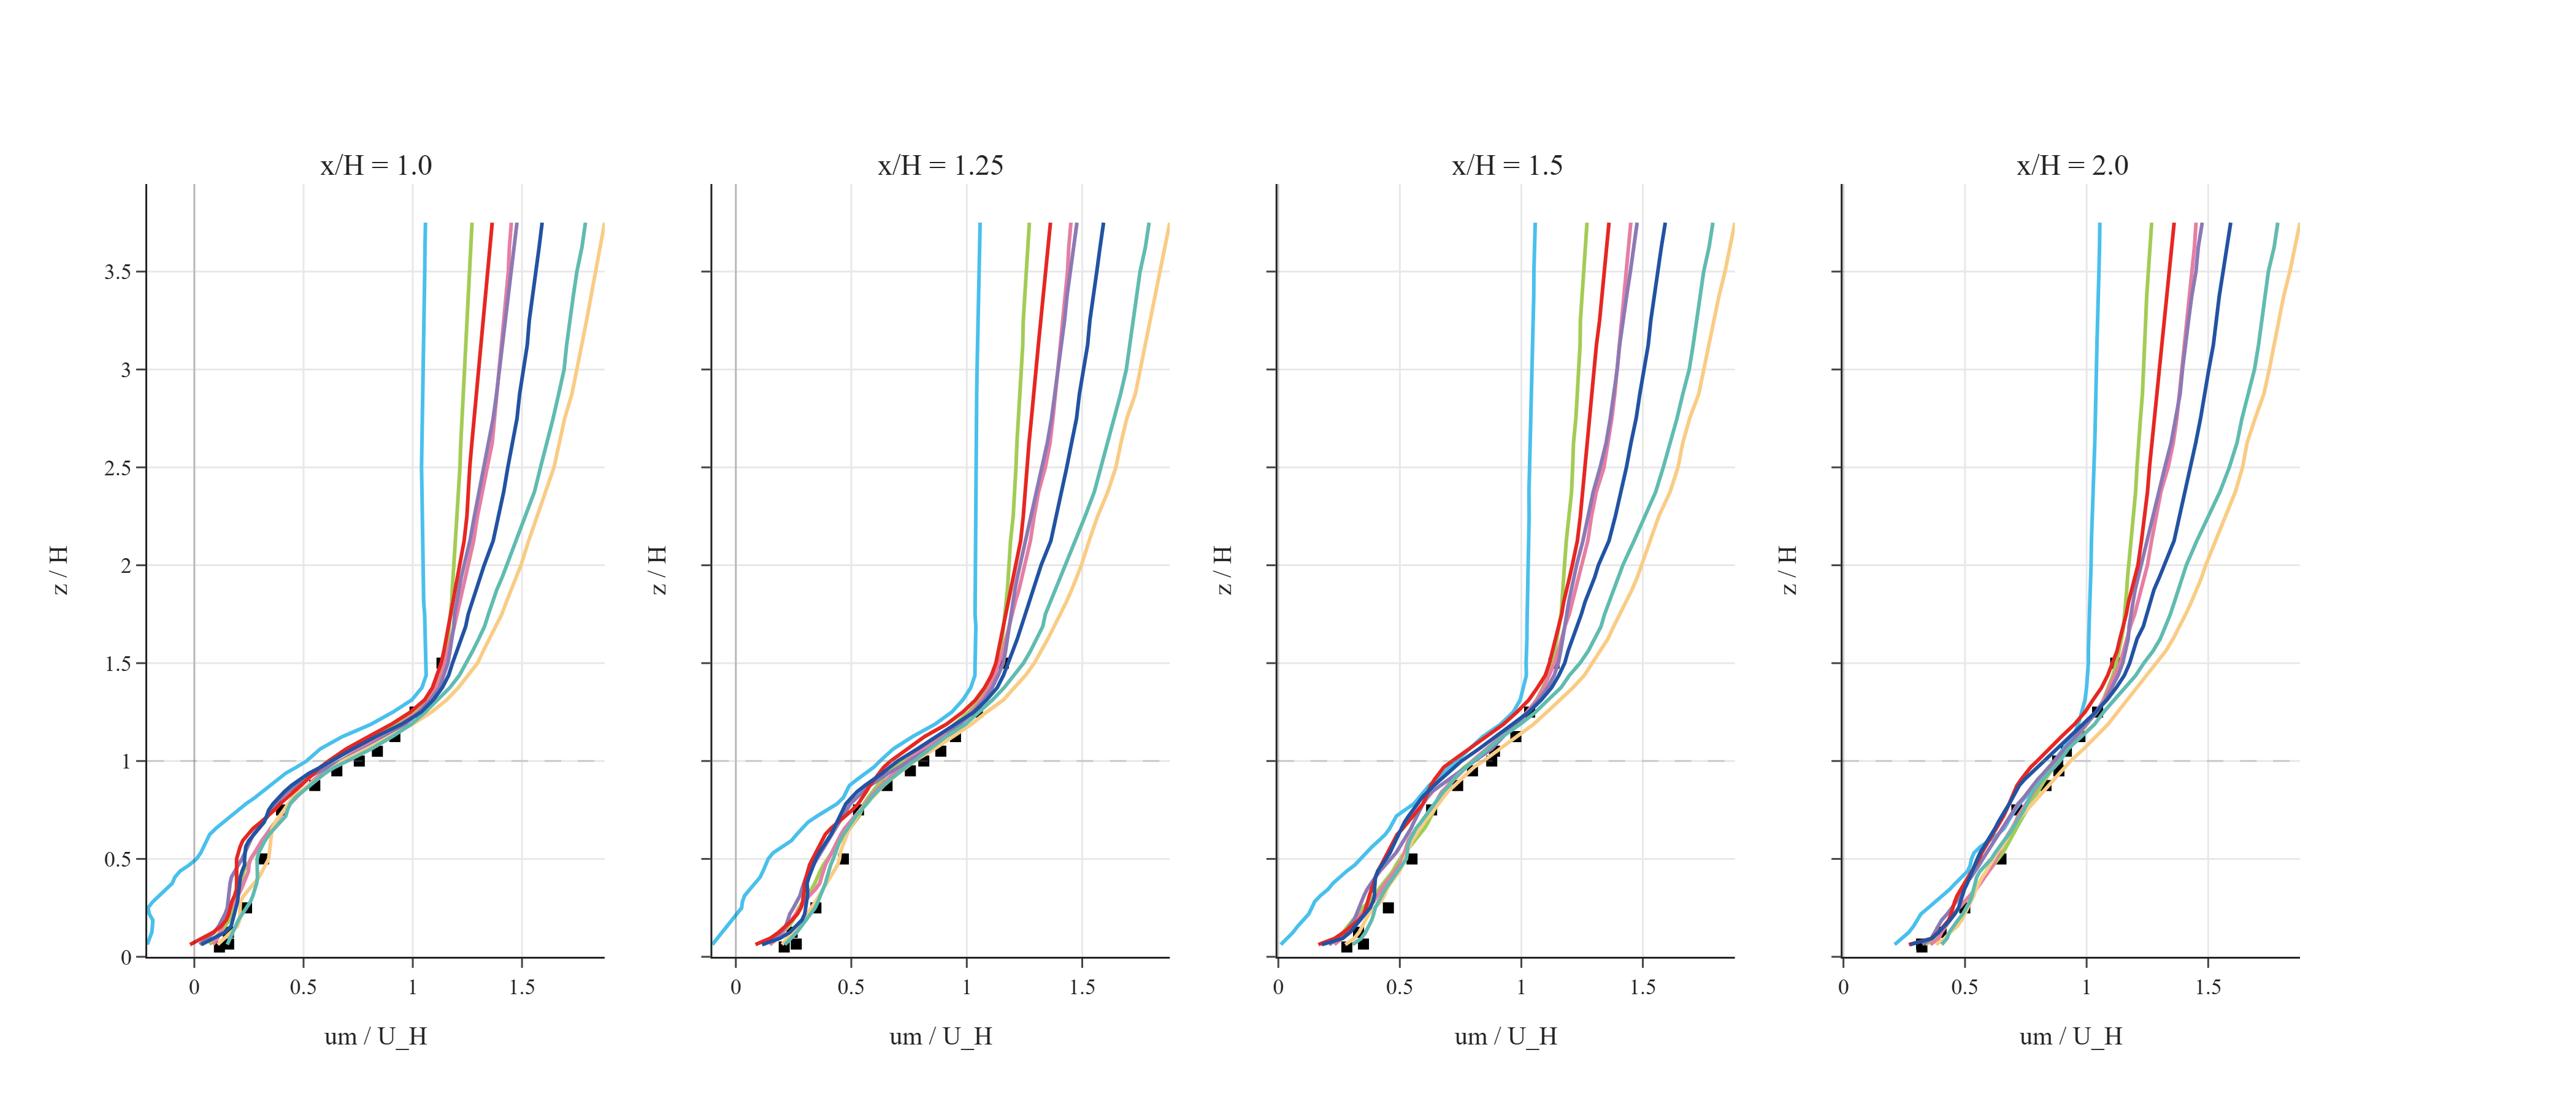
\includegraphics[width=0.85\textwidth]{figures/multi_case_comparisons_z0change/multi_case_comparison_um_part3.png}
        \caption{}
    \end{subfigure}
    \caption{Normalized mean streamwise velocity ($\bar{u}/U_H$) profiles at (a) Windward locations ($x/H = -1.0$ to $-0.25$), (b) Near Wake locations ($x/H = 0.0$ to $0.75$), and (c) Far Wake locations ($x/H = 1.0$ to $2.0$).}
    \label{fig:results_um}
\end{figure}

\autoref{fig:results_um} illustrates the vertical profiles of the normalized streamwise velocity ($u/U_H$) at the locations defined in \autoref{fig:measurement_points}. A primary observation is that the simulation's ability to reproduce the experimental data improves significantly as the inflow turbulence increases, driven by the added roughness in the approach section. Even in the most simplified cases lacking approach roughness, the LBM results maintain the general characteristic shape observed in the AIJ wind tunnel experiments, capturing the fundamental flow deceleration and wake recovery. However, the introduction of even minimal roughness provides a substantial increase in accuracy, effectively closing the gap between the numerical and experimental data. Beyond this initial improvement, the profiles exhibit a plateau in refinement; the variation between different high-roughness cases is minimal, suggesting that once the atmospheric boundary layer is sufficiently developed, the broad-scale structure of the streamwise velocity becomes stable. This indicates that the presence of upstream turbulence is more critical for profile accuracy than the specific magnitude of the roughness height once a certain threshold is reached.

% --- Mean Spanwise Velocity (v) ---
\begin{figure}[htbp]
    \centering
    \begin{subfigure}[b]{\textwidth}
        \centering
        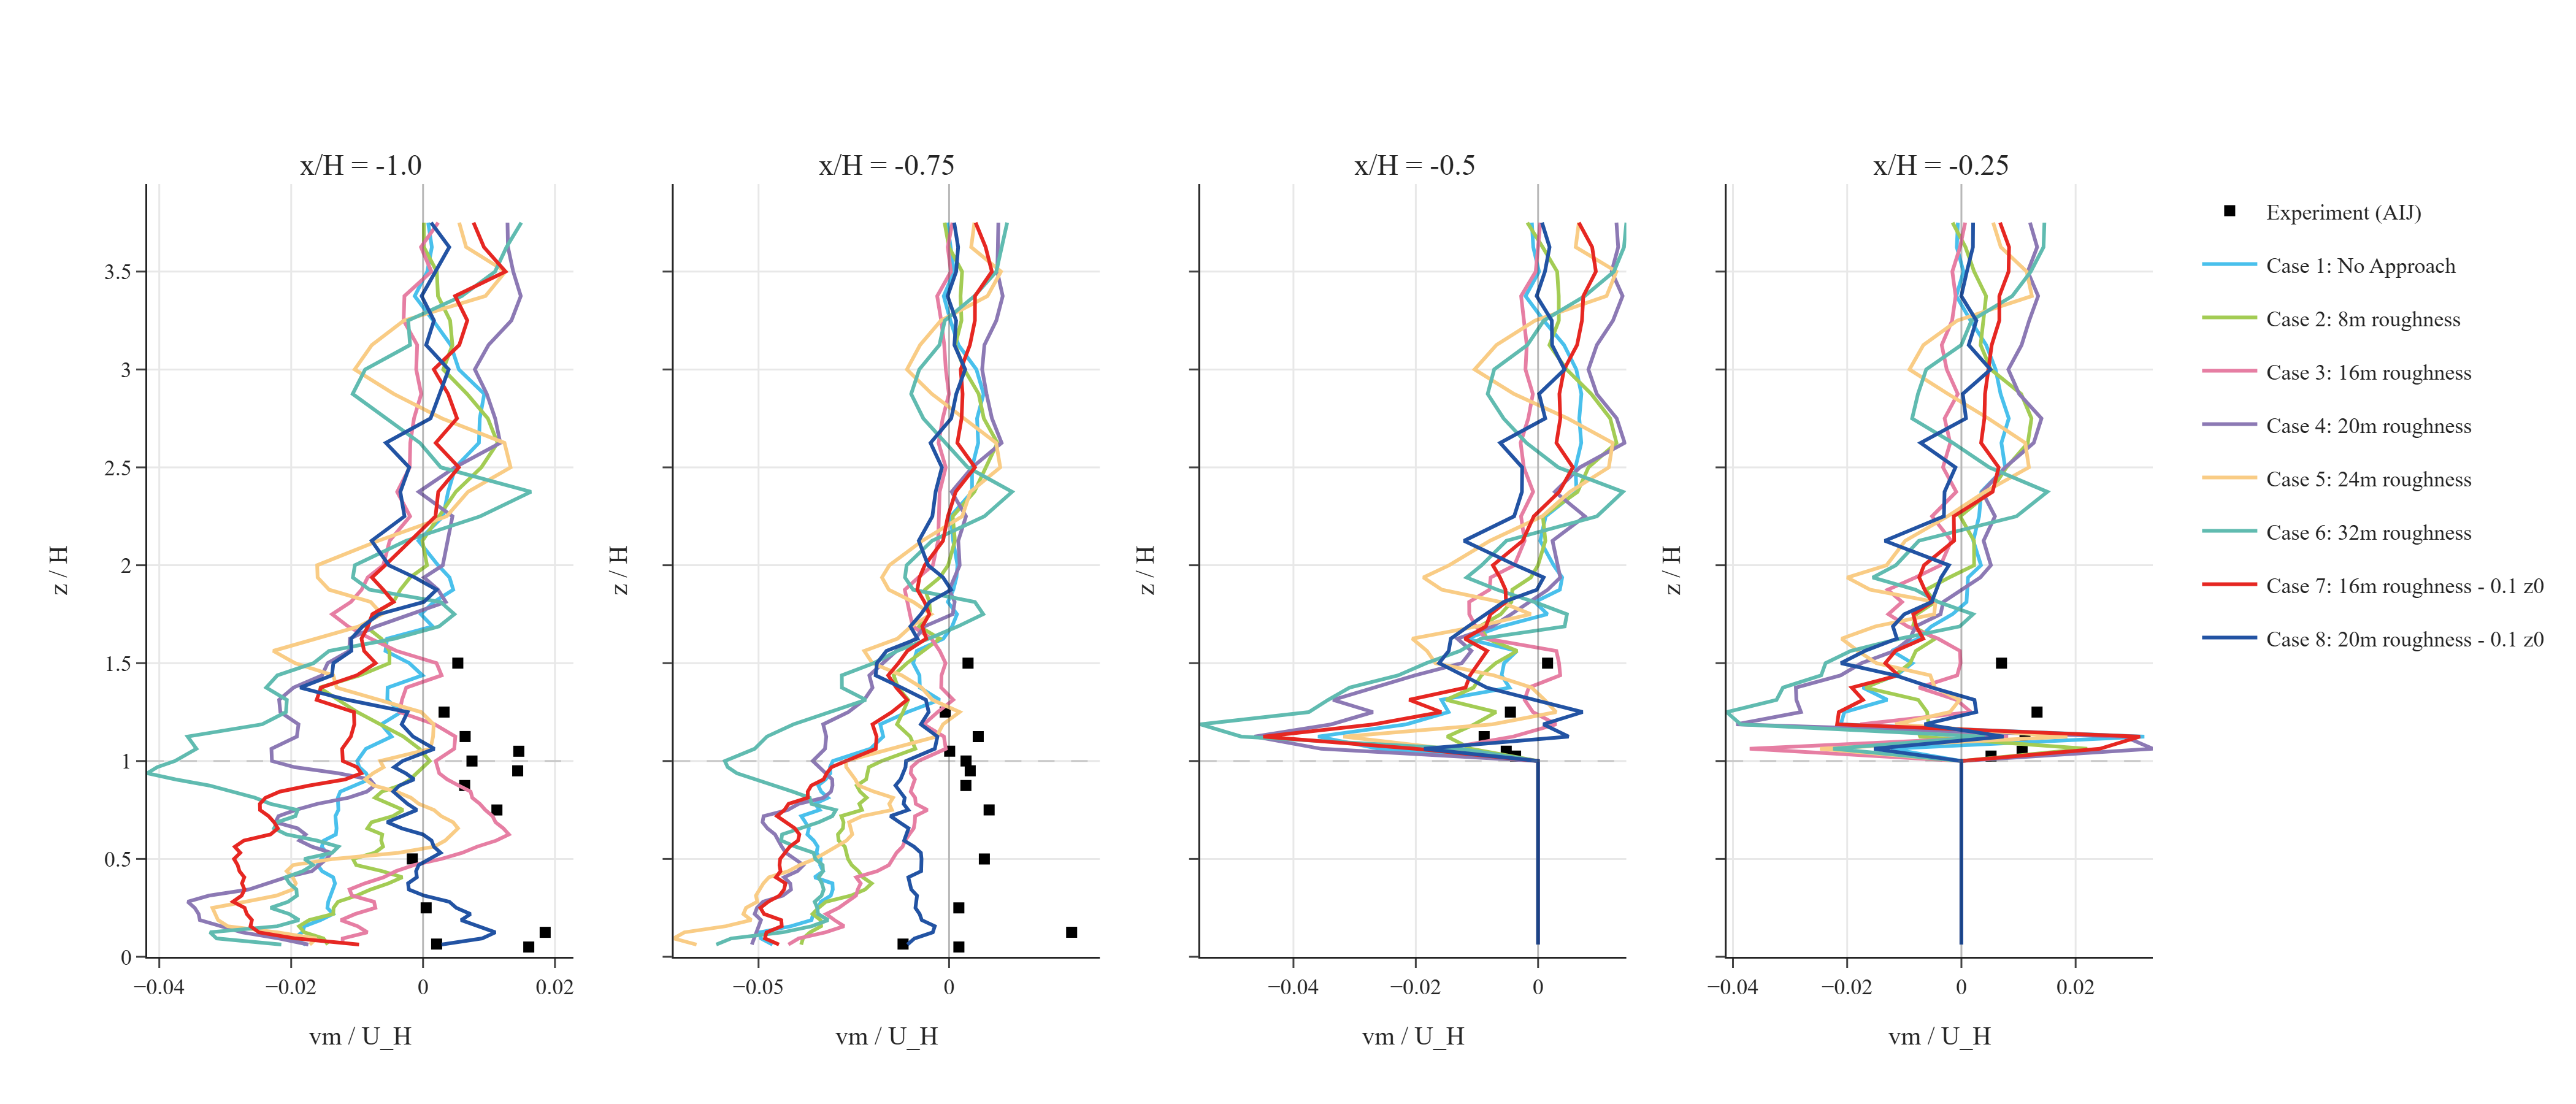
\includegraphics[width=0.85\textwidth]{figures/multi_case_comparisons_z0change/multi_case_comparison_vm_part1.png}
        \caption{}
    \end{subfigure}
    \vspace{1ex}
    \begin{subfigure}[b]{\textwidth}
        \centering
        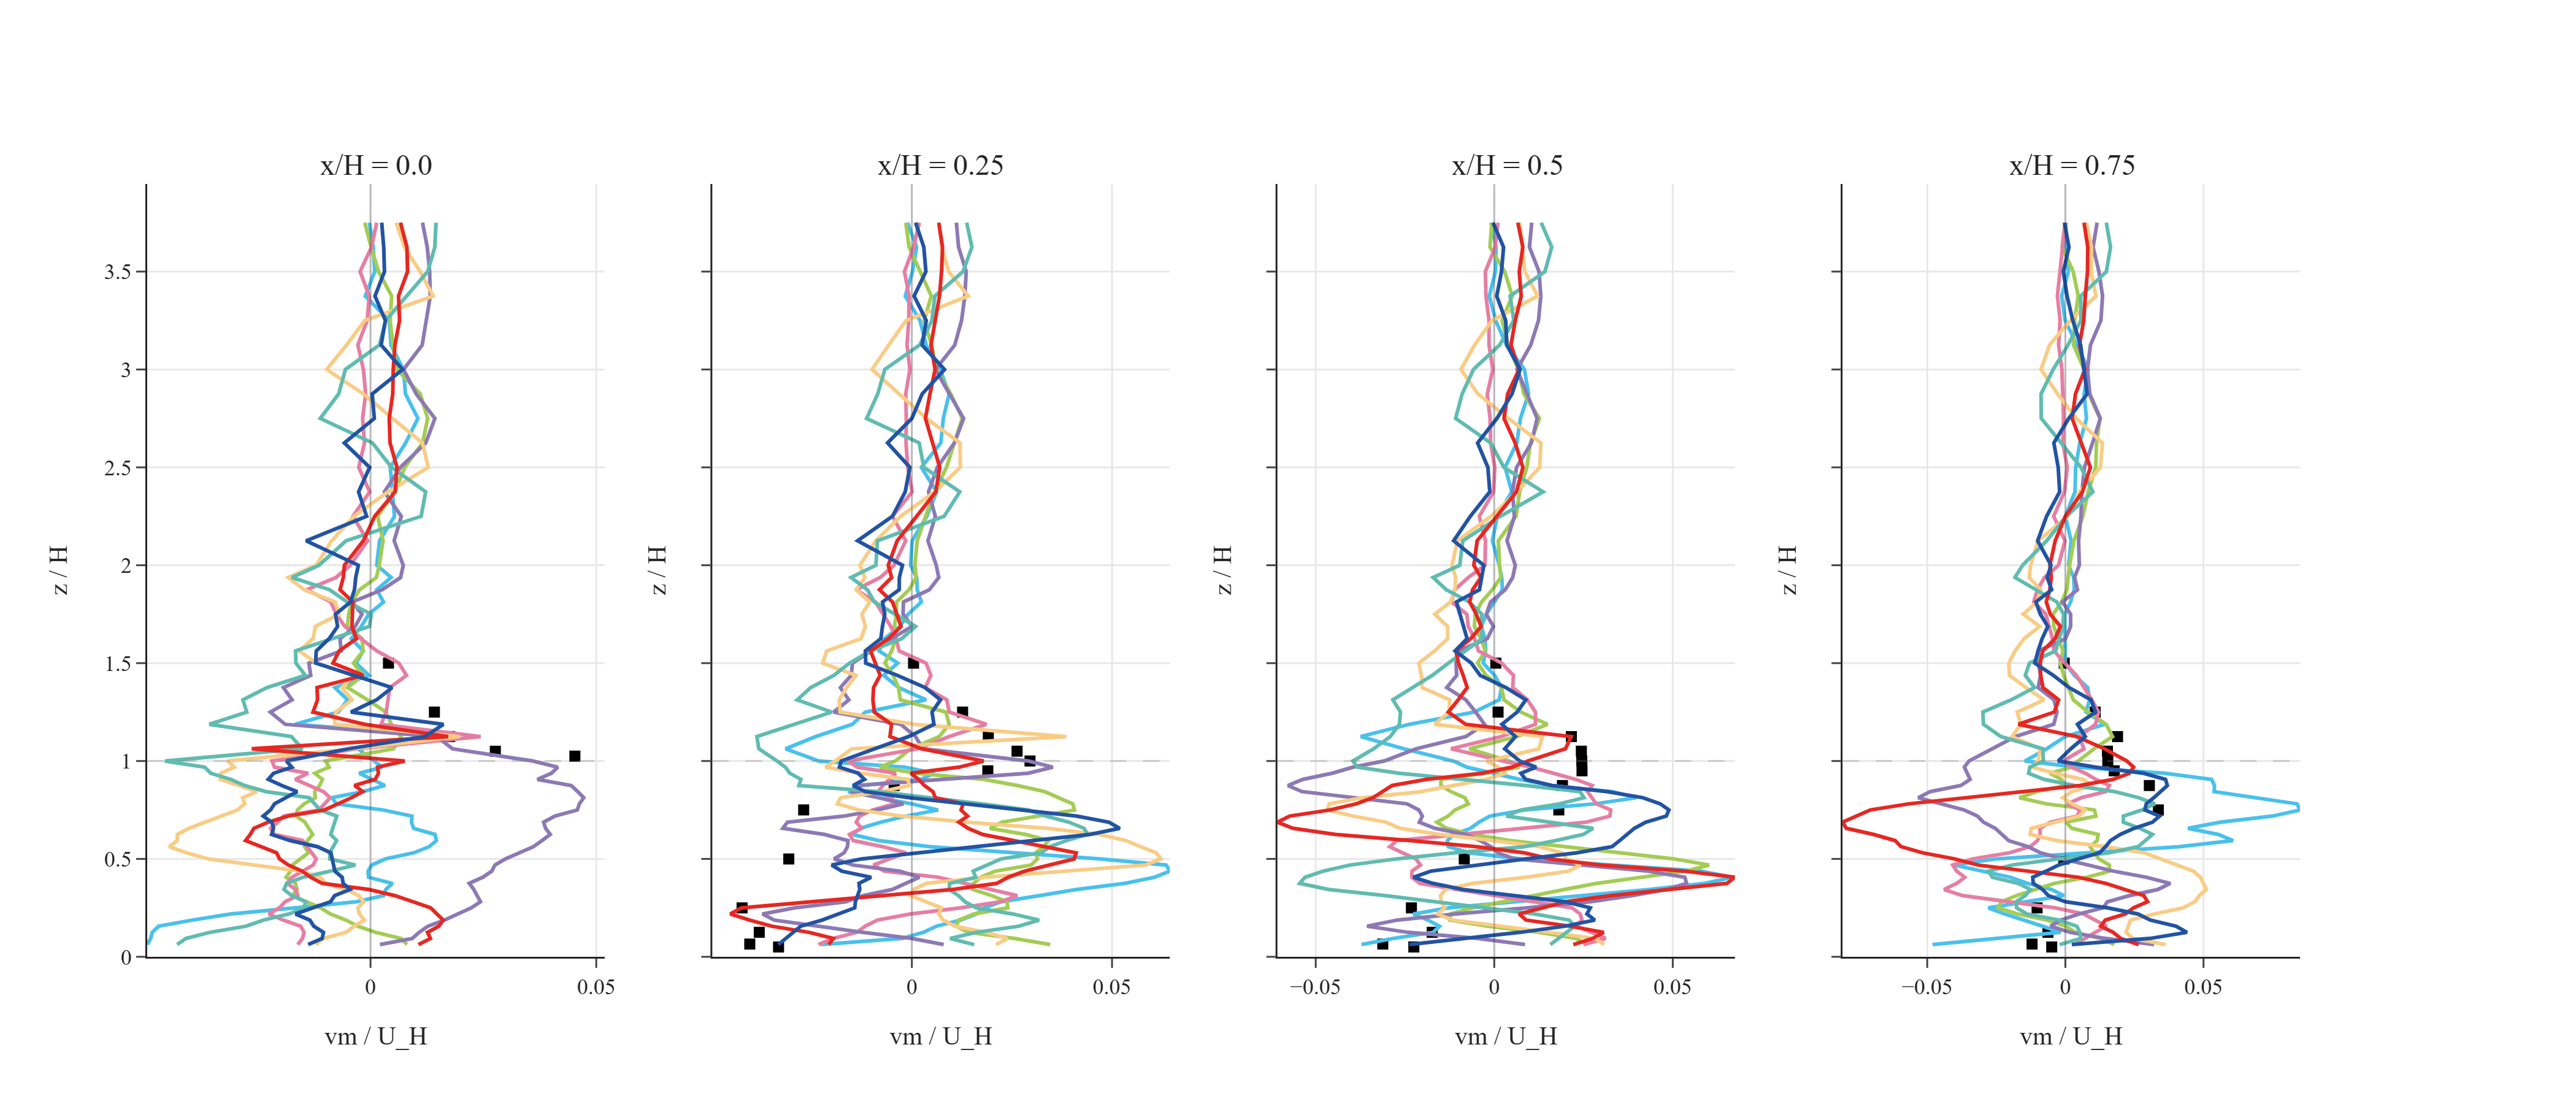
\includegraphics[width=0.85\textwidth]{figures/multi_case_comparisons_z0change/multi_case_comparison_vm_part2.png}
        \caption{}
    \end{subfigure}
    \vspace{1ex}
    \begin{subfigure}[b]{\textwidth}
        \centering
        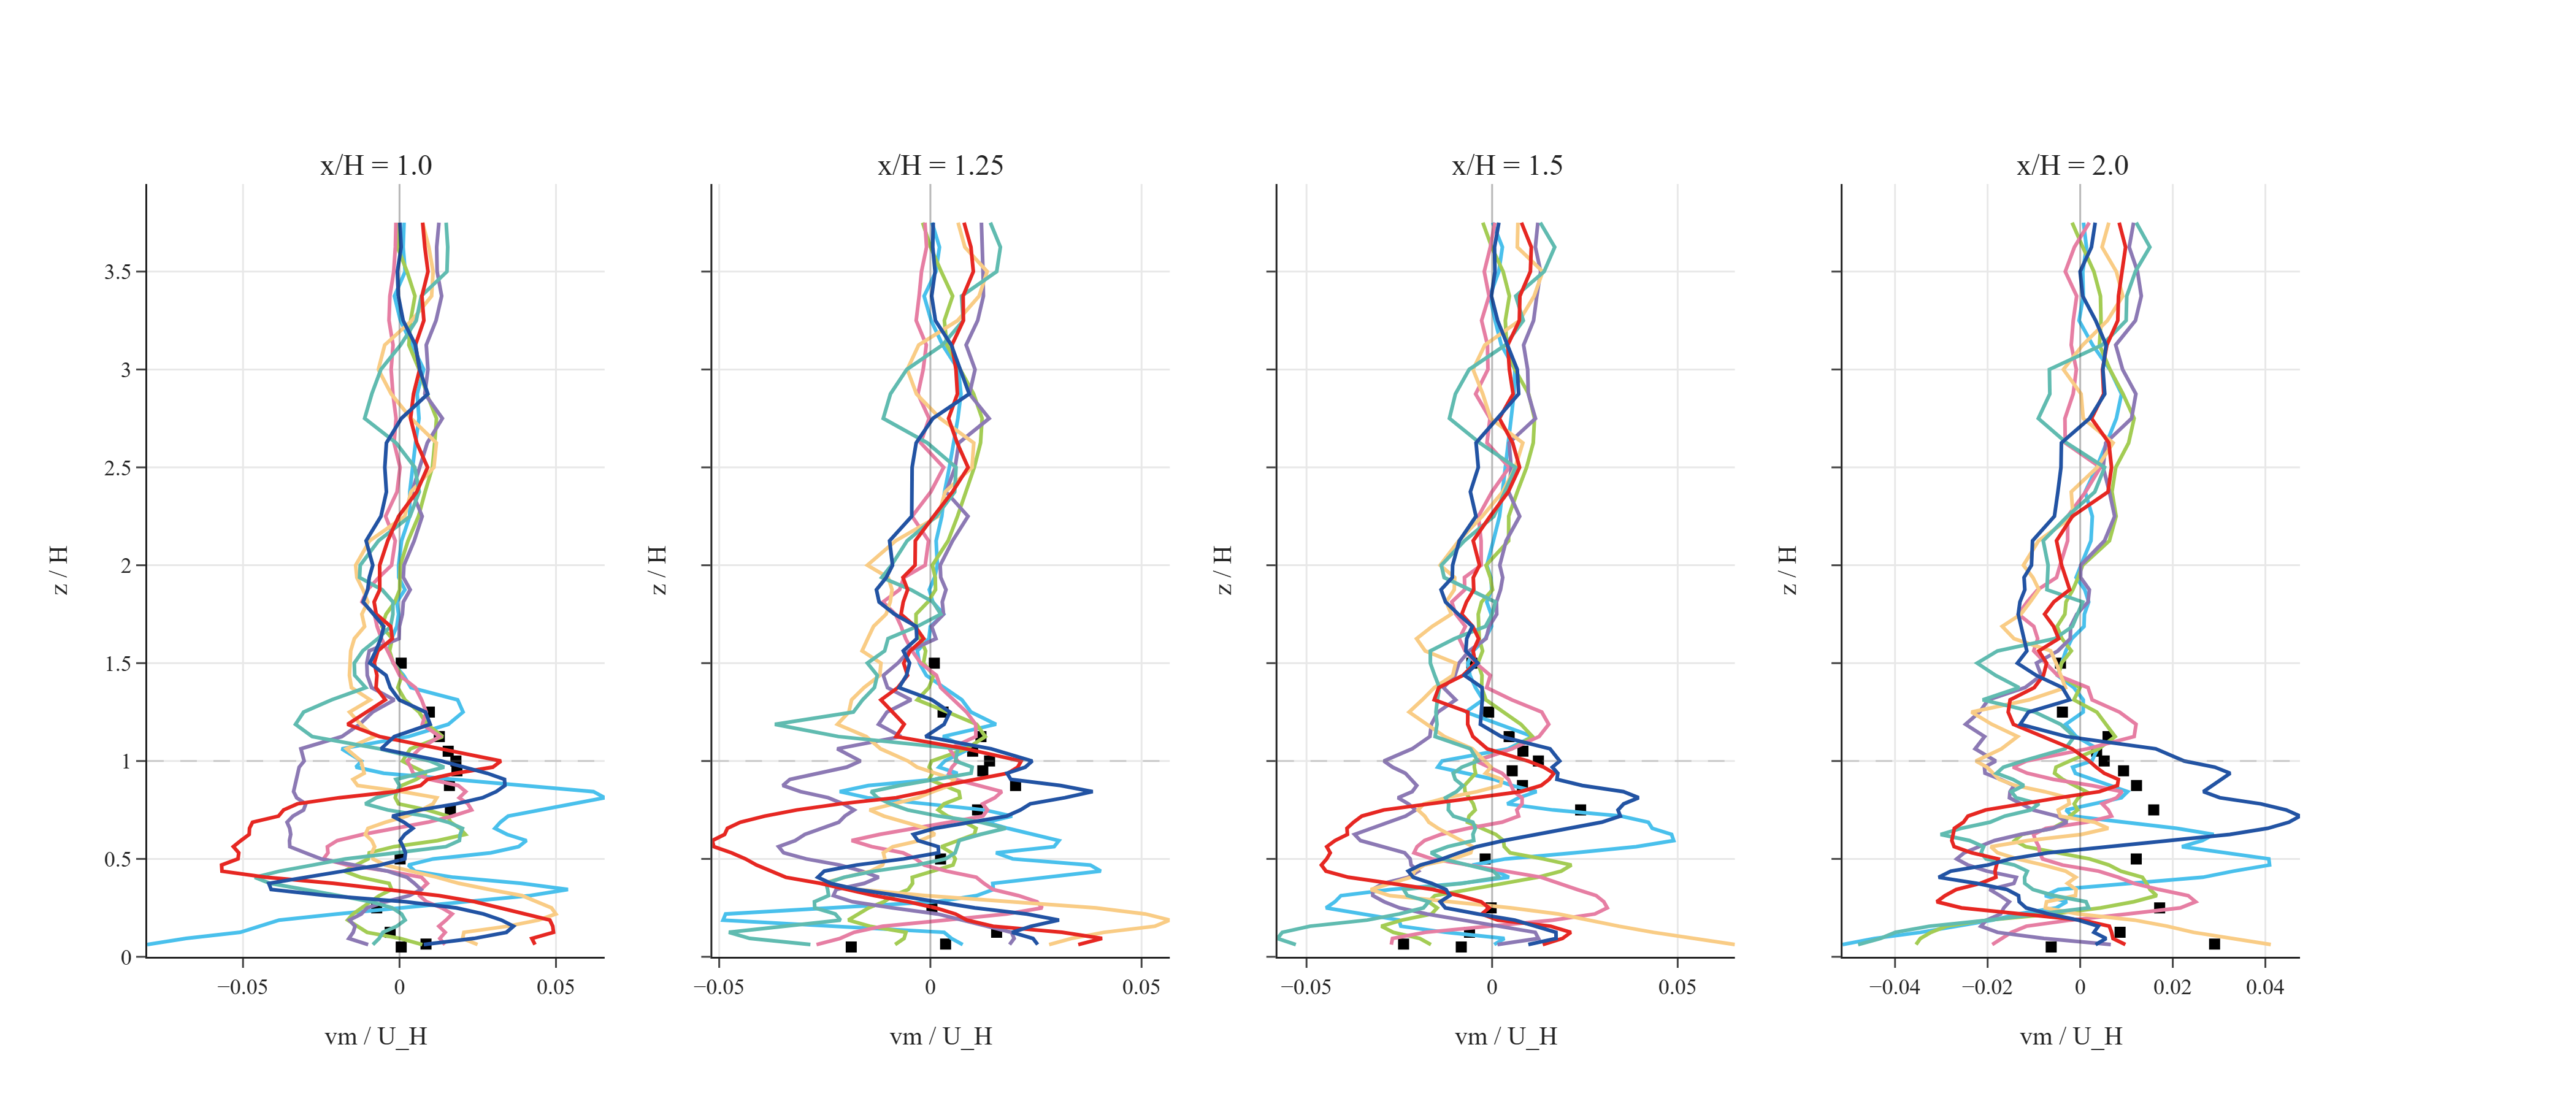
\includegraphics[width=0.85\textwidth]{figures/multi_case_comparisons_z0change/multi_case_comparison_vm_part3.png}
        \caption{}
    \end{subfigure}
    \caption{Normalized mean spanwise velocity ($\bar{v}/U_H$) profiles at (a) $x/H = -1.0$ to $-0.25$, (b) $x/H = 0.0$ to $0.75$, and (c) $x/H = 1.0$ to $2.0$.}
    \label{fig:results_vm}
\end{figure}

\autoref{fig:results_vm} presents the vertical profiles of the normalized spanwise velocity ($v/U_H$). In contrast to the streamwise results, the spanwise profiles are largely inconclusive regarding the impact of approach roughness. Both the experimental data and numerical results exhibit small-scale fluctuations with magnitudes on the order of $10^{-2}$, representing minor lateral shifts in the wind direction. Due to the stochastic nature of these lateral movements and their negligible magnitude relative to the primary flow, the patterns appear relatively random. Consequently, no significant correlation can be established between the increase in upstream turbulence and the predictive accuracy of the spanwise velocity component in the near-field wake.

% --- Mean Vertical Velocity (w) ---
\begin{figure}[htbp]
    \centering
    \begin{subfigure}[b]{\textwidth}
        \centering
        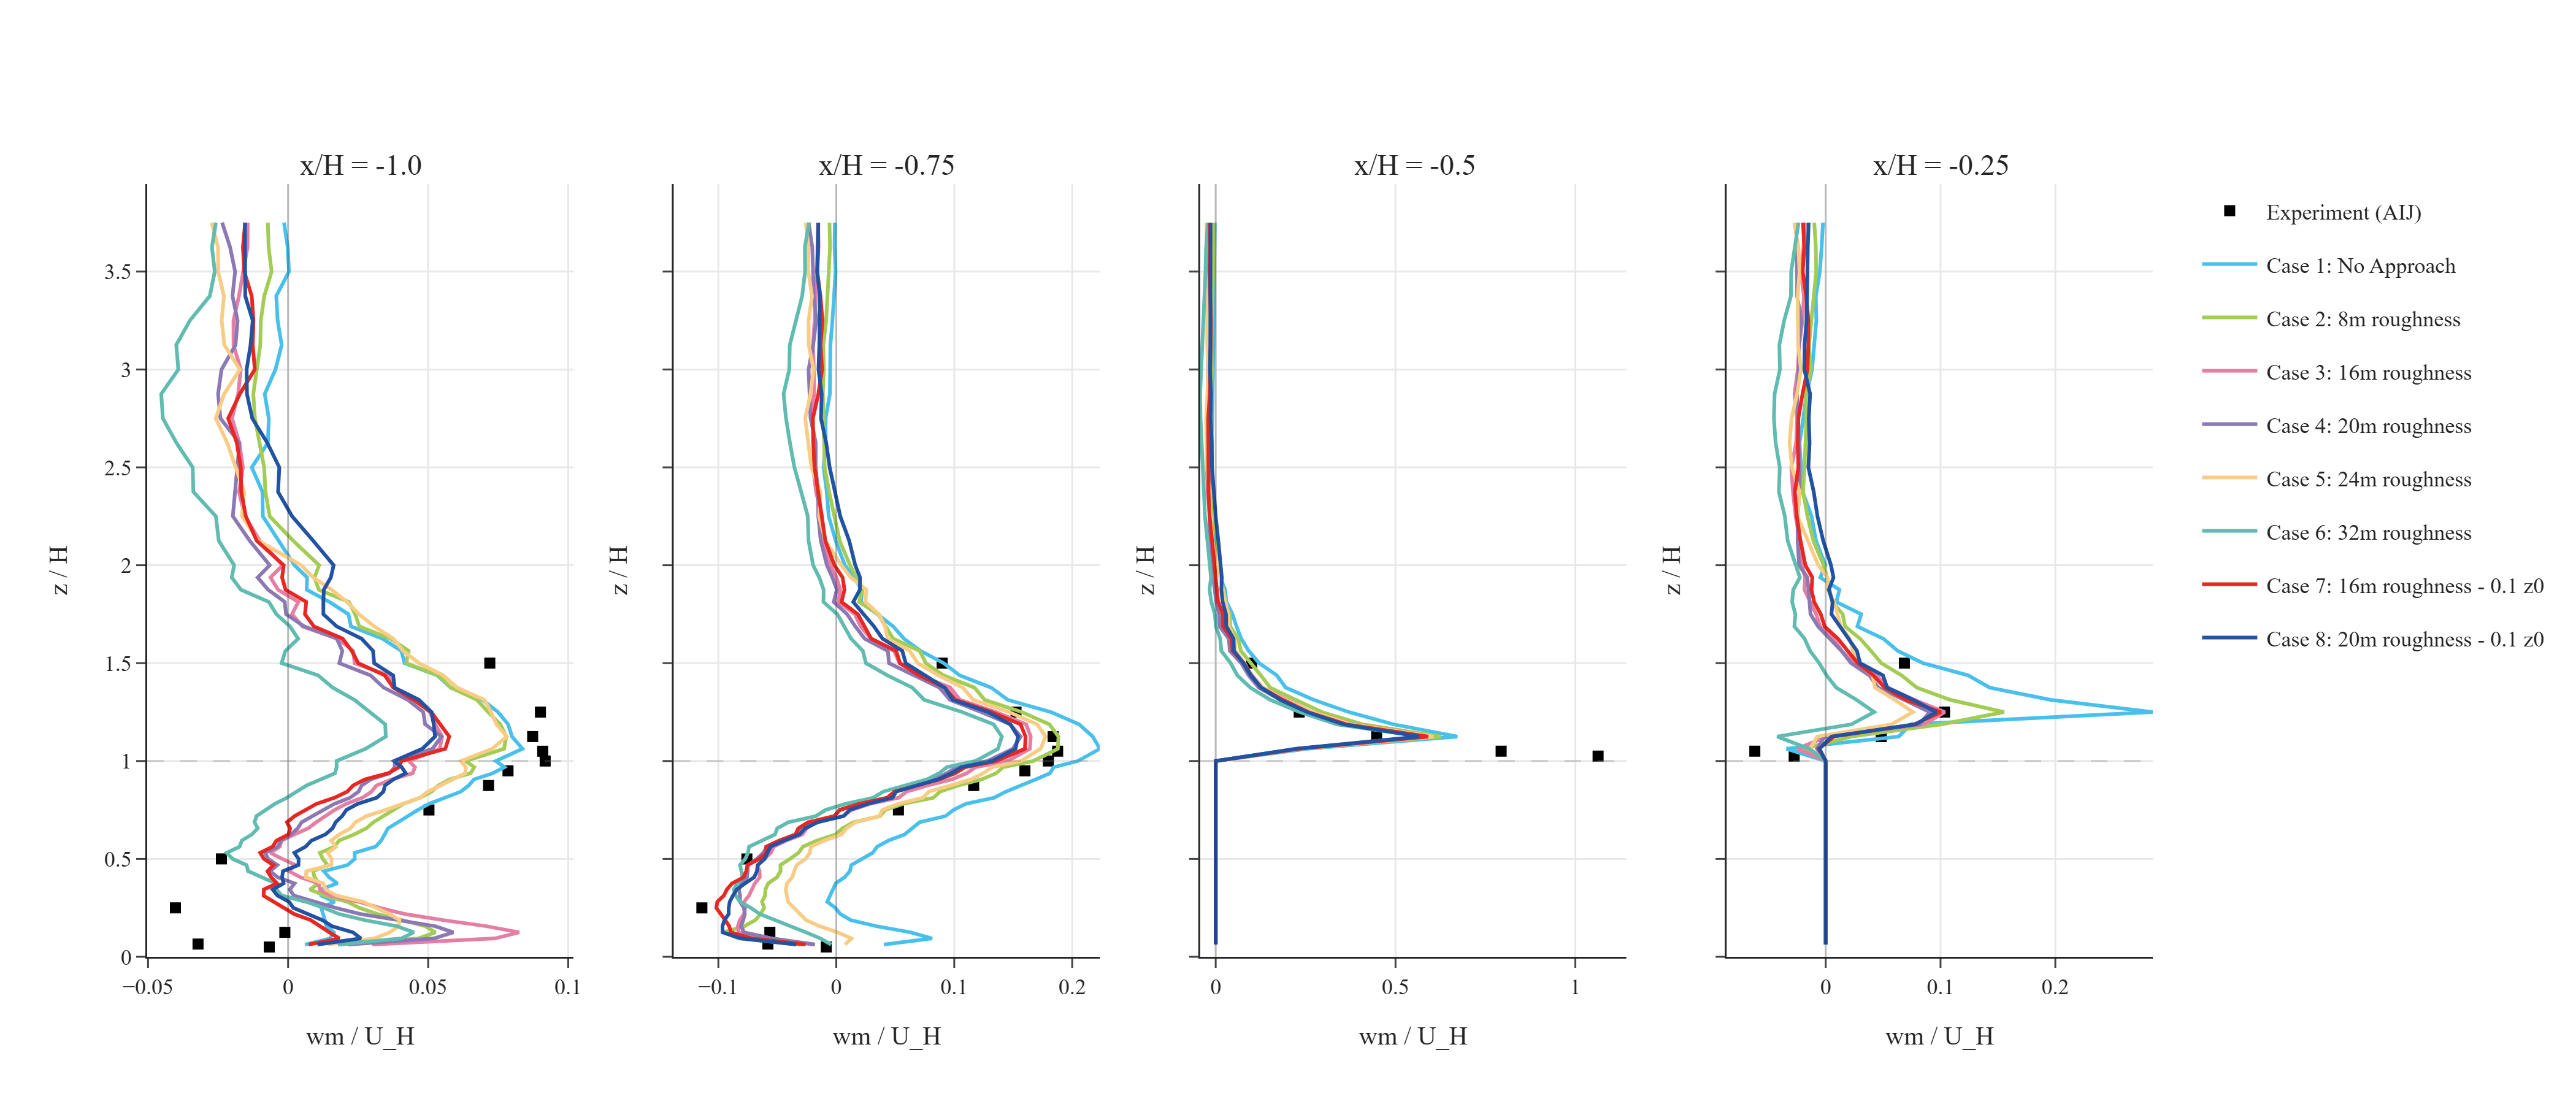
\includegraphics[width=0.85\textwidth]{figures/multi_case_comparisons_z0change/multi_case_comparison_wm_part1.png}
        \caption{}
    \end{subfigure}
    \vspace{1ex}
    \begin{subfigure}[b]{\textwidth}
        \centering
        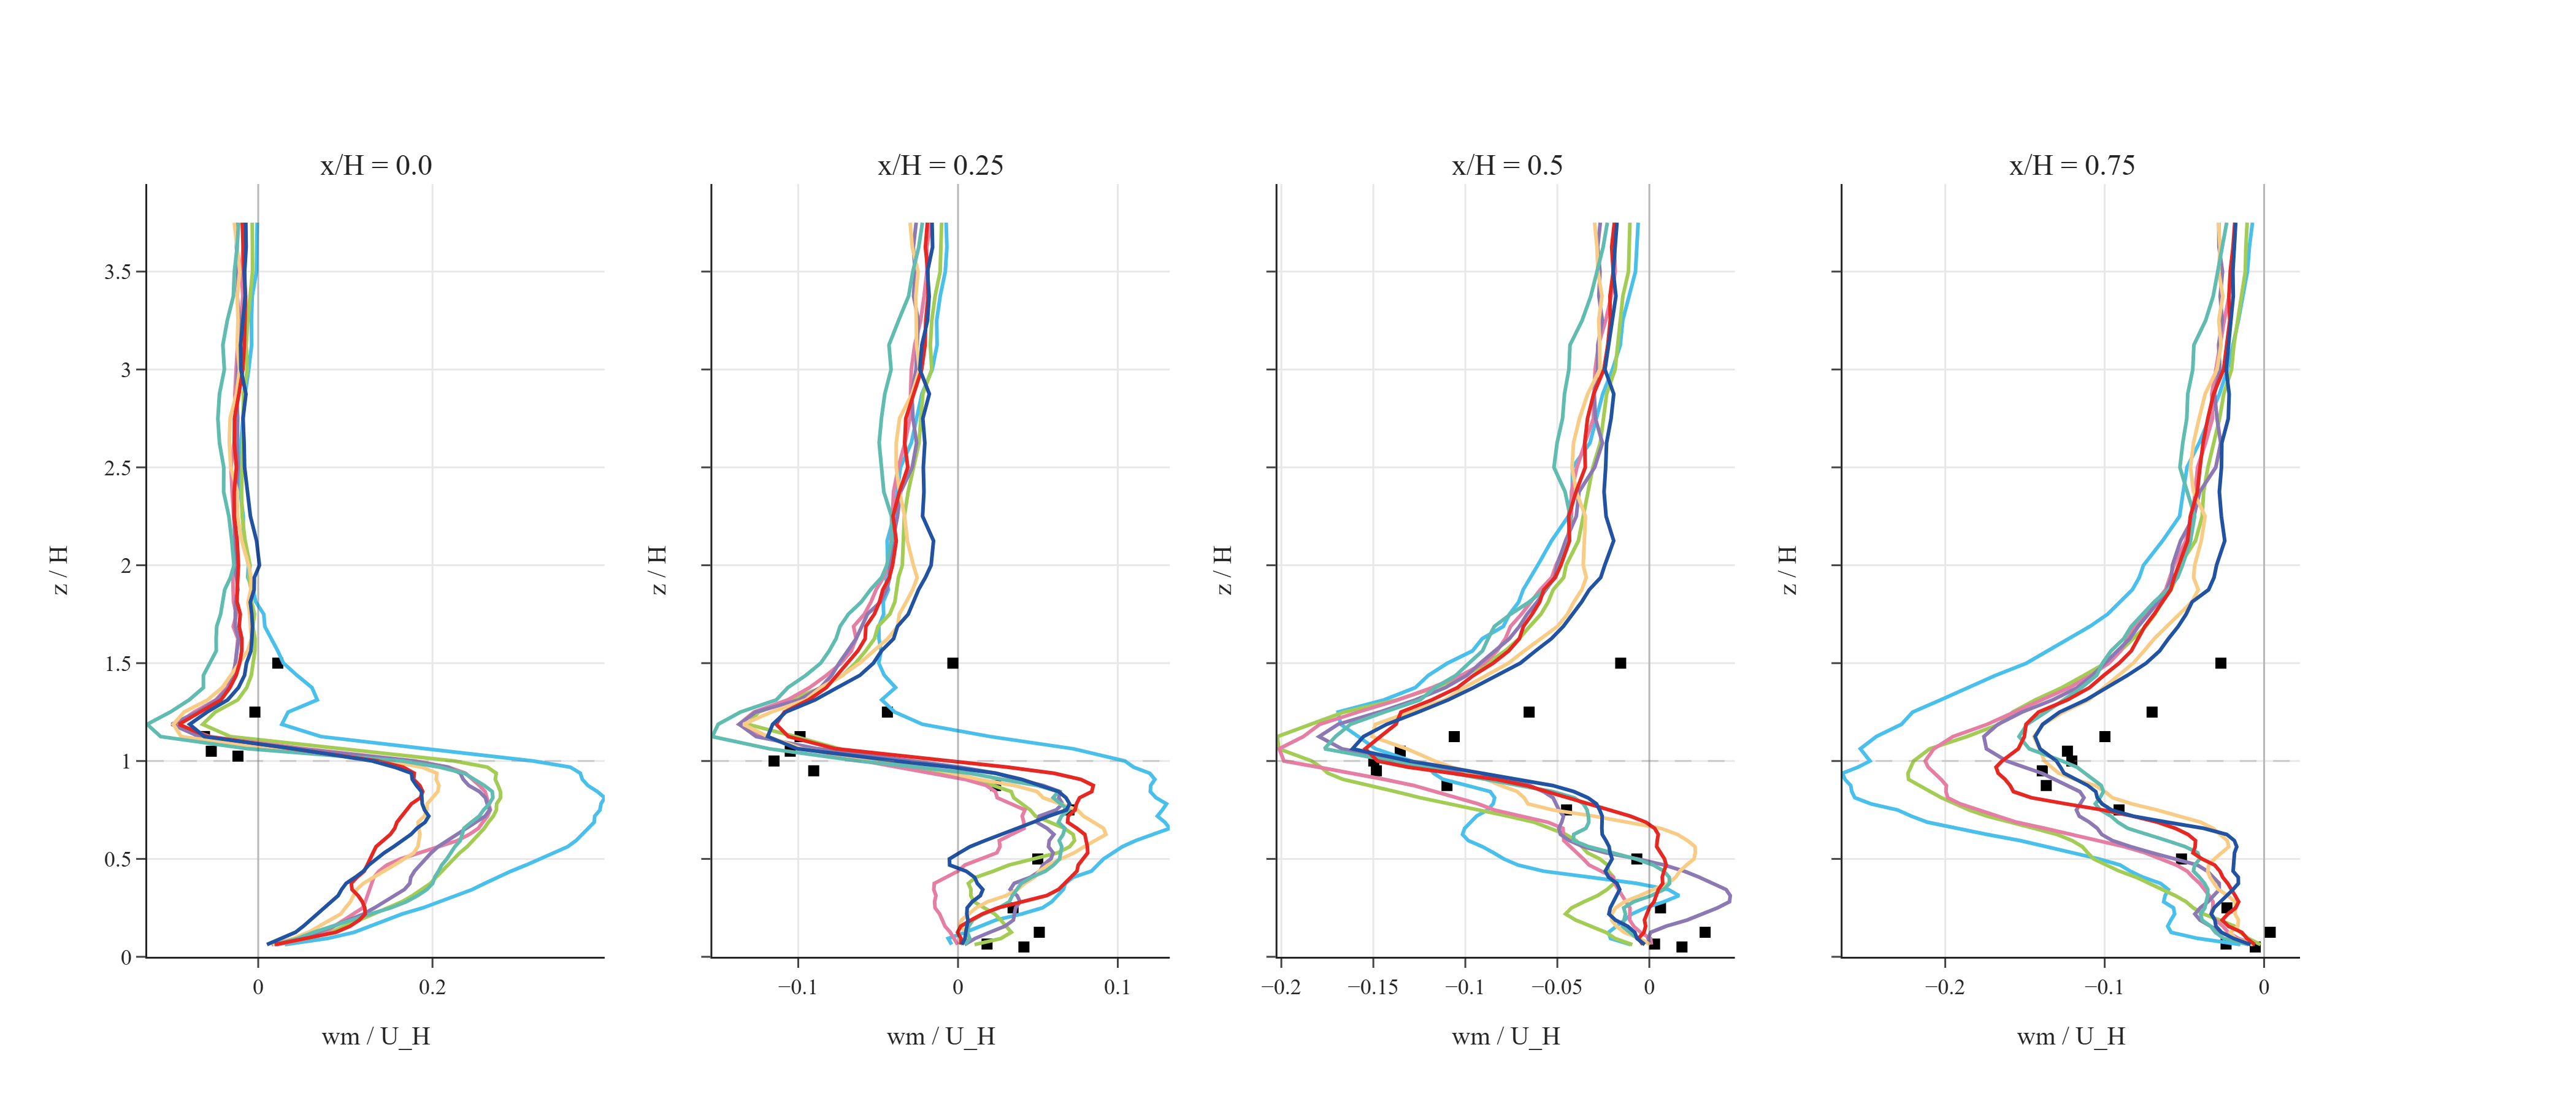
\includegraphics[width=0.85\textwidth]{figures/multi_case_comparisons_z0change/multi_case_comparison_wm_part2.png}
        \caption{}
    \end{subfigure}
    \vspace{1ex}
    \begin{subfigure}[b]{\textwidth}
        \centering
        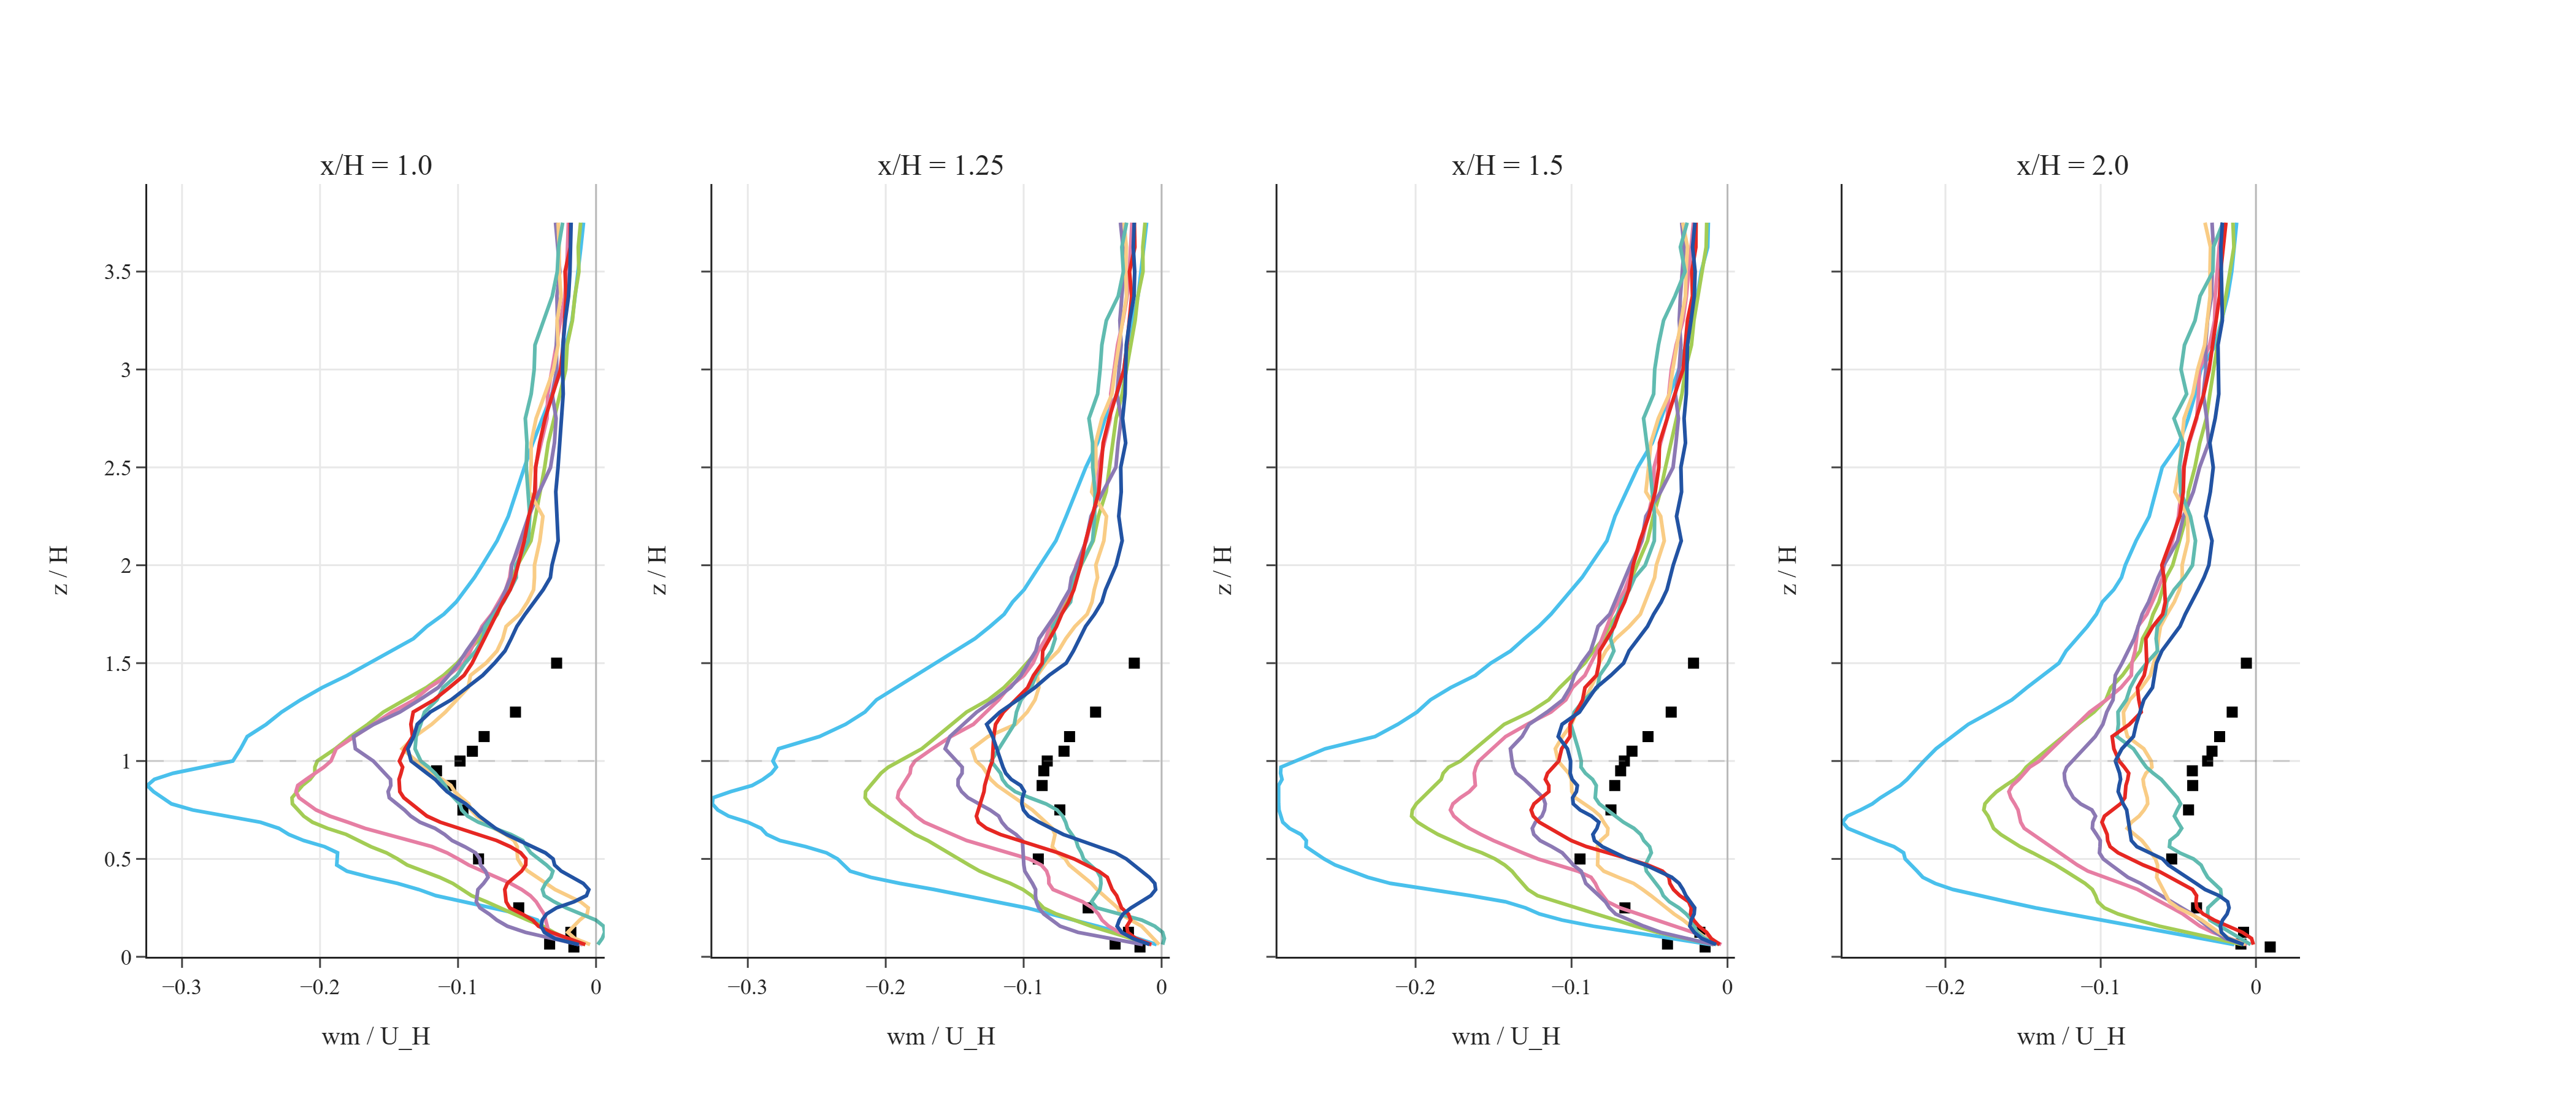
\includegraphics[width=0.85\textwidth]{figures/multi_case_comparisons_z0change/multi_case_comparison_wm_part3.png}
        \caption{}
    \end{subfigure}
    \caption{Normalized mean spanwise velocity ($\bar{w}/U_H$) profiles at (a) $x/H = -1.0$ to $-0.25$, (b) $x/H = 0.0$ to $0.75$, and (c) $x/H = 1.0$ to $2.0$.}
    \label{fig:results_wm}
\end{figure}

\autoref{fig:results_wm} illustrates the vertical profiles of the normalized vertical wind speed ($w/U_H$). These results provide the most significant insights into the model's performance, as they reveal a clear sensitivity to the approach flow conditions. At the initial inflow location ($x/H = -1.0$), there is a general underprediction of the vertical velocity. However, as the flow reaches $x/H = -0.75$, the profiles across all cases show relatively good agreement with the experimental data. A critical discrepancy emerges at the building's center-line ($x/H = -0.25$), where the case lacking approach roughness significantly overpredicts the upward vertical velocity. This overprediction becomes more pronounced in the leeward wake regions (behind the building), where the negative vertical wind speed—representing the downwash in the recirculation zone—is overestimated by a significant margin. This bias persists in the lower-roughness cases, albeit to a lesser degree, but is relatively well-mitigated in Cases 5 through 8. Notably, these successful cases either employ larger roughness blocks (24 m and 32 m in Cases 5 and 6) or combine moderate blocks (16 m and 20 m) with an increased surface roughness parameter ($z_0 = 0.1$ in Cases 7 and 8). This suggests that a specific threshold of turbulent intensity and surface friction is required to correctly model the vertical momentum exchange in the building's near-field.

% --- Streamwise Fluctuations (u_rms) ---
\begin{figure}[htbp]
    \centering
    \begin{subfigure}[b]{\textwidth}
        \centering
        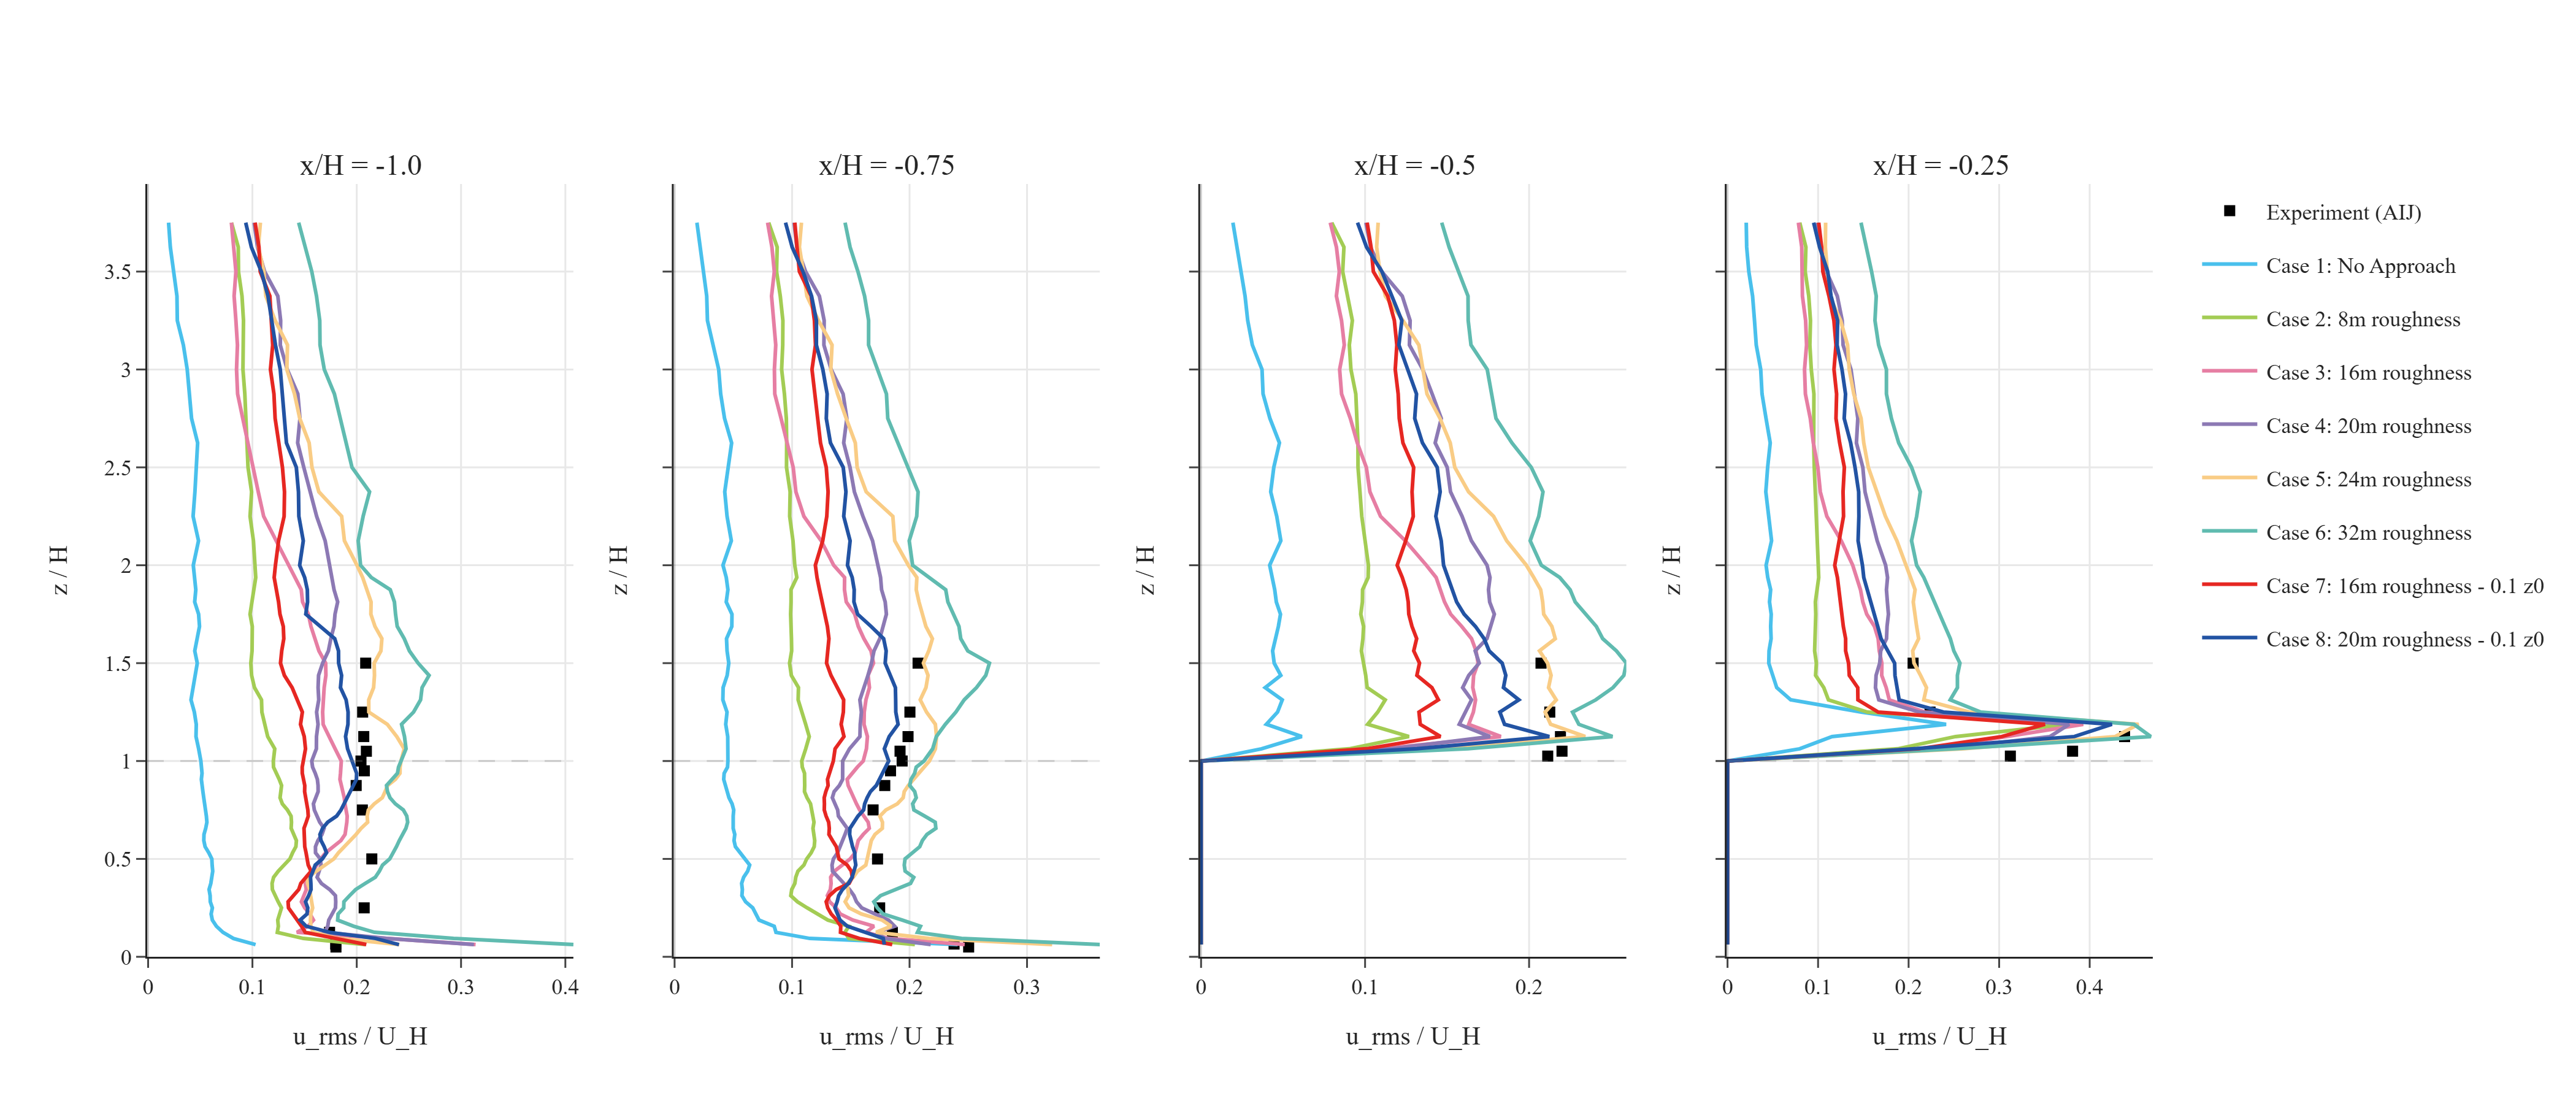
\includegraphics[width=0.85\textwidth]{figures/multi_case_comparisons_z0change/u/comparison_u_rms_part1.png}
        \caption{}
    \end{subfigure}
    \vspace{1ex}
    \begin{subfigure}[b]{\textwidth}
        \centering
        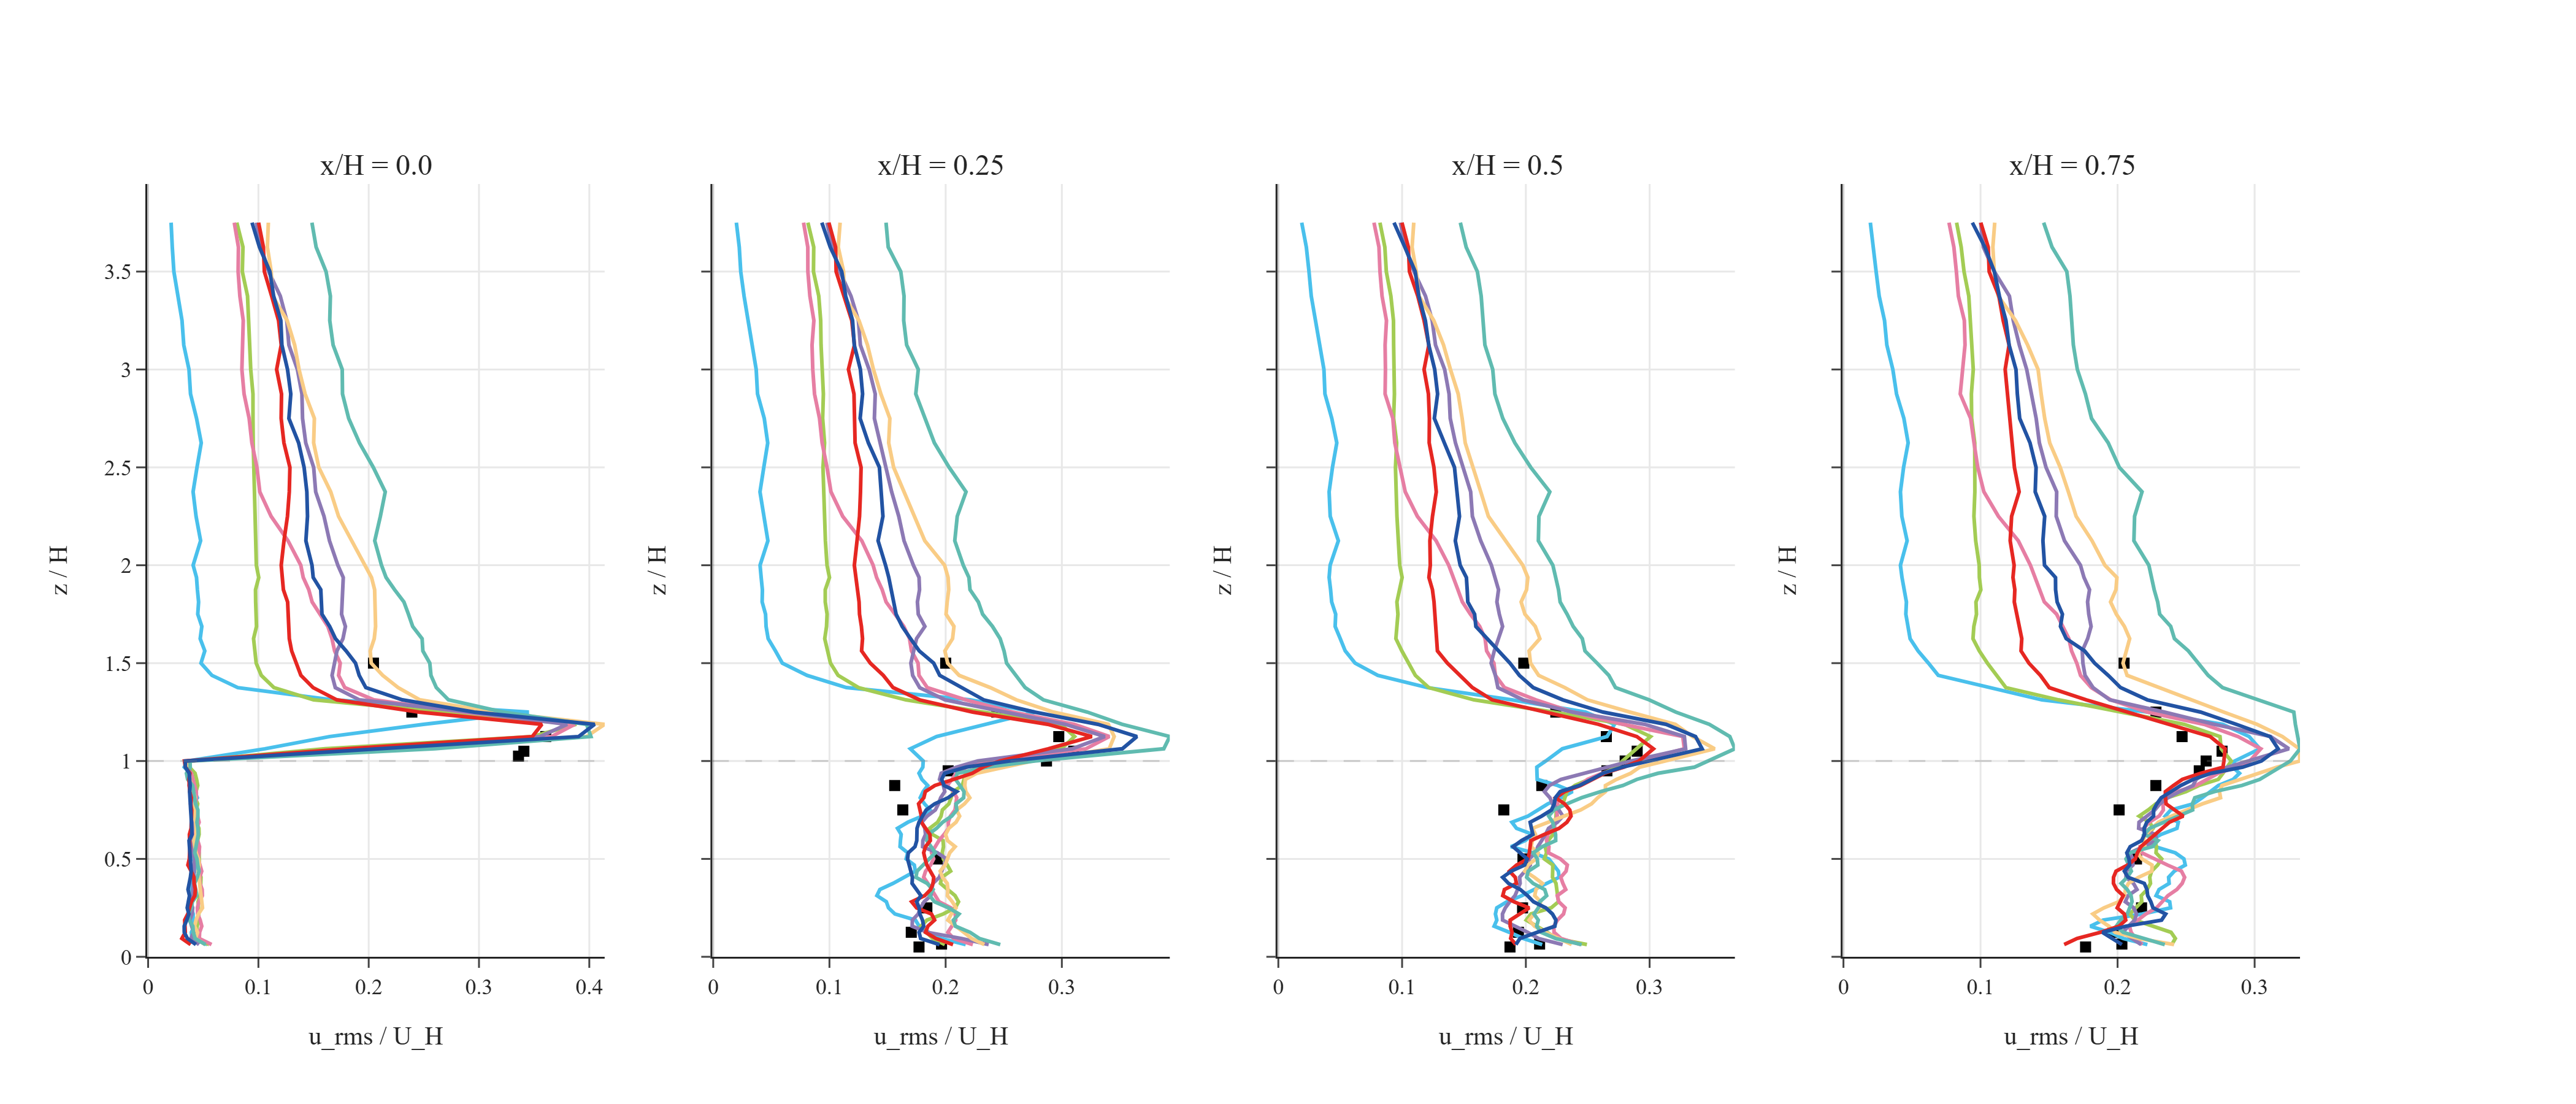
\includegraphics[width=0.85\textwidth]{figures/multi_case_comparisons_z0change/u/comparison_u_rms_part2.png}
        \caption{}
    \end{subfigure}
    \vspace{1ex}
    \begin{subfigure}[b]{\textwidth}
        \centering
        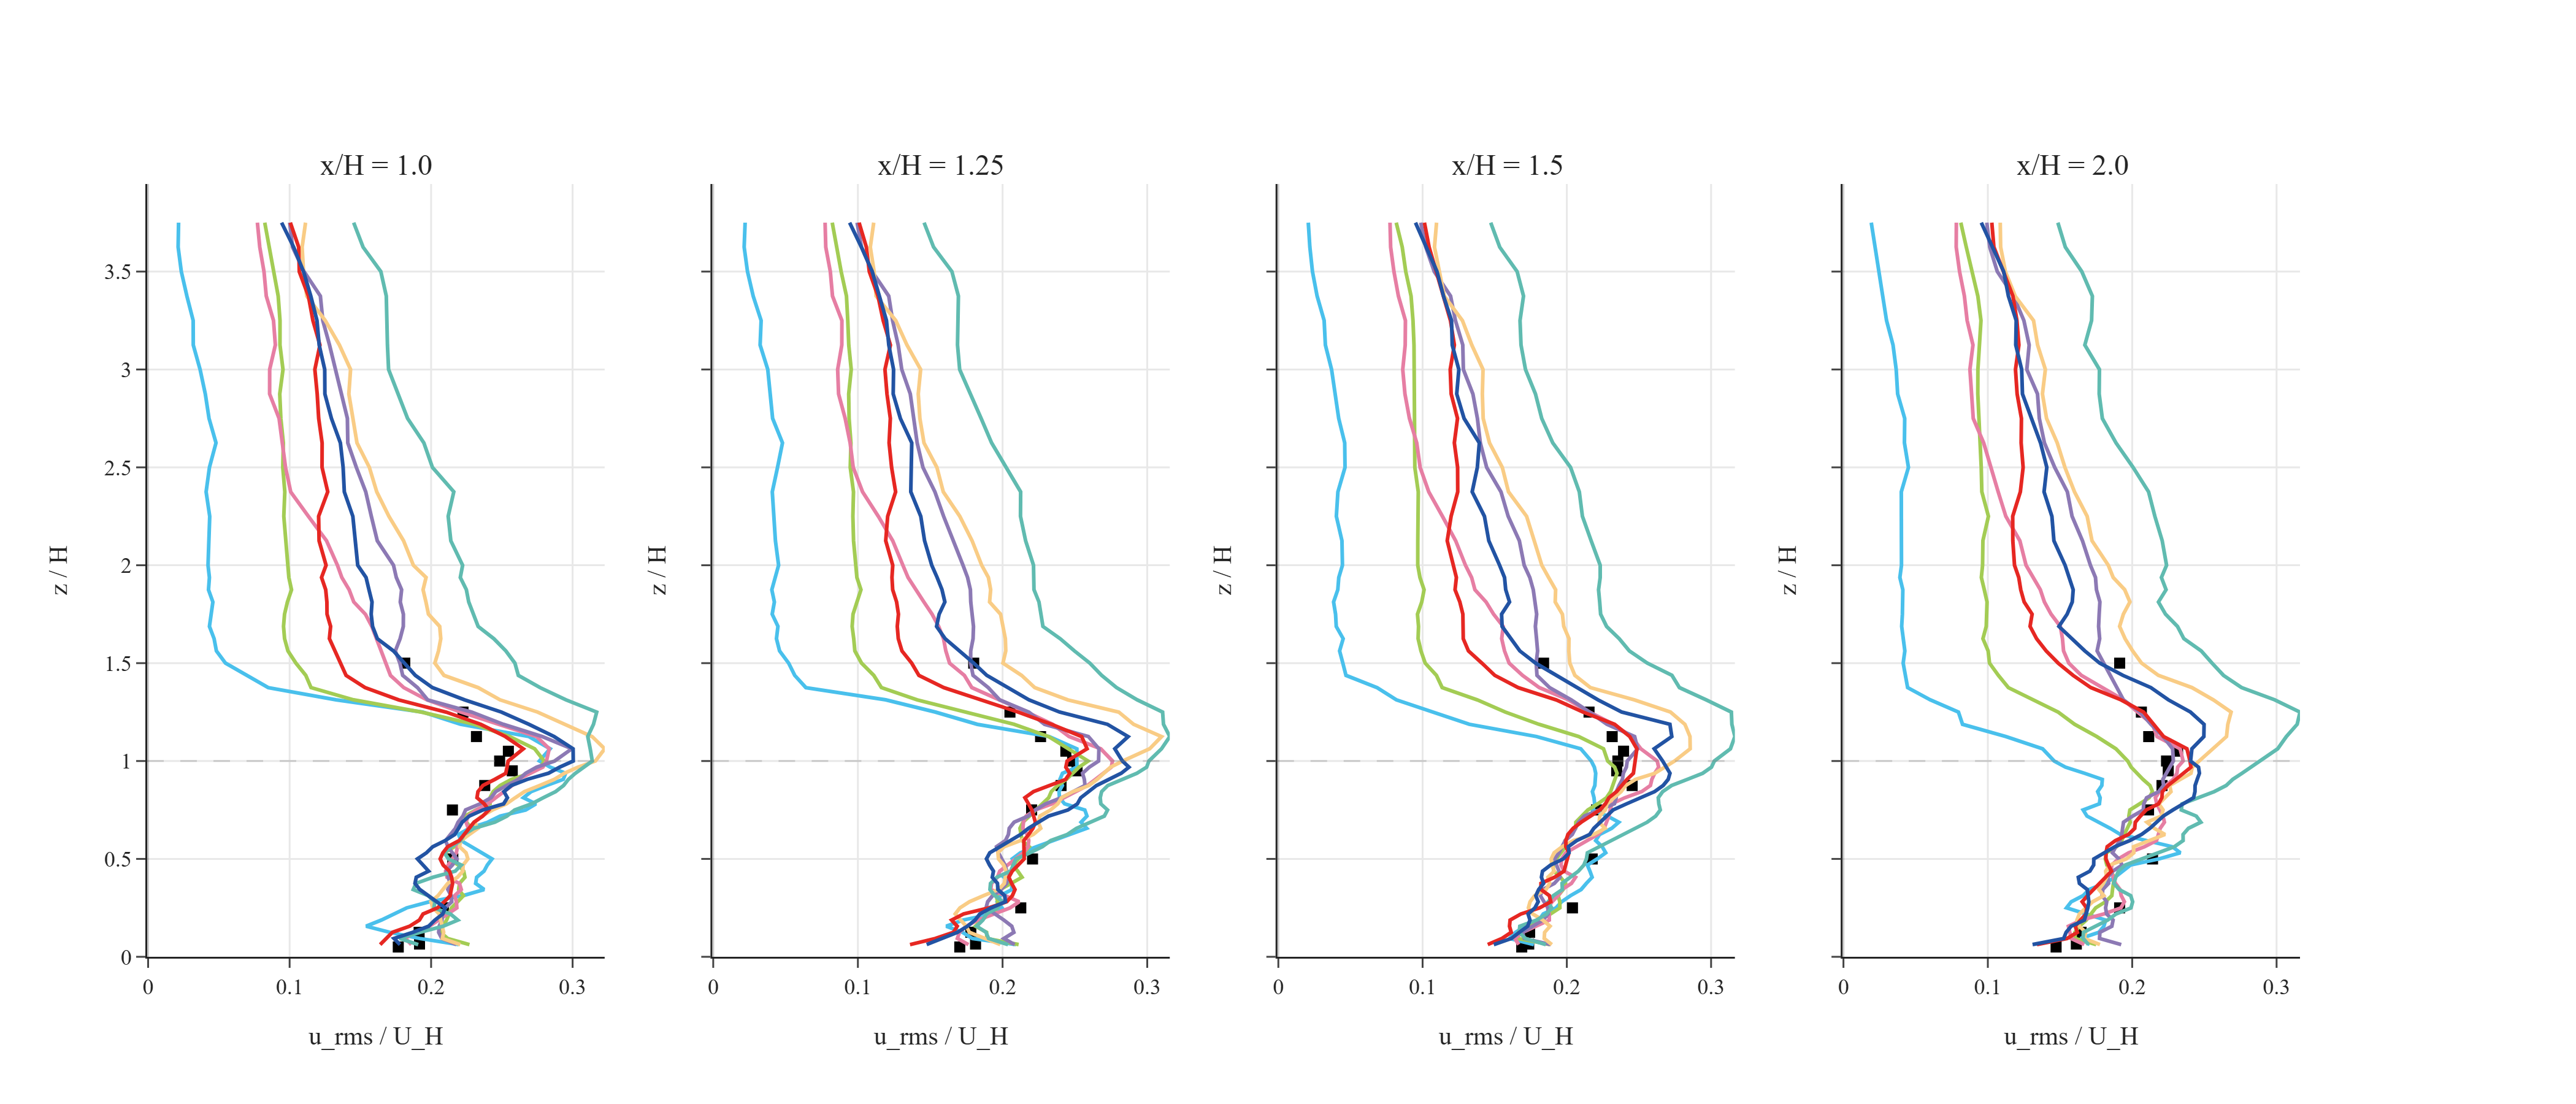
\includegraphics[width=0.85\textwidth]{figures/multi_case_comparisons_z0change/u/comparison_u_rms_part3.png}
        \caption{}
    \end{subfigure}
    \caption{Normalized streamwise velocity fluctuations ($u_{rms}/U_H$) at (a) Upwind/Rooftop, (b) Leeward Side ($x/H=0$ to $0.75$), and (c) Downwind Wake ($x/H=1.0$ to $2.0$).}
    \label{fig:results_urms}
\end{figure}

\autoref{fig:results_urms} illustrates the vertical profiles of the root-mean-square (RMS) streamwise velocity fluctuations ($u_{rms}/U_H$). Unlike the mean velocity profiles, which showed general agreement across most cases, the $u_{rms}$ results exhibit significant variability depending on the approach roughness. In the windward approach region ($x/H = -1.0$), the velocity variation is notably underpredicted, particularly in the case lacking an approach section. Accuracy improves as the roughness block size increases; however, the largest blocks (Cases 5 and 6) lead to a slight overprediction of the turbulence intensity. Directly above the building, the high-roughness cases and the medium-roughness cases with increased $z_0$ provide the most accurate predictions, while the case with no roughness severely underpredicts the fluctuations. In the immediate leeward wake, all cases capture the general pattern of the profile. Small roughness cases tend toward slight underprediction, whereas larger roughness blocks result in a slight overprediction. The discrepancy becomes most prominent in the far-wake region. Here, the no-roughness case fails to maintain the turbulent energy, leading to a severe underprediction of the profile. Conversely, while higher roughness slightly overestimates the variation, Cases 3 and 4 (medium roughness) and Cases 7 and 8 (medium roughness with increased $z_0$) demonstrate the highest overall predictive accuracy. This suggests that moderate turbulence levels best replicate the balanced energy state observed in the wind tunnel experiments.

% --- Spanwise Fluctuations (v_rms) ---
\begin{figure}[htbp]
    \centering
    \begin{subfigure}[b]{\textwidth}
        \centering
        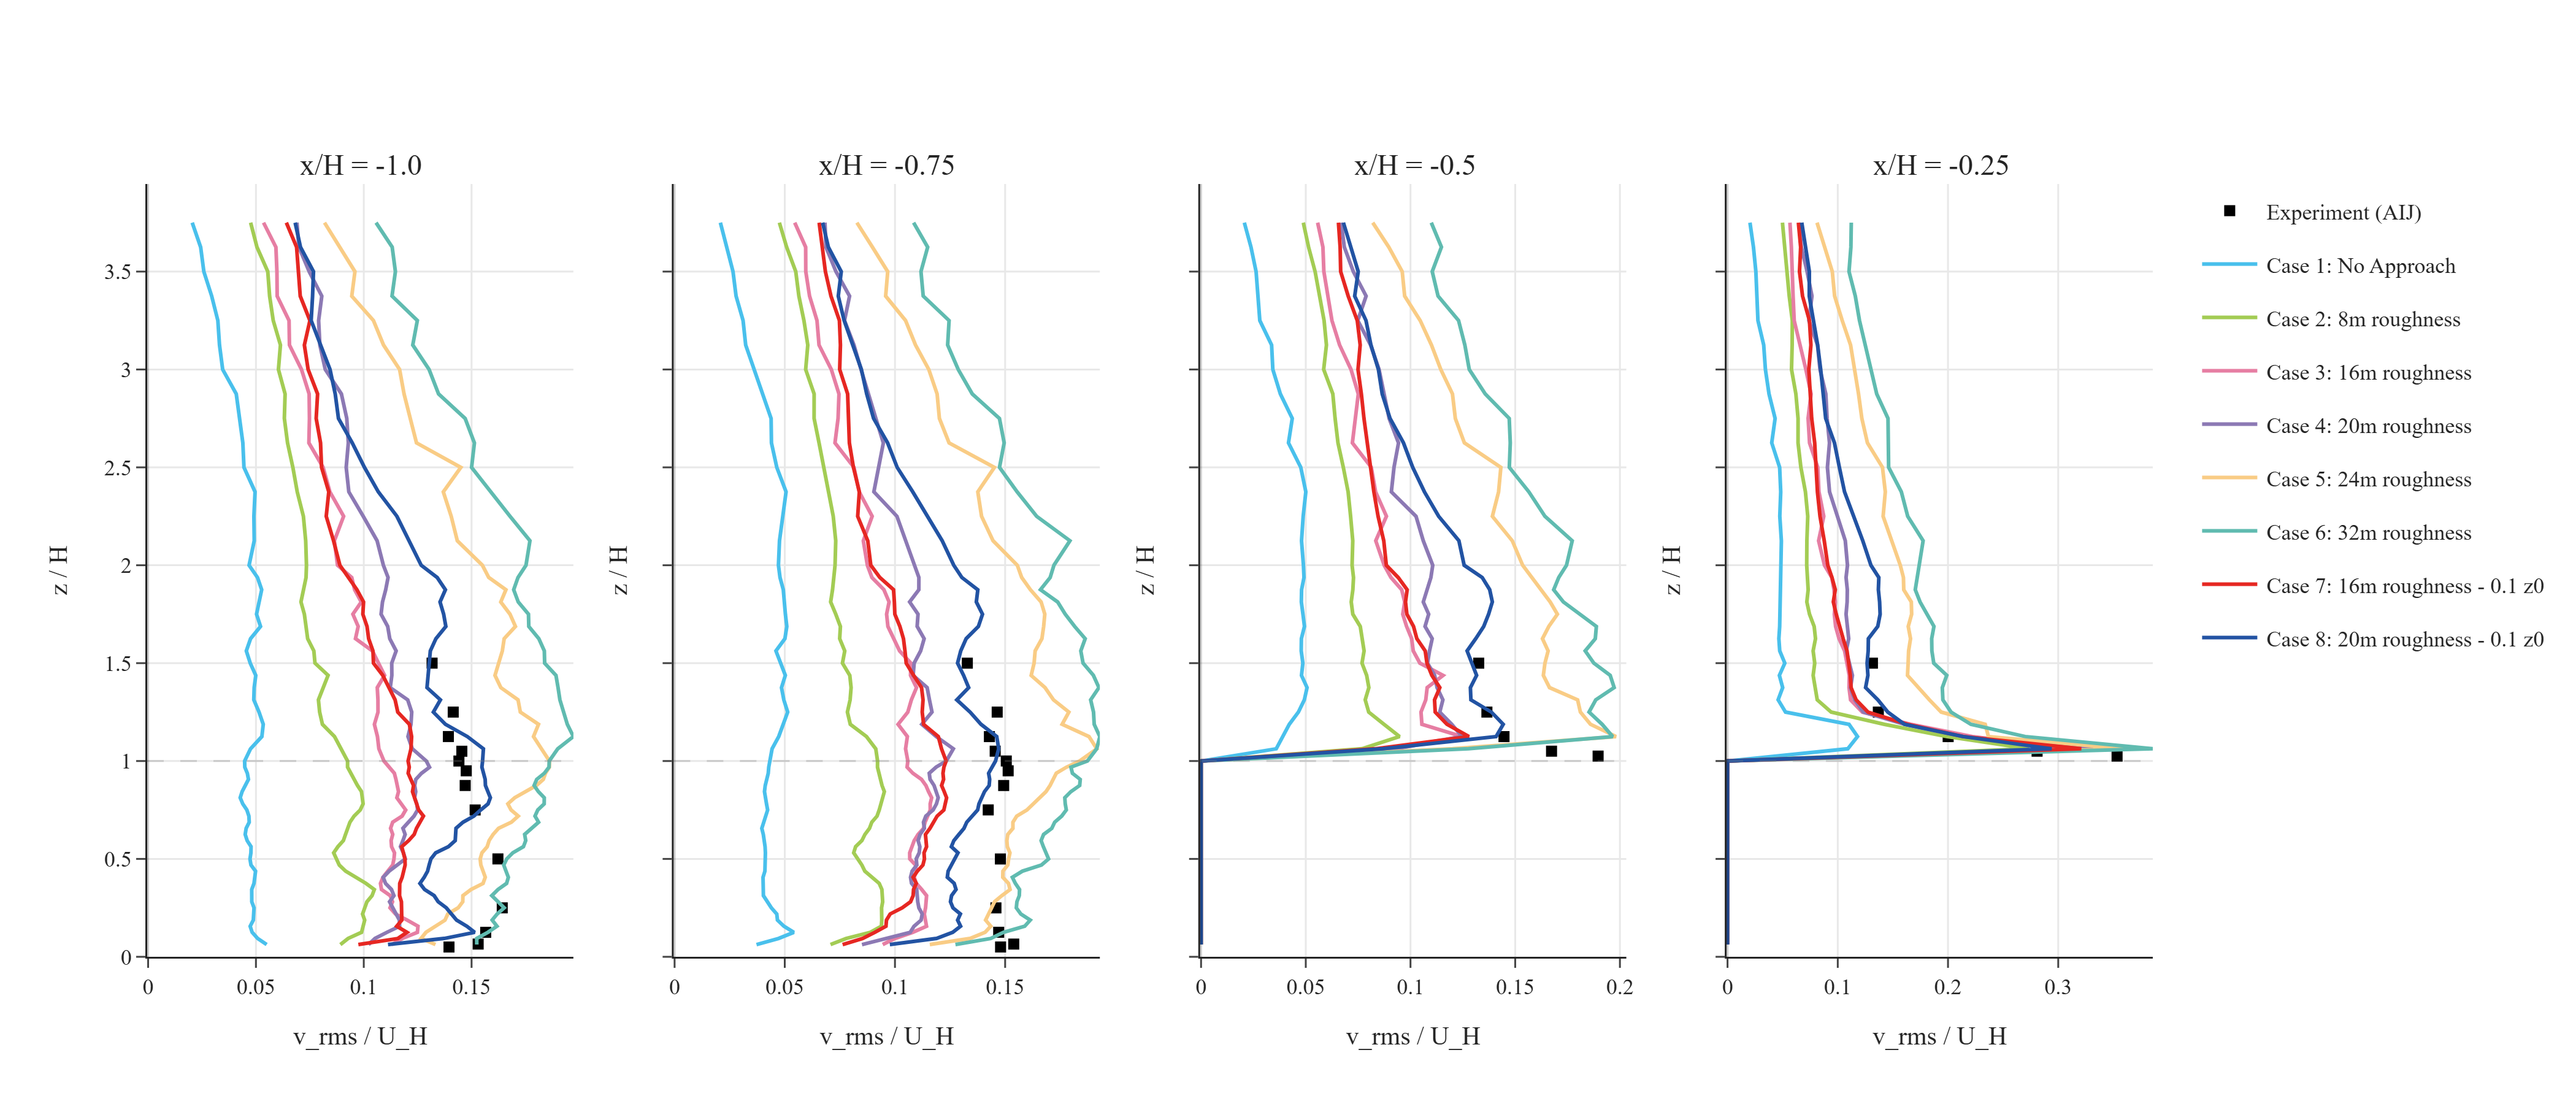
\includegraphics[width=0.85\textwidth]{figures/multi_case_comparisons_z0change/v/comparison_v_rms_part1.png}
        \caption{}
    \end{subfigure}
    \vspace{1ex}
    \begin{subfigure}[b]{\textwidth}
        \centering
        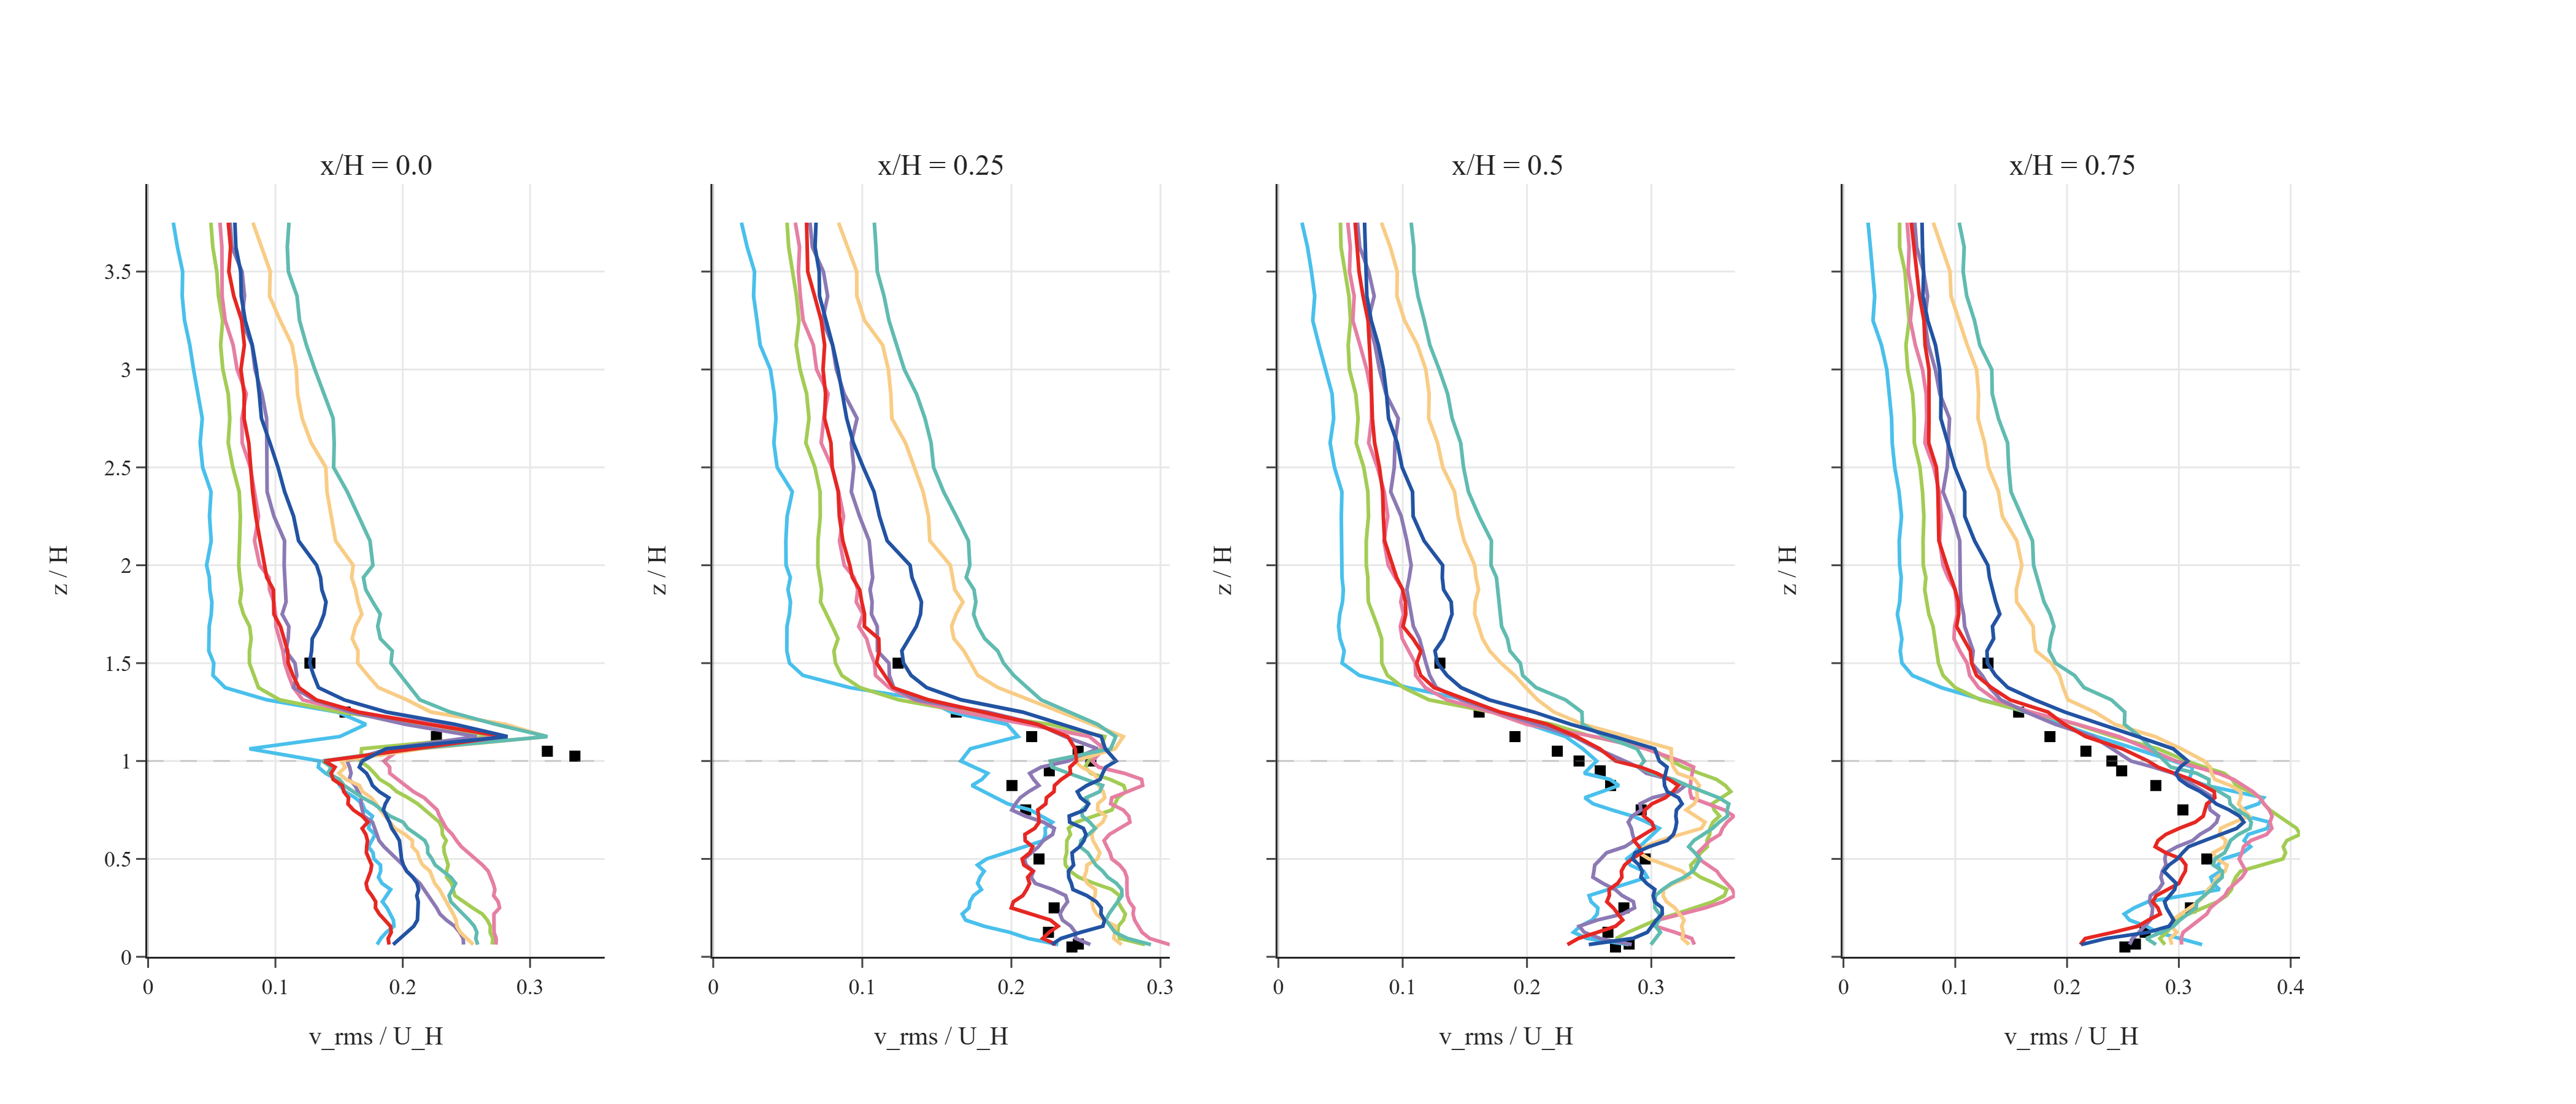
\includegraphics[width=0.85\textwidth]{figures/multi_case_comparisons_z0change/v/comparison_v_rms_part2.png}
        \caption{}
    \end{subfigure}
    \vspace{1ex}
    \begin{subfigure}[b]{\textwidth}
        \centering
        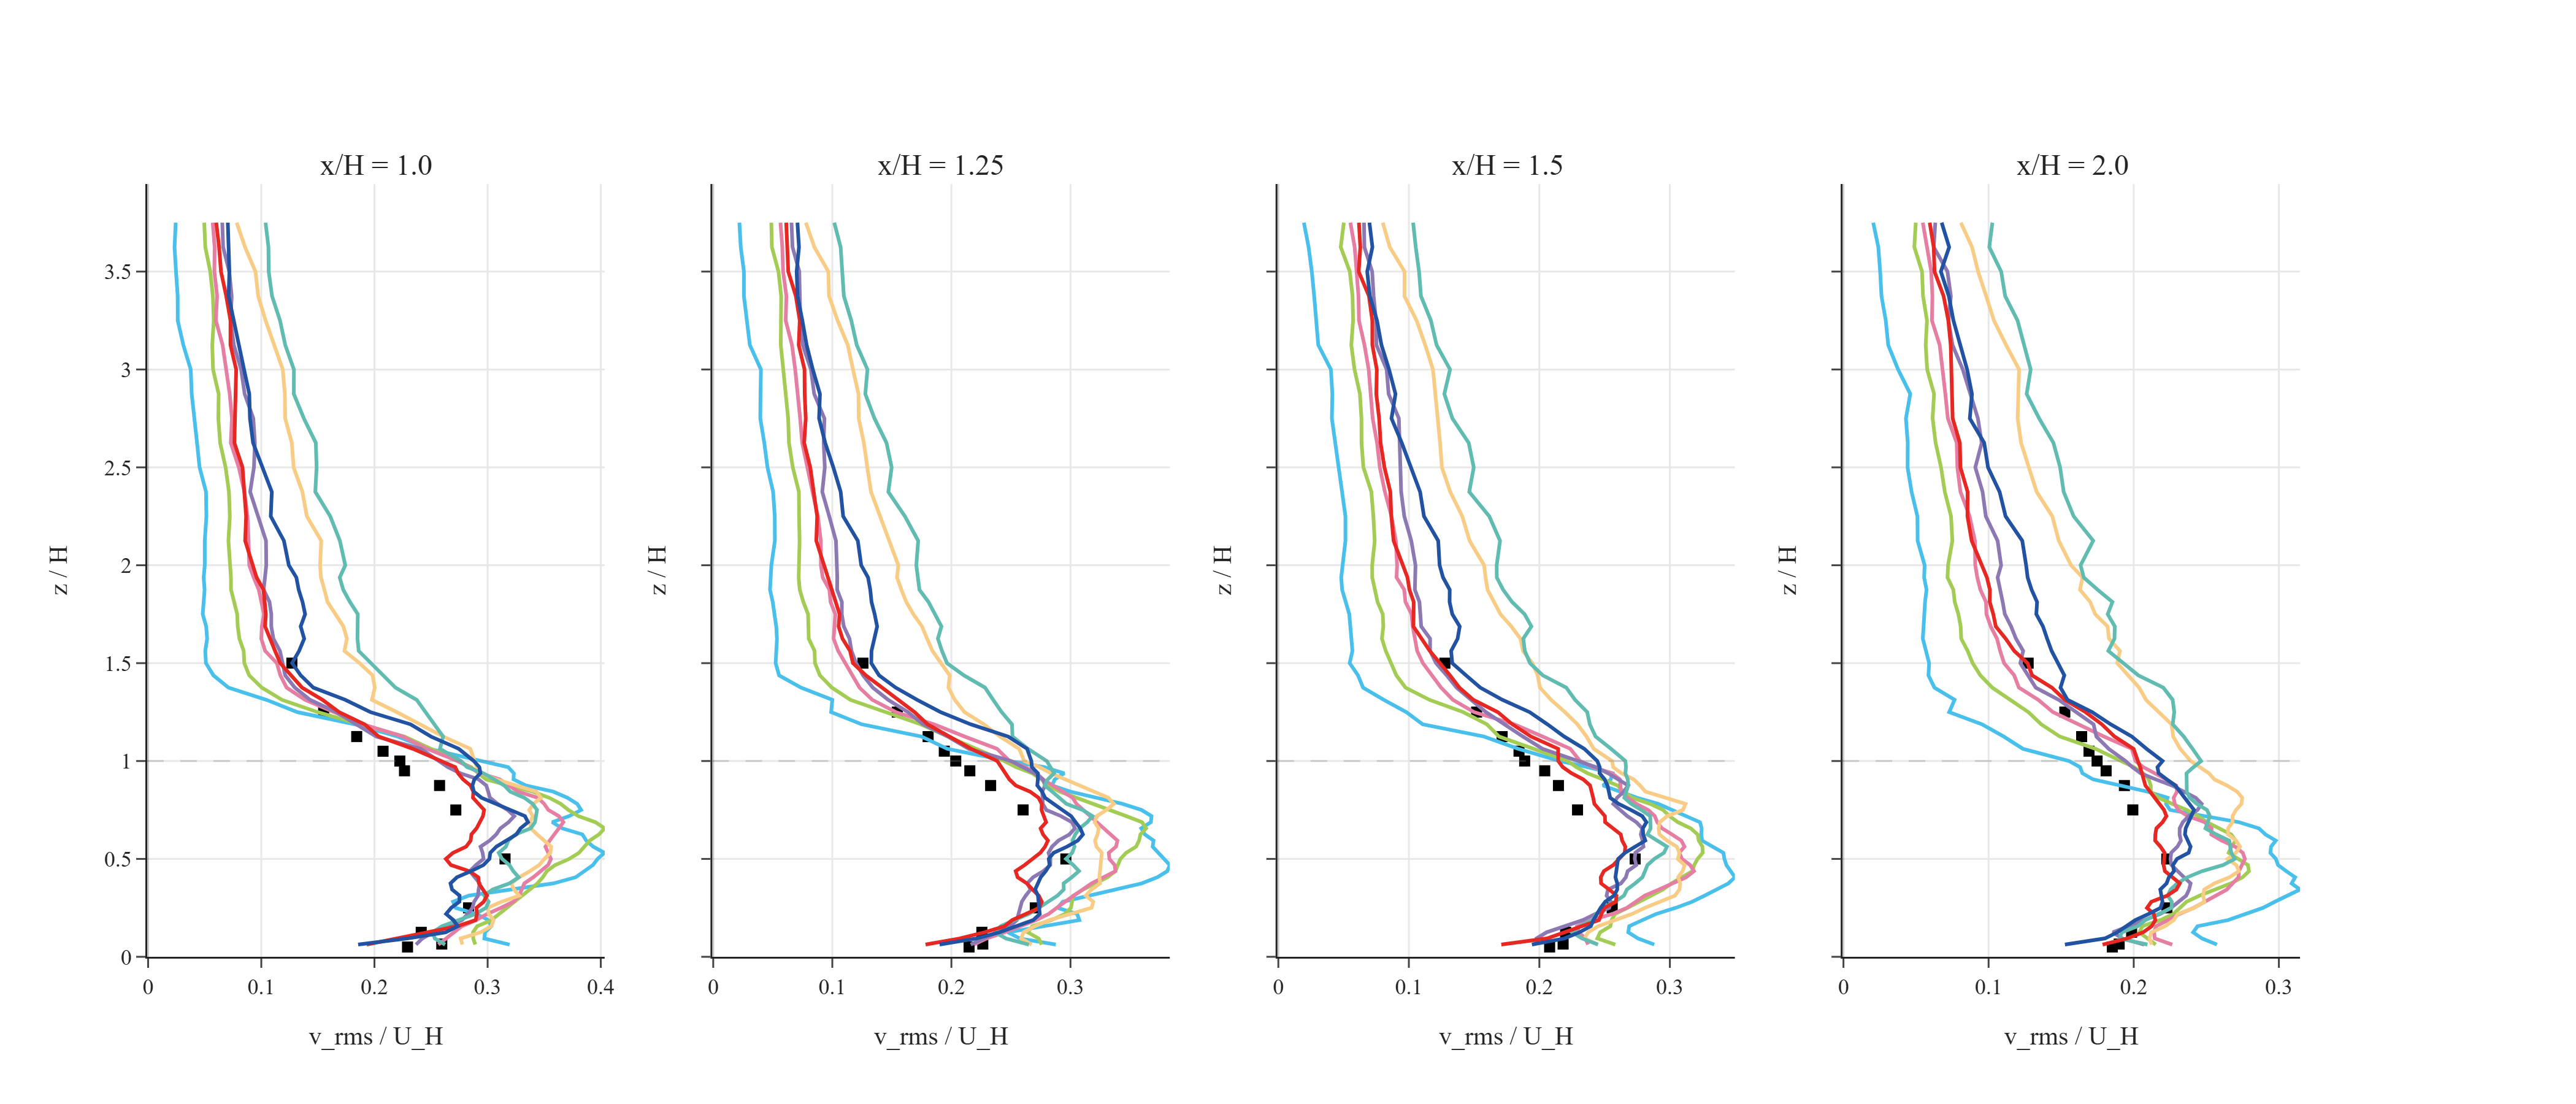
\includegraphics[width=0.85\textwidth]{figures/multi_case_comparisons_z0change/v/comparison_v_rms_part3.png}
        \caption{}
    \end{subfigure}
    \caption{Normalized spanwise velocity fluctuations ($v_{rms}/U_H$) at (a) Upwind/Rooftop, (b) Leeward Side ($x/H=0$ to $0.75$), and (c) Downwind Wake ($x/H=1.0$ to $2.0$).}
    \label{fig:results_vrms}
\end{figure}

\autoref{fig:results_vrms} presents the vertical profiles of the normalized spanwise velocity fluctuations ($v_{rms}/U_H$). Similar to the observations in the $u_{rms}$ results, the approach section without roughness severely underpredicts the spanwise turbulence levels. Conversely, the cases with the largest roughness blocks (Cases 5 and 6) lead to an overprediction of these fluctuations in the windward region. Interestingly, while the high-roughness cases provide the most accurate predictions directly above the building, this accuracy transitions into a magnitude overprediction as the flow enters the leeward wake. A notable phenomenon occurs in the no-roughness case behind the building: rather than a simple underprediction, the model produces a significant overprediction of $v_{rms}$ with a distinct change in the profile shape. In these instances, the variation is characterized by a sharp peak reaching at height 0.5 $H$, whereas the experimental data and the more accurate simulation cases show a smoother, more stable curvature. While the large roughness blocks also overpredict the magnitude in the wake, they maintain the correct physical shape of the profile. Consistent with the results of other velocity components, the medium-roughness cases (Cases 3 and 4) and those combining medium roughness with increased surface friction (Cases 7 and 8) demonstrate the most reliable results overall. These cases avoid both the numerical instability seen in the no-roughness peaks and the excessive energy associated with the largest roughness obstacles.

% --- Vertical Fluctuations (w_rms) ---
\begin{figure}[htbp]
    \centering
    \begin{subfigure}[b]{\textwidth}
        \centering
        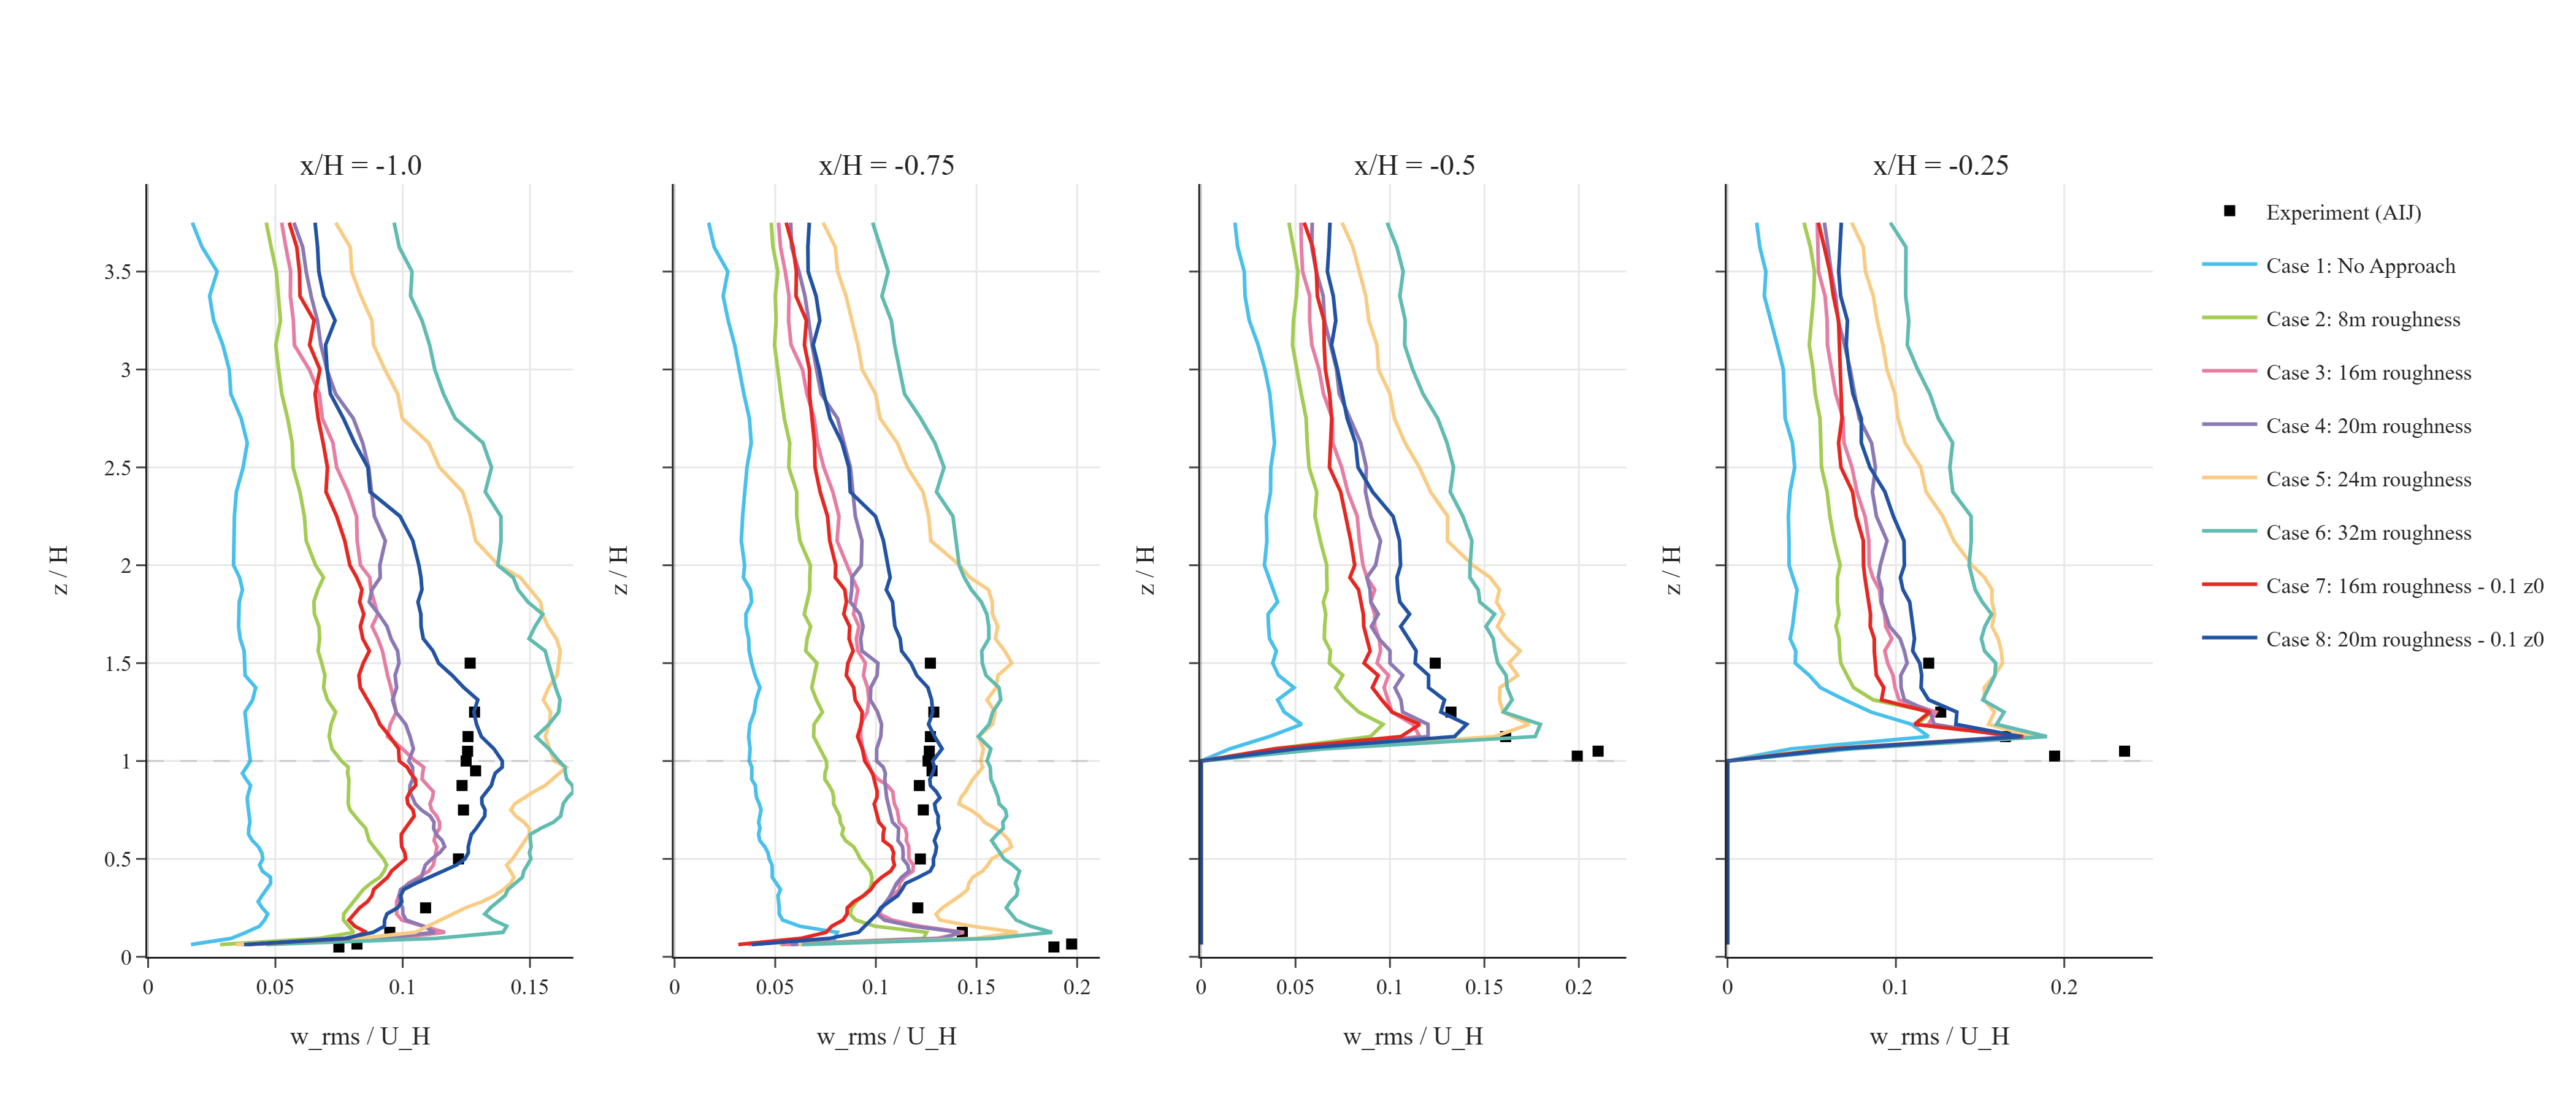
\includegraphics[width=0.85\textwidth]{figures/multi_case_comparisons_z0change/w/comparison_w_rms_part1.png}
        \caption{}
    \end{subfigure}
    \vspace{1ex}
    \begin{subfigure}[b]{\textwidth}
        \centering
        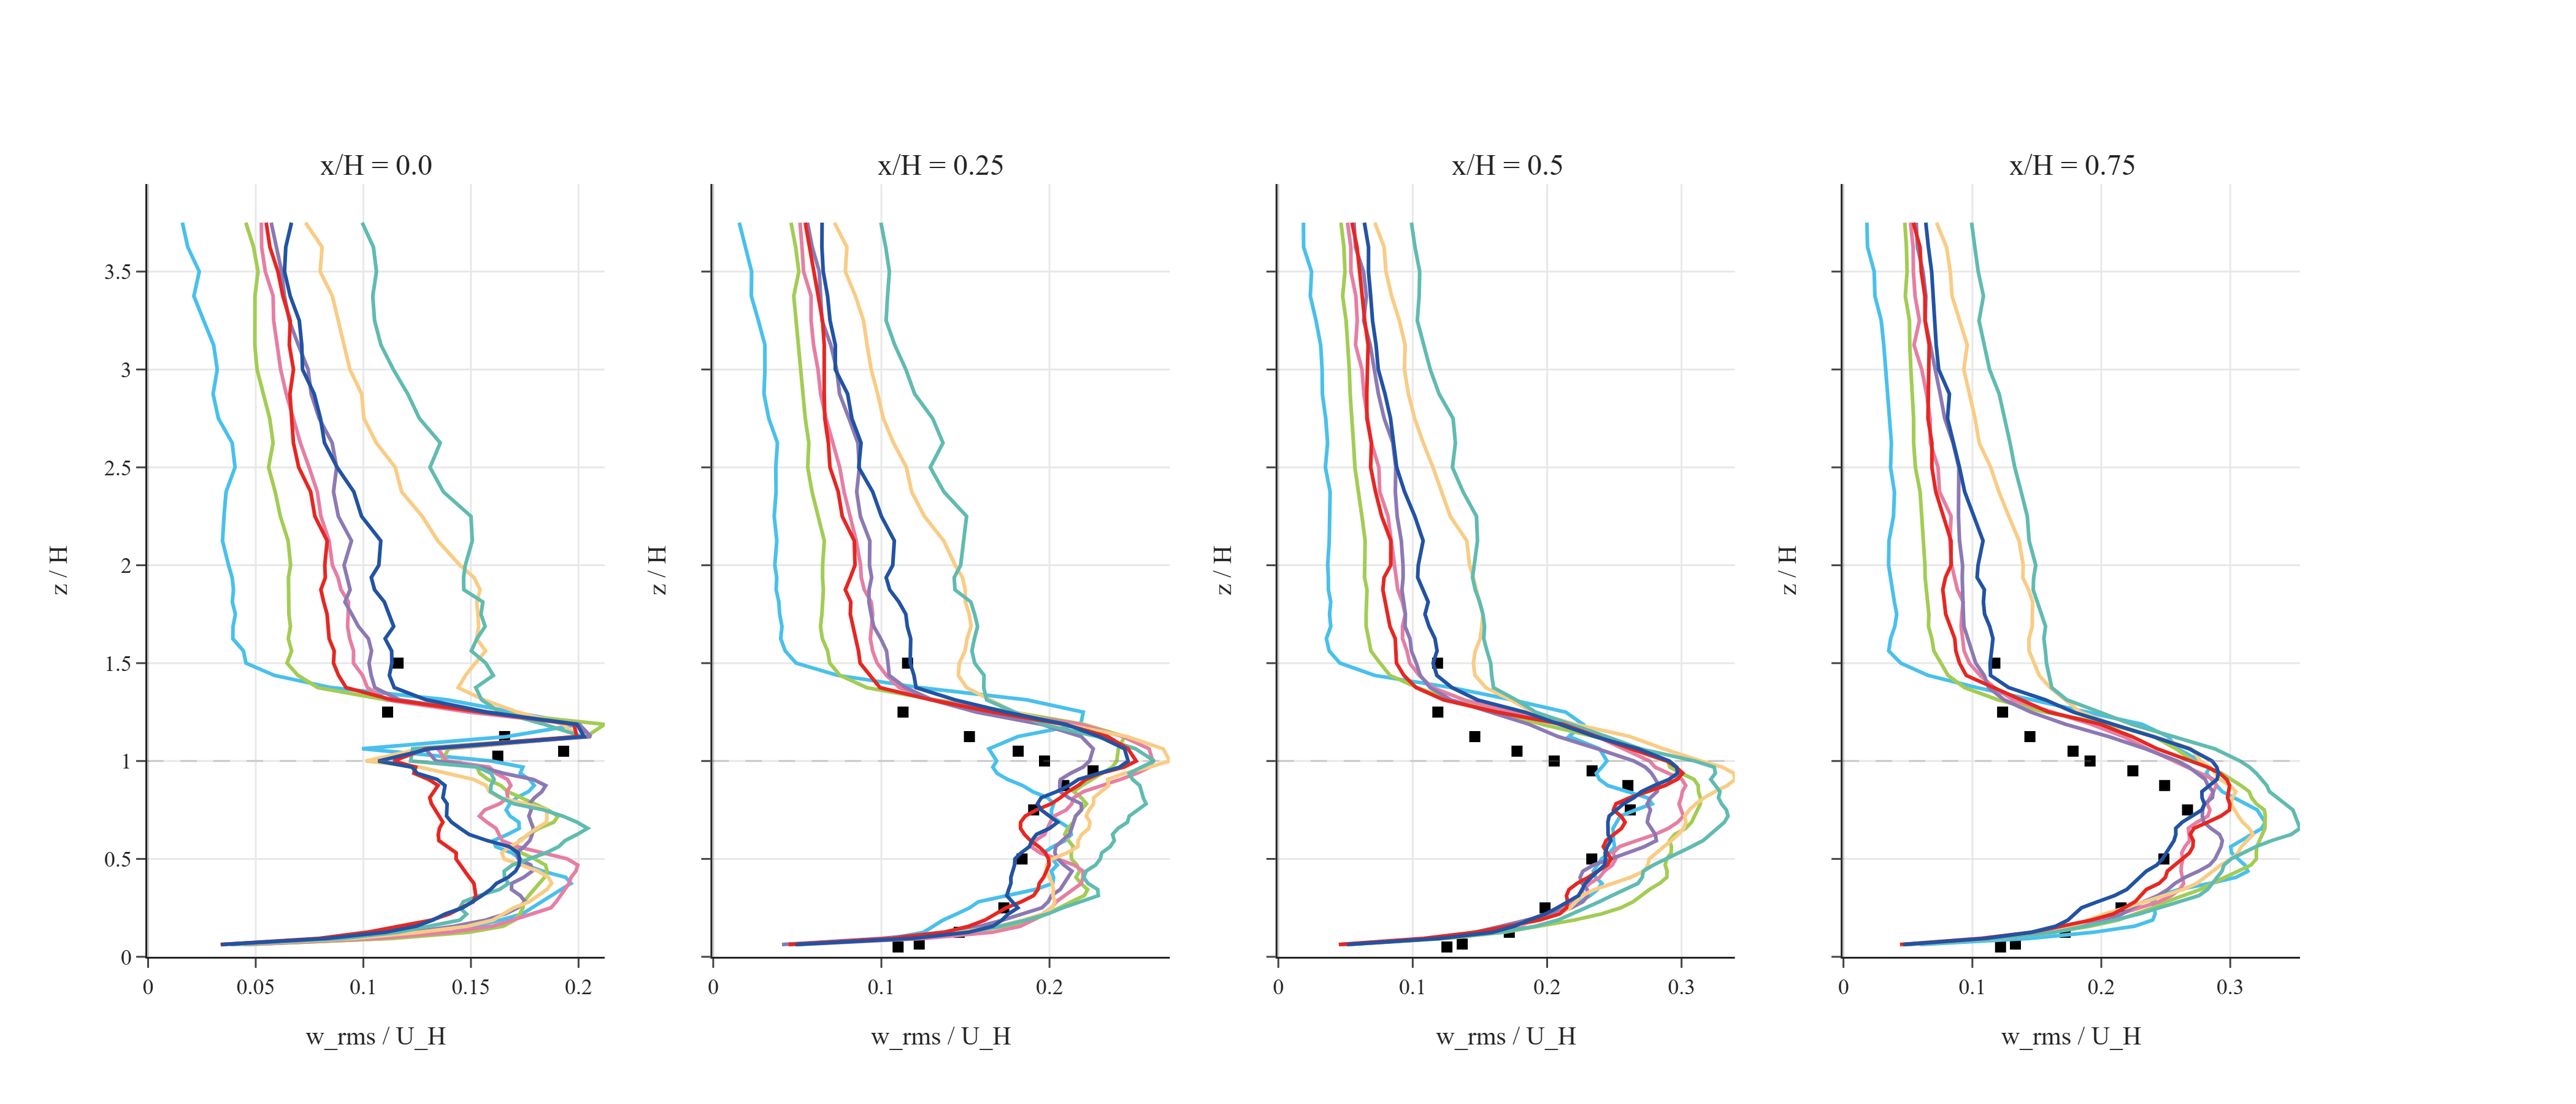
\includegraphics[width=0.85\textwidth]{figures/multi_case_comparisons_z0change/w/comparison_w_rms_part2.png}
        \caption{}
    \end{subfigure}
    \vspace{1ex}
    \begin{subfigure}[b]{\textwidth}
        \centering
        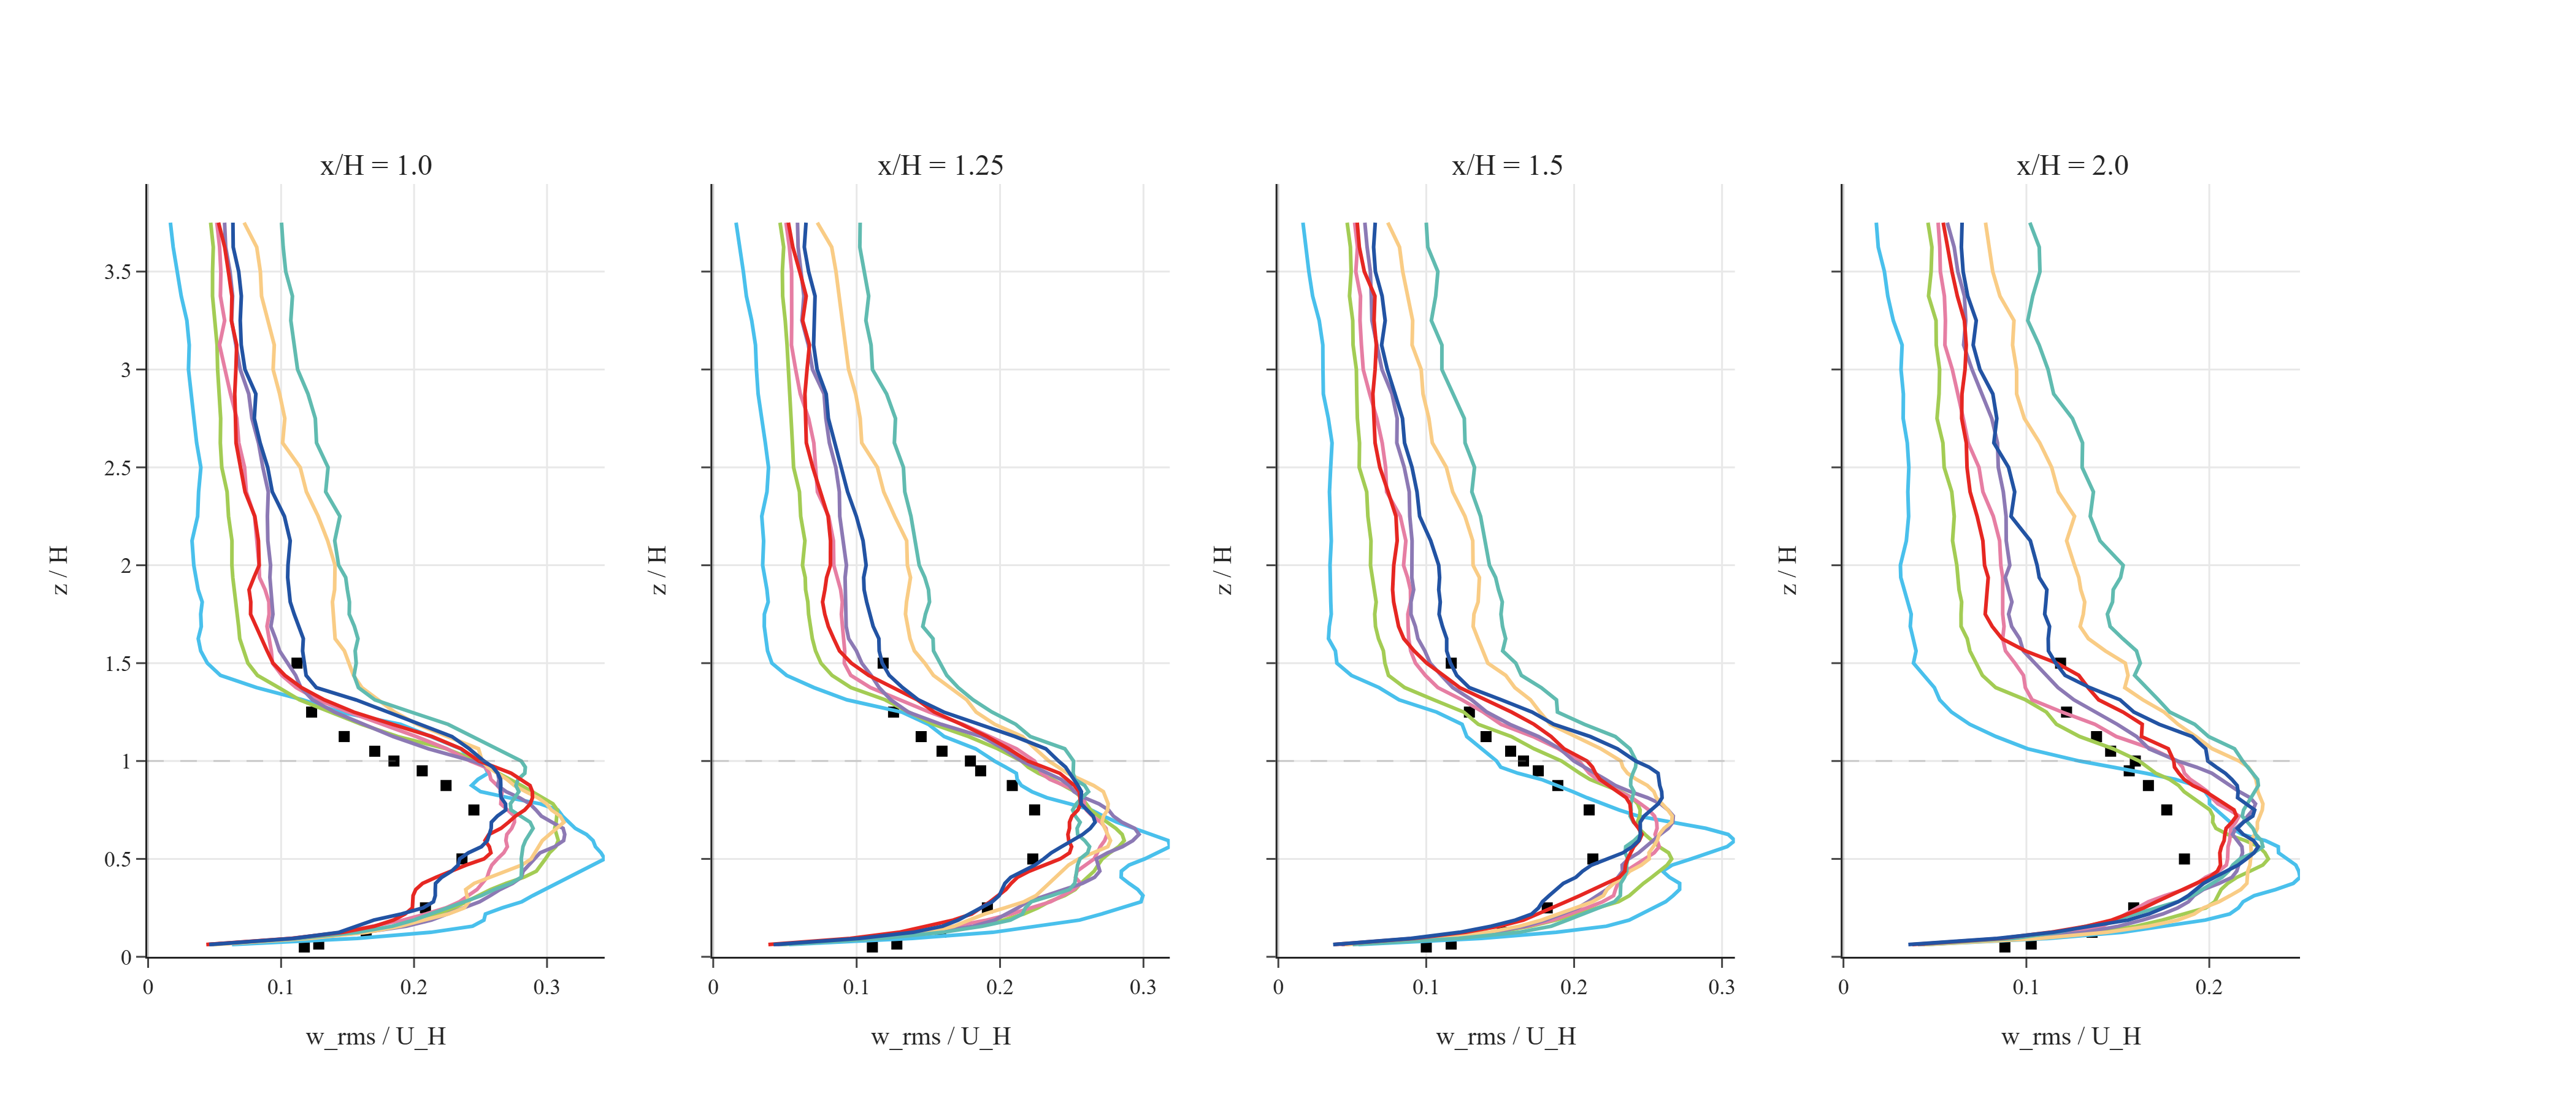
\includegraphics[width=0.85\textwidth]{figures/multi_case_comparisons_z0change/w/comparison_w_rms_part3.png}
        \caption{}
    \end{subfigure}
    \caption{Normalized vertical velocity fluctuations ($w_{rms}/U_H$) at (a) Upwind/Rooftop, (b) Leeward Side ($x/H=0$ to $0.75$), and (c) Downwind Wake ($x/H=1.0$ to $2.0$).}
    \label{fig:results_wrms}
\end{figure}

\autoref{fig:results_wrms} illustrates the vertical profiles of the normalized vertical velocity fluctuations ($w_{rms}/U_H$). The results closely mirror the patterns observed in the spanwise fluctuations ($v_{rms}$), both in terms of magnitude and profile shape. A recurring phenomenon is observed in the case without an approach section, which exhibits a sharp, non-physical peak in the leeward wake. This sharp peak matches the position and anomalous shape seen in the $v_{rms}$ results, further suggesting that the absence of upstream turbulence leads to numerical instabilities or an unnatural vortex structure behind the building. For the remaining cases, the patterns of underprediction in low-roughness setups and overprediction in high-roughness setups remain consistent. The profile shapes are nearly identical to those of the $v_{rms}$ cases, with Cases 7 and 8 again providing the most stable and accurate fit to the AIJ wind tunnel data. The similarity between the $v_{rms}$ and $w_{rms}$ profiles indicates that the turbulence in the wake is largely isotropic in its fluctuations, and that the approach flow roughness is the primary factor in correctly capturing this vertical energy distribution.

% --- Turbulent Kinetic Energy (TKE) ---
\begin{figure}[htbp]
    \centering
    \begin{subfigure}[b]{\textwidth}
        \centering
        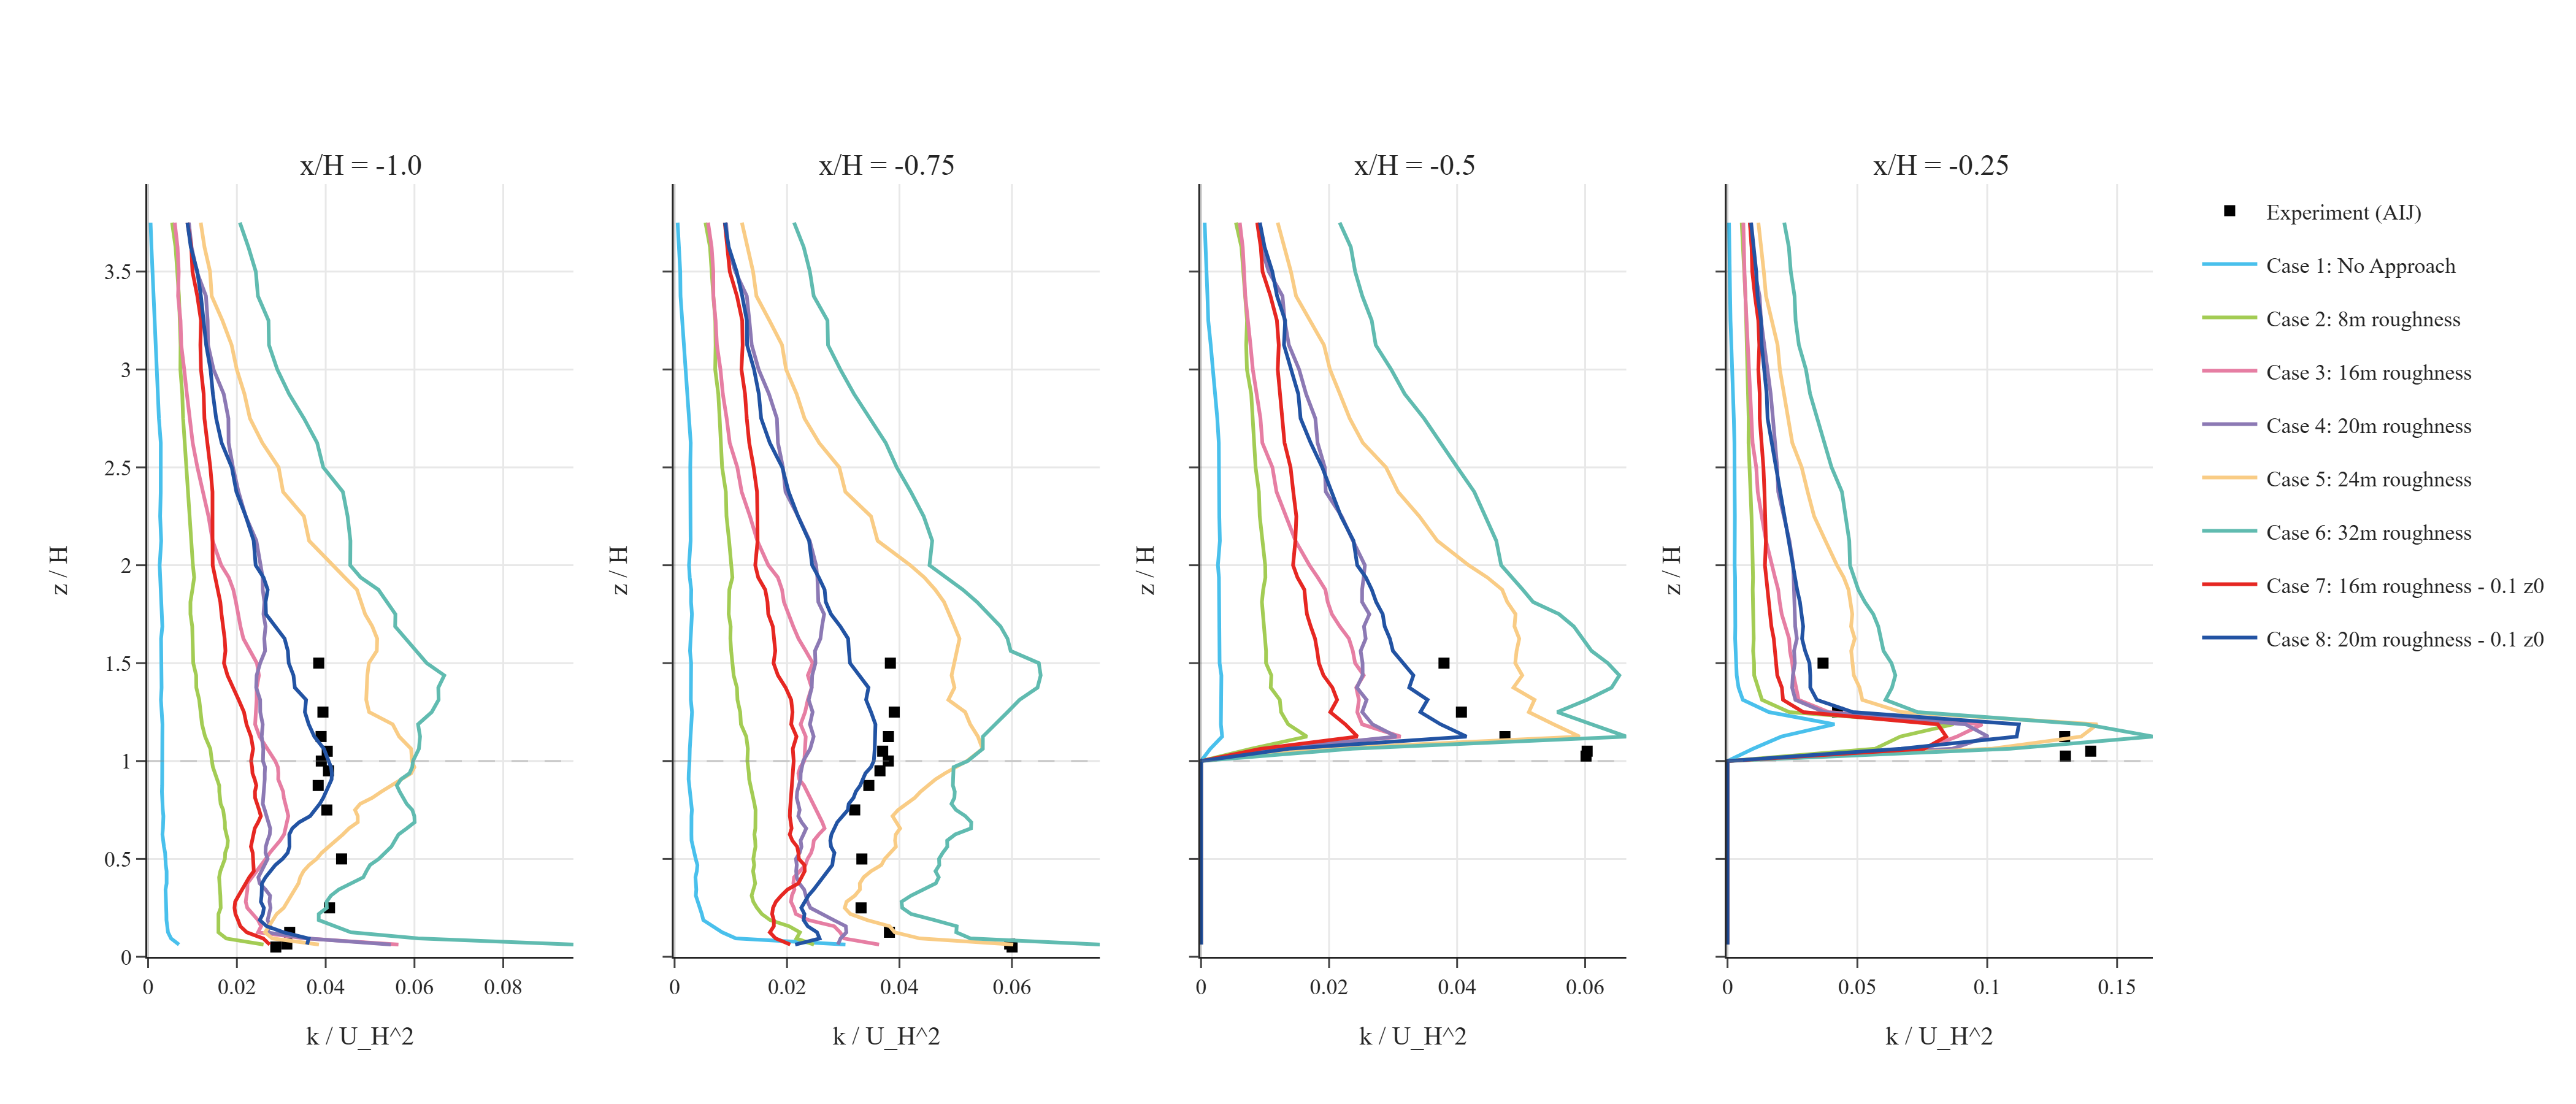
\includegraphics[width=0.85\textwidth]{figures/multi_case_comparisons_z0change/multi_case_comparison_TKE_part1.png}
        \caption{}
    \end{subfigure}
    \vspace{1ex}
    \begin{subfigure}[b]{\textwidth}
        \centering
        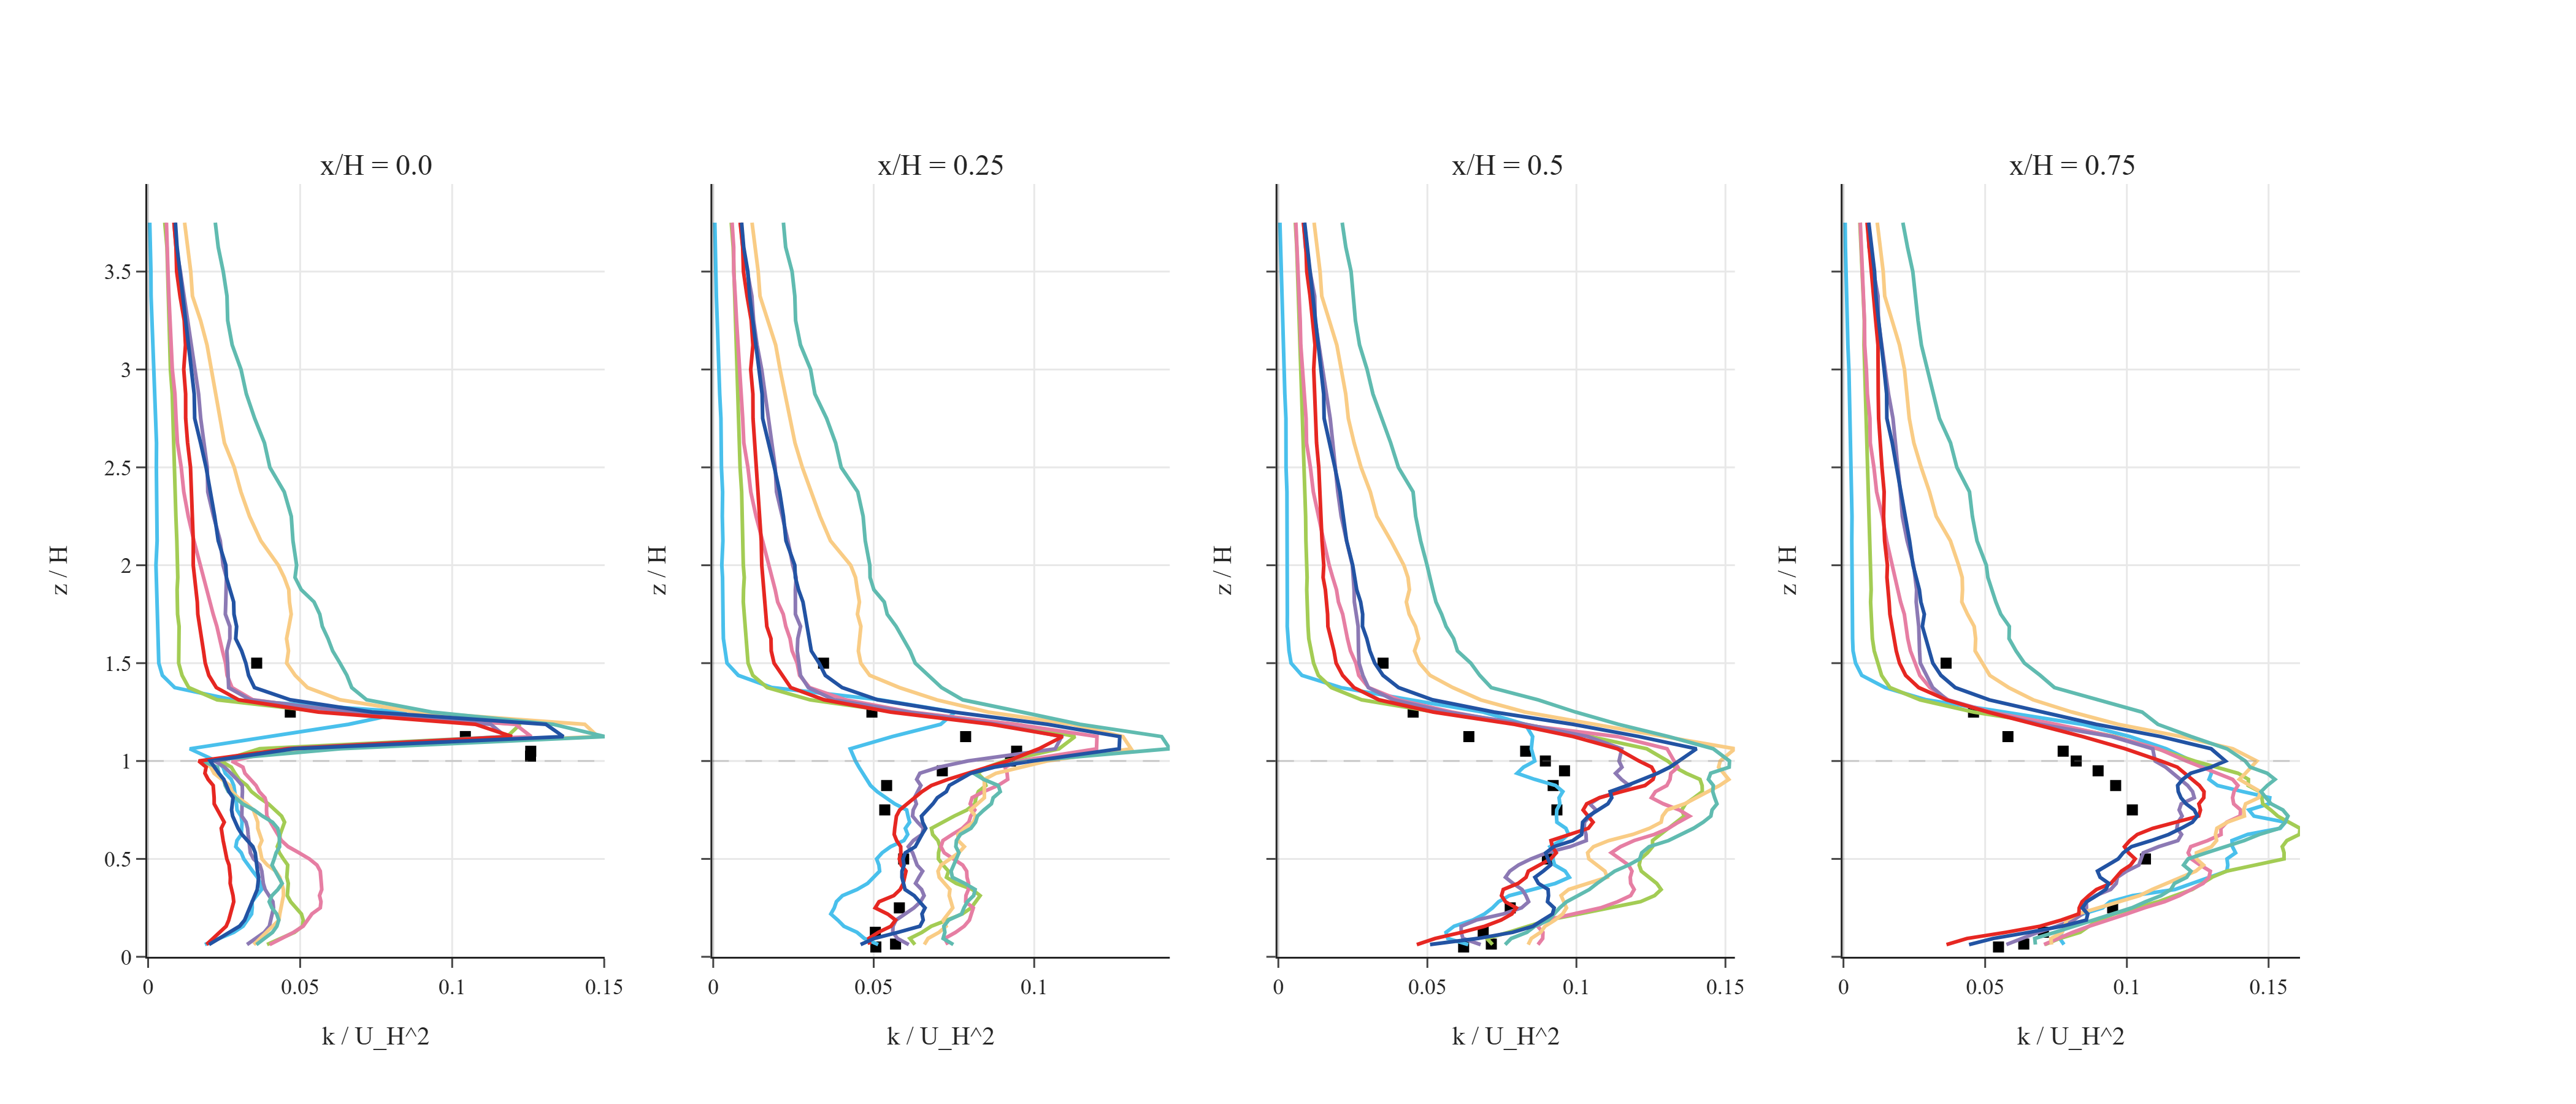
\includegraphics[width=0.85\textwidth]{figures/multi_case_comparisons_z0change/multi_case_comparison_TKE_part2.png}
        \caption{}
    \end{subfigure}
    \vspace{1ex}
    \begin{subfigure}[b]{\textwidth}
        \centering
        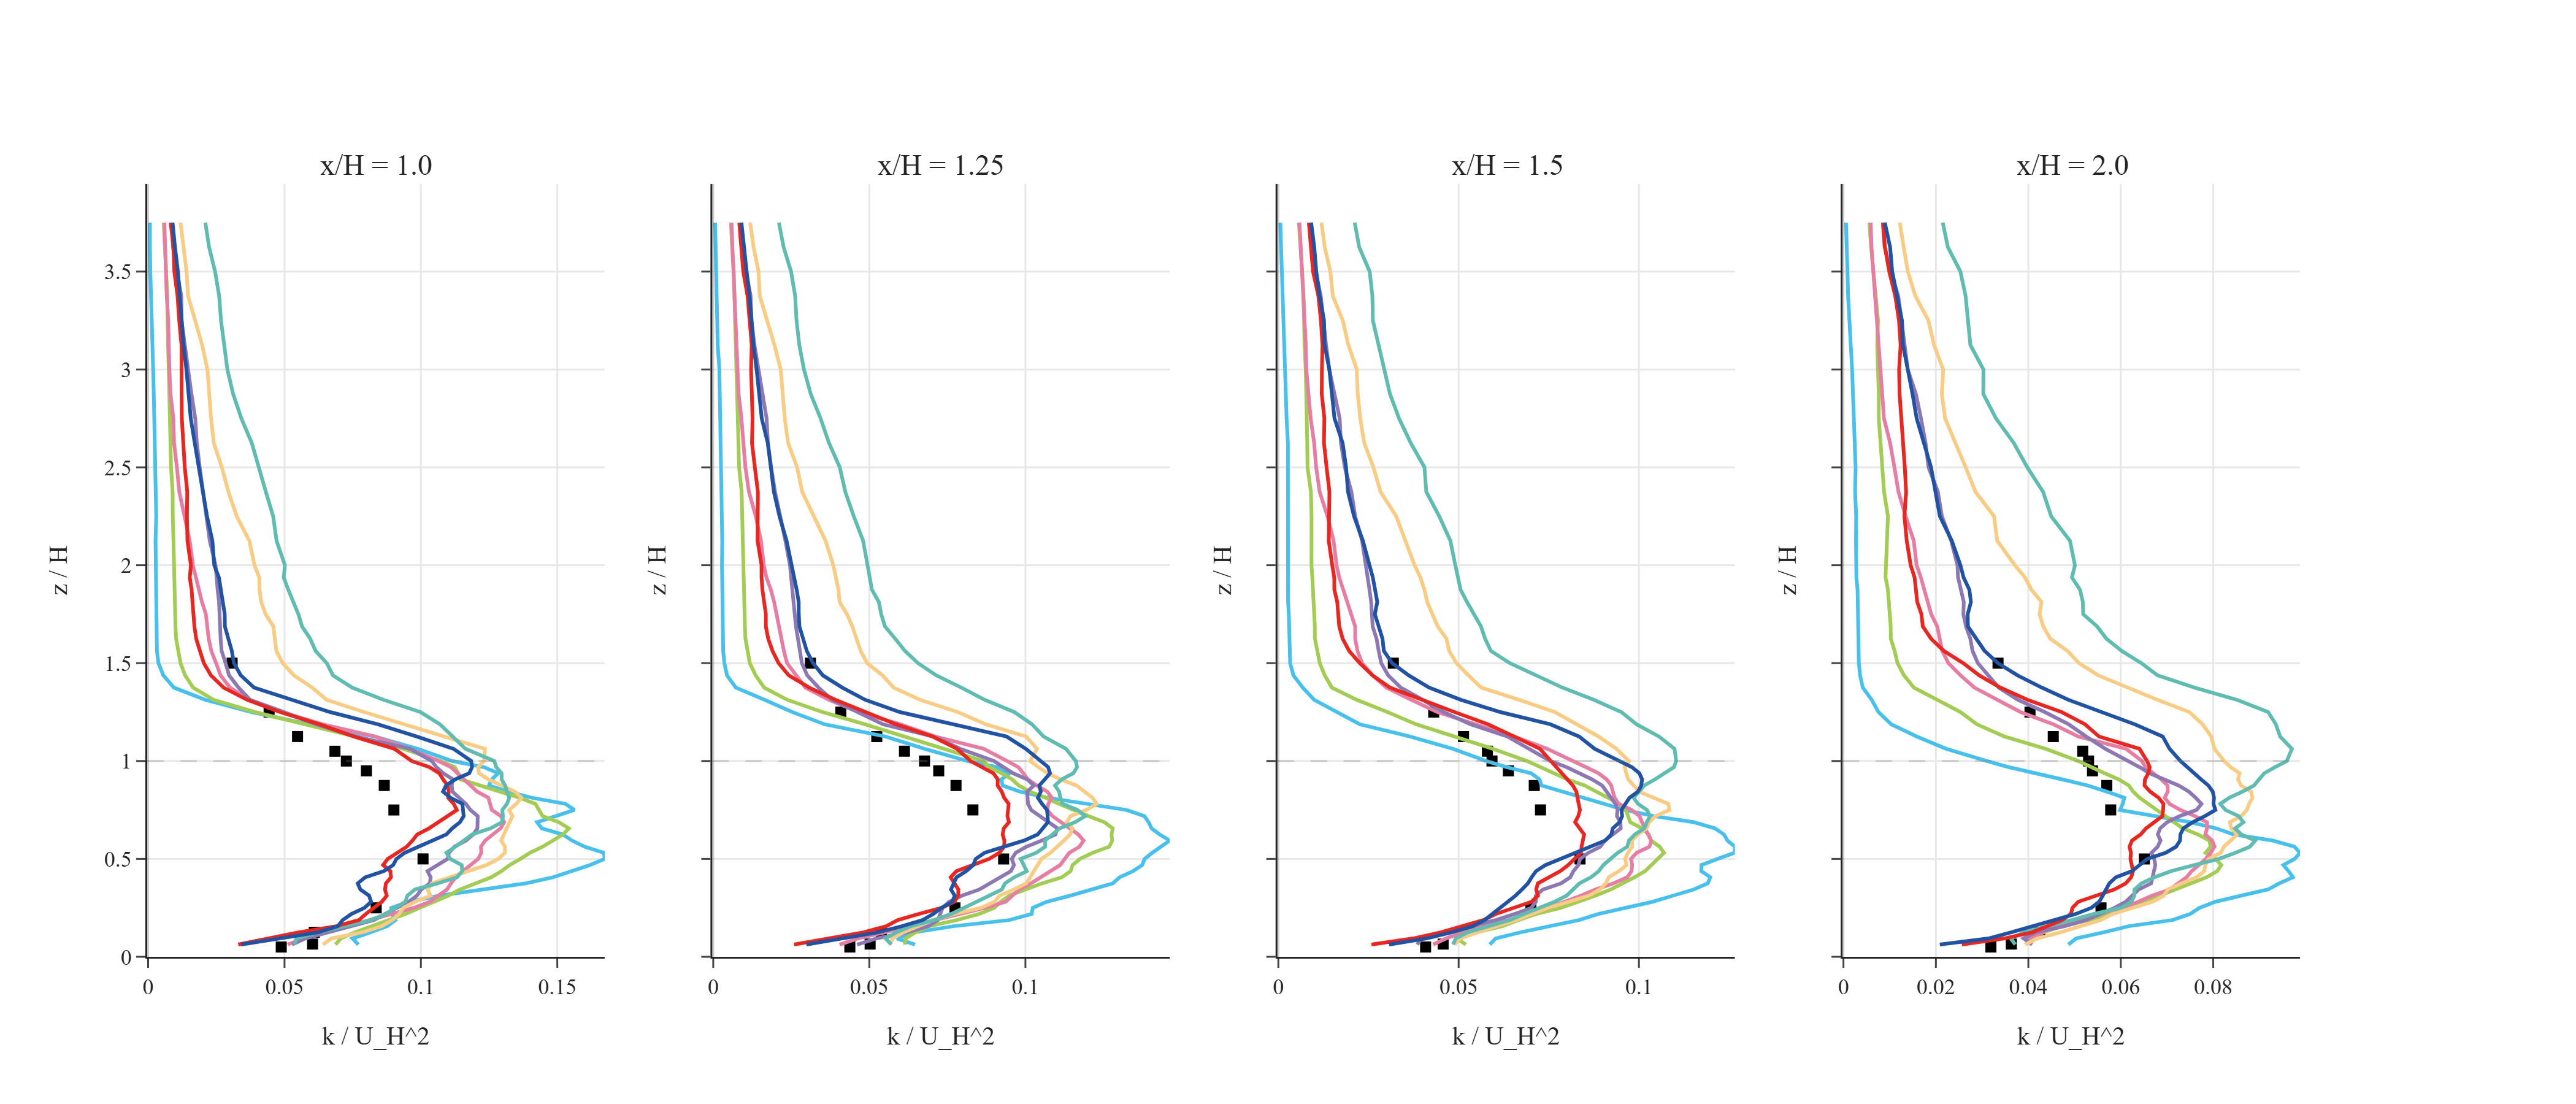
\includegraphics[width=0.85\textwidth]{figures/multi_case_comparisons_z0change/multi_case_comparison_TKE_part3.png}
        \caption{}
    \end{subfigure}
    \caption{Normalized Turbulent Kinetic Energy ($k/U_H^2$) profiles at (a) Upwind locations ($x/H < 0$), (b) Near Wake locations ($x/H \ge 0$), and (c) Far Wake locations.}
    \label{fig:results_tke}
\end{figure}

\autoref{fig:results_tke} presents the vertical profiles of the normalized Turbulent Kinetic Energy (TKE). As expected, the TKE profiles closely follow the trends observed in the $v_{rms}$ and $w_{rms}$ results, given that TKE is mathematically defined as half the sum of the variances of the velocity components, as defined in \autoref{eq:TKE}.

The profiles exhibit consistent patterns of underprediction in the low-roughness cases and overprediction in the high-roughness cases (Cases 5 and 6). While the absolute magnitudes are smaller than the individual RMS components, the structural characteristics—including the anomalous peaks observed in the no-approach case remain present. The strong similarity between the TKE, $v_{rms}$, and $w_{rms}$ profiles reinforces the conclusion that the turbulence in the wake is dominated by the lateral and vertical mixing energy. Once again, the medium-roughness configurations, specifically Cases 7 and 8, provide the most balanced representation of the TKE profiles, capturing the energy distribution with the highest degree of fidelity relative to the experimental benchmark.

\subsubsection{Validation of Wind and Turbulence Statistics}

\begin{figure}[htbp]
    \centering
    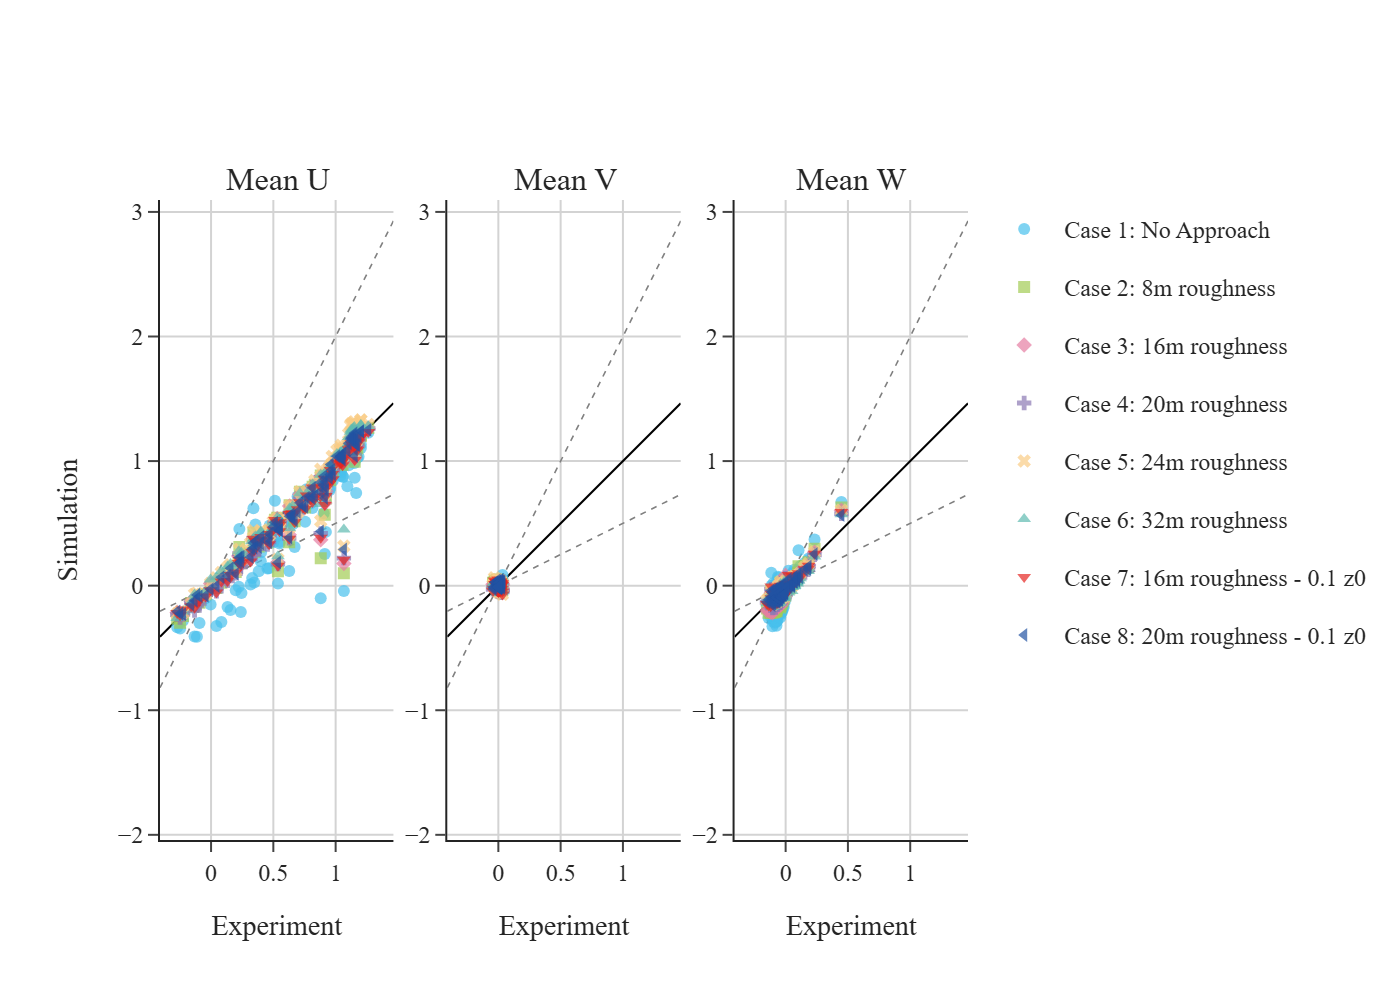
\includegraphics[width=0.85\textwidth]{figures/validation_plots_combined_z0change/combined_mean_velocities.png}
    \caption{Scatter plot comparison of normalized mean velocity components ($\bar{u}, \bar{v}, \bar{w}$) against AIJ experimental data across all cases. Solid lines represent the 1:1 correlation, while dashed lines indicate the $FAC2$ boundaries.}
    \label{fig:scatter_mean_velocities}
\end{figure}

\begin{figure}[htbp]
    \centering
    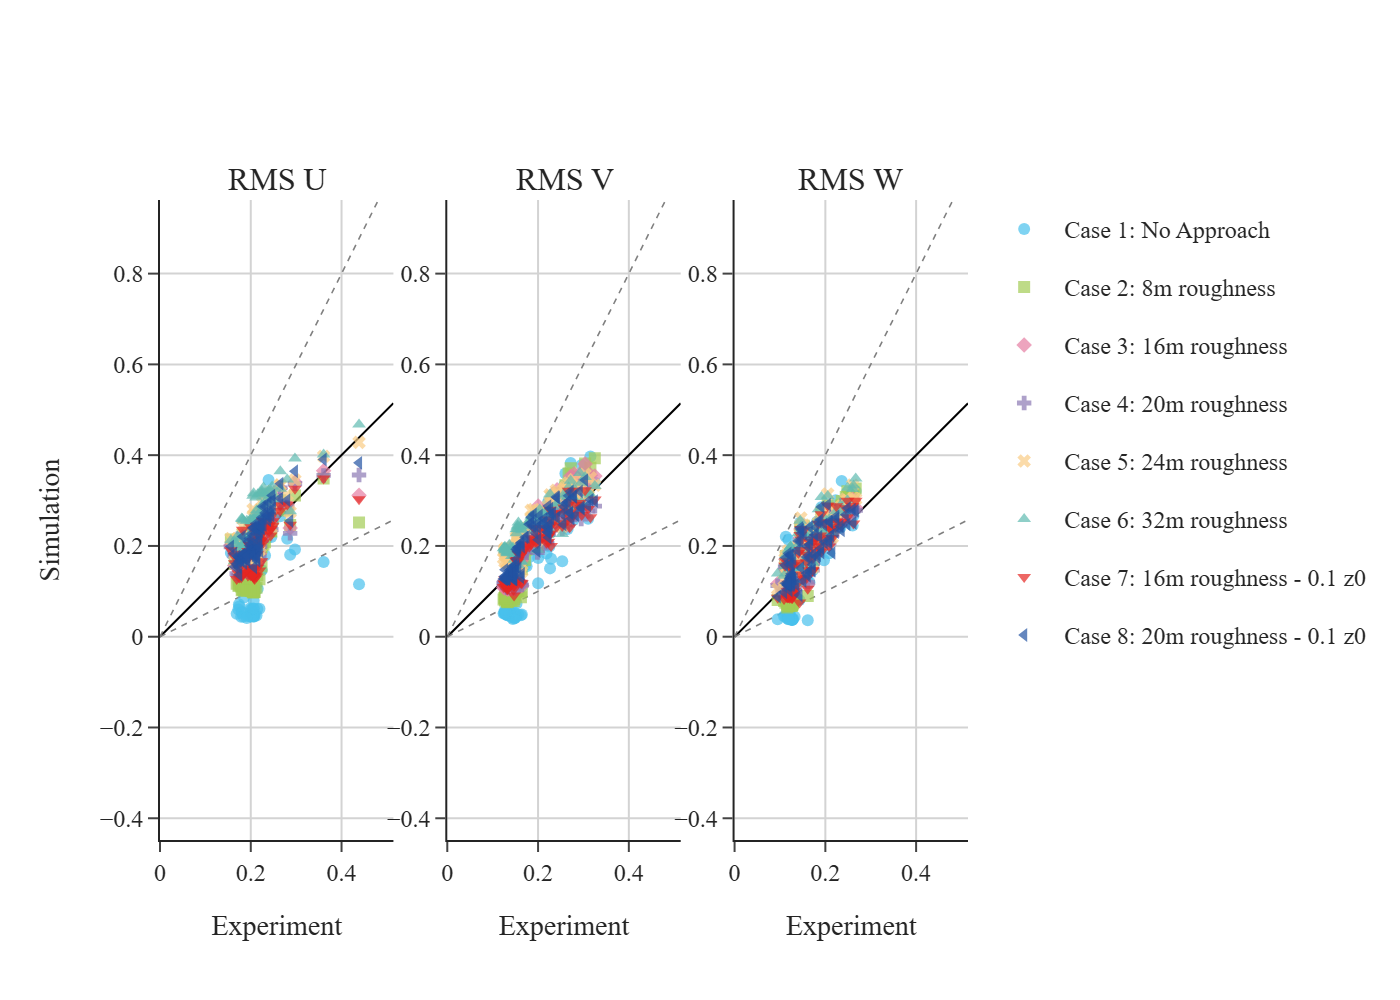
\includegraphics[width=0.85\textwidth]{figures/validation_plots_combined_z0change/combined_rms_velocities.png}
    \caption{Validation scatter plot for RMS velocity fluctuations ($u_{rms}, v_{rms}, w_{rms}$), demonstrating the solver's ability to capture turbulence intensity across the domain.}
    \label{fig:scatter_rms_velocities}
\end{figure}

\begin{figure}[htbp]
    \centering
    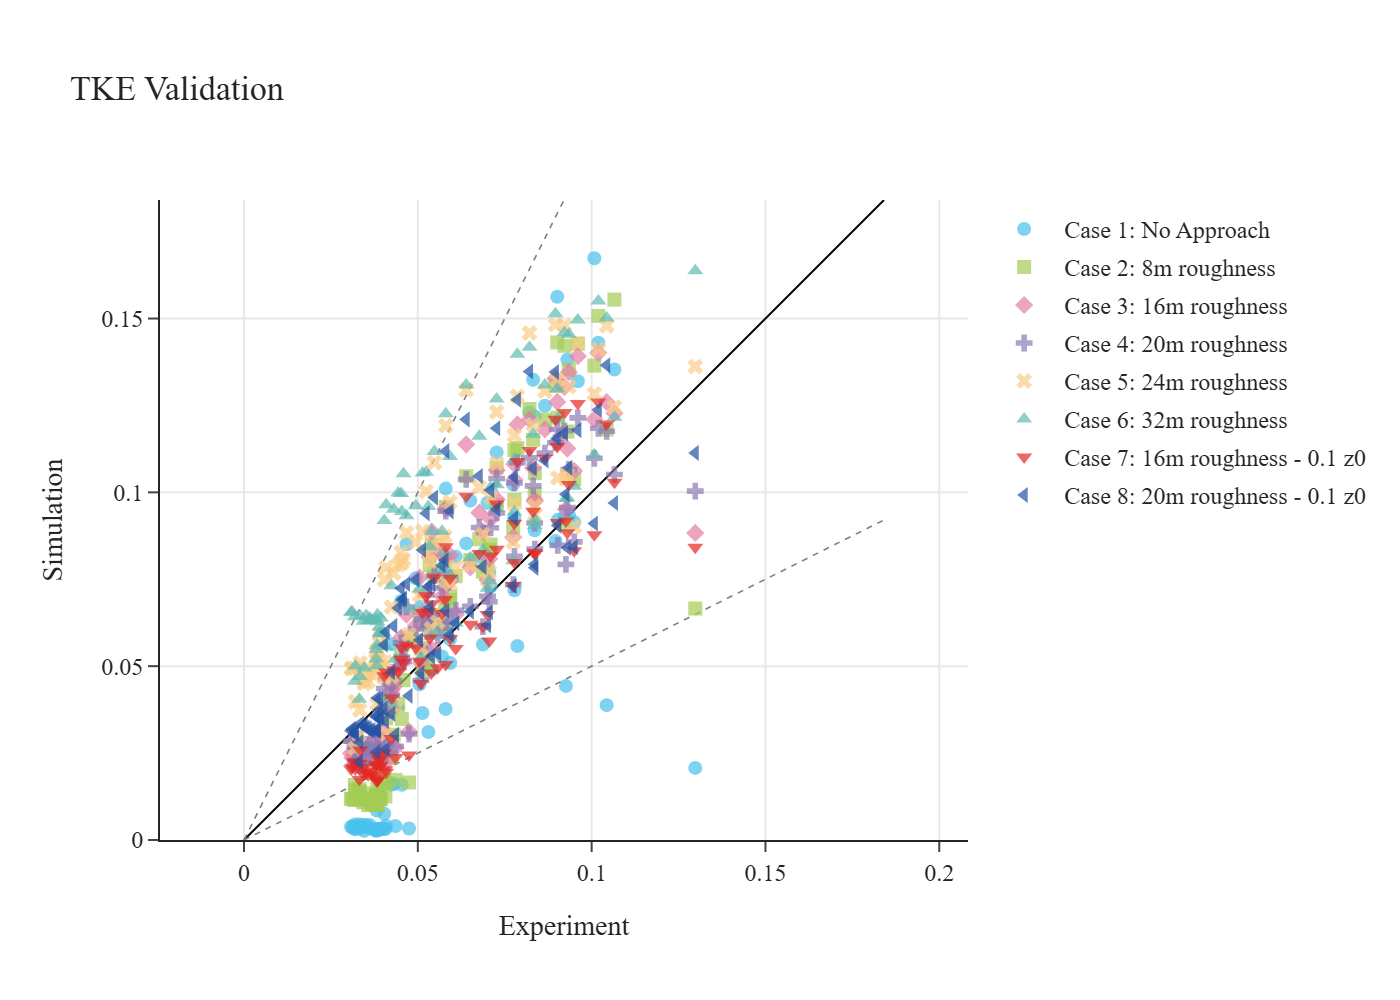
\includegraphics[width=0.85\textwidth]{figures/validation_plots_combined_z0change/combined_tke.png}
    \caption{Correlation of predicted vs. observed Turbulent Kinetic Energy ($k$), highlighting the impact of the refined $z_0$ and roughness configurations on energy modeling accuracy.}
    \label{fig:scatter_tke}
\end{figure}

\begin{table}[htbp]
    \centering
    \caption{Full validation results ($q$ and $FAC2$) for velocity components and turbulence metrics across all approach flow cases. Underlined values indicate performance below the standard thresholds ($q < 0.66$, $FAC2 < 0.50$).}
    \label{tab:full_validation_summary}
    \resizebox{\textwidth}{!}{
    \begin{tabular}{lcccccccccccccc}
        \toprule
        \textbf{Case} & \multicolumn{2}{c}{\textbf{$u$}} & \multicolumn{2}{c}{\textbf{$v$}} & \multicolumn{2}{c}{\textbf{$w$}} & \multicolumn{2}{c}{\textbf{$u_{rms}$}} & \multicolumn{2}{c}{\textbf{$v_{rms}$}} & \multicolumn{2}{c}{\textbf{$w_{rms}$}} & \multicolumn{2}{c}{\textbf{$TKE$}} \\
        \cmidrule(lr){2-3} \cmidrule(lr){4-5} \cmidrule(lr){6-7} \cmidrule(lr){8-9} \cmidrule(lr){10-11} \cmidrule(lr){12-13} \cmidrule(lr){14-15}
        & $q$ & $FAC2$ & $q$ & $FAC2$ & $q$ & $FAC2$ & $q$ & $FAC2$ & $q$ & $FAC2$ & $q$ & $FAC2$ & $q$ & $FAC2$ \\
        \midrule
        Case 1: No Approach & \underline{0.533} & 0.700 & 0.933 & 0.978 & \underline{0.389} & \underline{0.433} & \underline{0.622} & 0.622 & \underline{0.644} & 0.644 & \underline{0.611} & 0.667 & \underline{0.489} & 0.589 \\
        Case 2: 8m roughness & 0.900 & 0.956 & 0.933 & 0.989 & \underline{0.456} & 0.589 & 0.944 & 0.944 & 1.000 & 1.000 & 0.956 & 1.000 & \underline{0.611} & 0.678 \\
        Case 3: 16m roughness & 0.911 & 0.967 & 0.978 & 1.000 & \underline{0.533} & 0.567 & 1.000 & 1.000 & 1.000 & 1.000 & 0.956 & 1.000 & 0.933 & 1.000 \\
        Case 4: 20m roughness & 0.822 & 0.933 & 0.900 & 0.967 & \underline{0.567} & 0.600 & 1.000 & 1.000 & 1.000 & 1.000 & 1.000 & 1.000 & 0.978 & 1.000 \\
        Case 5: 24m roughness & 0.900 & 0.978 & 0.922 & 0.967 & 0.711 & 0.756 & 1.000 & 1.000 & 0.967 & 1.000 & 0.900 & 1.000 & \underline{0.656} & 0.978 \\
        Case 6: 32m roughness & 0.933 & 0.978 & 0.822 & 0.978 & \underline{0.578} & 0.633 & 0.978 & 1.000 & 0.867 & 1.000 & 0.856 & 1.000 & \underline{0.478} & 0.833 \\
        Case 7: 16m roughness - 0.1 z0 & 0.867 & 0.922 & 0.878 & 0.978 & 0.689 & 0.678 & 1.000 & 1.000 & 1.000 & 1.000 & 0.967 & 1.000 & 0.922 & 0.933 \\
        Case 8: 20m roughness - 0.1 z0 & 0.911 & 0.956 & 0.967 & 1.000 & 0.756 & 0.644 & 1.000 & 1.000 & 1.000 & 1.000 & 0.922 & 1.000 & 0.811 & 1.000 \\
        \bottomrule
    \end{tabular}
    }
\end{table}

The validation results highlight the critical role of approach flow modeling in the validation study.
While Case 1 (No Approach) consistently fails the $0.66$ hit-rate ($q$) threshold across several components, the introduction of surface roughness in Cases 2-8 brings the streamwise velocity ($u$) and fluctuation components ($u_{rms}$, $v_{rms}$, $w_{rms}$) into strong alignment with experimental standards.
Notably, vertical velocity ($w$) and Turbulent Kinetic Energy ($TKE$) remain the most sensitive parameters, occasionally falling below the standard in lower-roughness scenarios, but showing marked improvement as roughness height increases.
This suggests that the LBM solver combined with the TSUBAME 4.0 is highly capable of capturing complex urban wind fields, provided the inflow turbulence is correctly parameterized.

\begin{table}[htbp]
    \centering
    \caption{MAE and RMSE validation metrics for velocity components and TKE across all approach flow cases.}
    \label{tab:mae_rmse_validation}
    \resizebox{\textwidth}{!}{
    \begin{tabular}{lcccccccccccccc}
        \toprule
        \textbf{Case} & \multicolumn{2}{c}{\textbf{$u$}} & \multicolumn{2}{c}{\textbf{$v$}} & \multicolumn{2}{c}{\textbf{$w$}} & \multicolumn{2}{c}{\textbf{$u_{rms}$}} & \multicolumn{2}{c}{\textbf{$v_{rms}$}} & \multicolumn{2}{c}{\textbf{$w_{rms}$}} & \multicolumn{2}{c}{\textbf{$TKE$}} \\
        \cmidrule(lr){2-3} \cmidrule(lr){4-5} \cmidrule(lr){6-7} \cmidrule(lr){8-9} \cmidrule(lr){10-11} \cmidrule(lr){12-13} \cmidrule(lr){14-15}
        & MAE & RMSE & MAE & RMSE & MAE & RMSE & MAE & RMSE & MAE & RMSE & MAE & RMSE & MAE & RMSE \\
        \midrule
        Case 1: No Approach & 0.2009 & 0.2726 & 0.0202 & 0.0267 & 0.0979 & 0.1212 & 0.0759 & 0.0996 & 0.0585 & 0.0675 & 0.0539 & 0.0619 & 0.0268 & 0.0320 \\
        Case 2: 8m roughness & 0.0751 & 0.1518 & 0.0171 & 0.0232 & 0.0585 & 0.0705 & 0.0438 & 0.0575 & 0.0433 & 0.0485 & 0.0394 & 0.0450 & 0.0220 & 0.0254 \\
        Case 3: 16m roughness & 0.0600 & 0.1286 & 0.0133 & 0.0184 & 0.0548 & 0.0650 & 0.0243 & 0.0304 & 0.0354 & 0.0407 & 0.0289 & 0.0341 & 0.0172 & 0.0208 \\
        Case 4: 20m roughness & 0.0690 & 0.1266 & 0.0271 & 0.0321 & 0.0461 & 0.0538 & 0.0232 & 0.0296 & 0.0218 & 0.0259 & 0.0261 & 0.0307 & 0.0123 & 0.0150 \\
        Case 5: 24m roughness & 0.0698 & 0.1194 & 0.0248 & 0.0304 & 0.0354 & 0.0429 & 0.0289 & 0.0366 & 0.0466 & 0.0518 & 0.0408 & 0.0471 & 0.0236 & 0.0286 \\
        Case 6: 32m roughness & 0.0527 & 0.0925 & 0.0290 & 0.0338 & 0.0419 & 0.0501 & 0.0447 & 0.0537 & 0.0470 & 0.0537 & 0.0463 & 0.0524 & 0.0294 & 0.0348 \\
        Case 7: 16m roughness - 0.1 z0 & 0.0843 & 0.1398 & 0.0247 & 0.0317 & 0.0387 & 0.0459 & 0.0304 & 0.0401 & 0.0215 & 0.0251 & 0.0310 & 0.0366 & 0.0135 & 0.0161 \\
        Case 8: 20m roughness - 0.1 z0 & 0.0714 & 0.1238 & 0.0145 & 0.0184 & 0.0364 & 0.0415 & 0.0241 & 0.0291 & 0.0256 & 0.0328 & 0.0269 & 0.0377 & 0.0149 & 0.0206 \\
        \bottomrule
    \end{tabular}
    }
\end{table}

The quantitative assessment of the error metrics further supports the conclusions drawn from the hit rate analysis. In Case 1, the RMSE for streamwise velocity $u$ is notably high at 0.2726, representing a significant deviation from experimental values. However, across the roughness-modified Cases 2-8, the RMSE for $u$ is reduced by over 50\% in most instances, reaching its minimum in Case 6 (0.0925). Interestingly, the vertical velocity components ($v, w$) and turbulence fluctuations show relatively stable and low MAE values ($< 0.05$) across the majority of the cases. The $TKE$ errors are particularly low in the optimized roughness scenarios (e.g., Case 4 with an RMSE of 0.0150), demonstrating that the solver's ability to capture the energy distribution within the flow field is highly dependent on the correct specification of the approach flow boundary layer. These low absolute errors confirm that the model's predictions are not only statistically correlated but also physically accurate in magnitude.

\subsection{Particle Concentration}
\subsubsection{Particle Concentration Profile}

\begin{figure}[htbp]
    \centering
    \begin{subfigure}[b]{\textwidth}
        \centering
        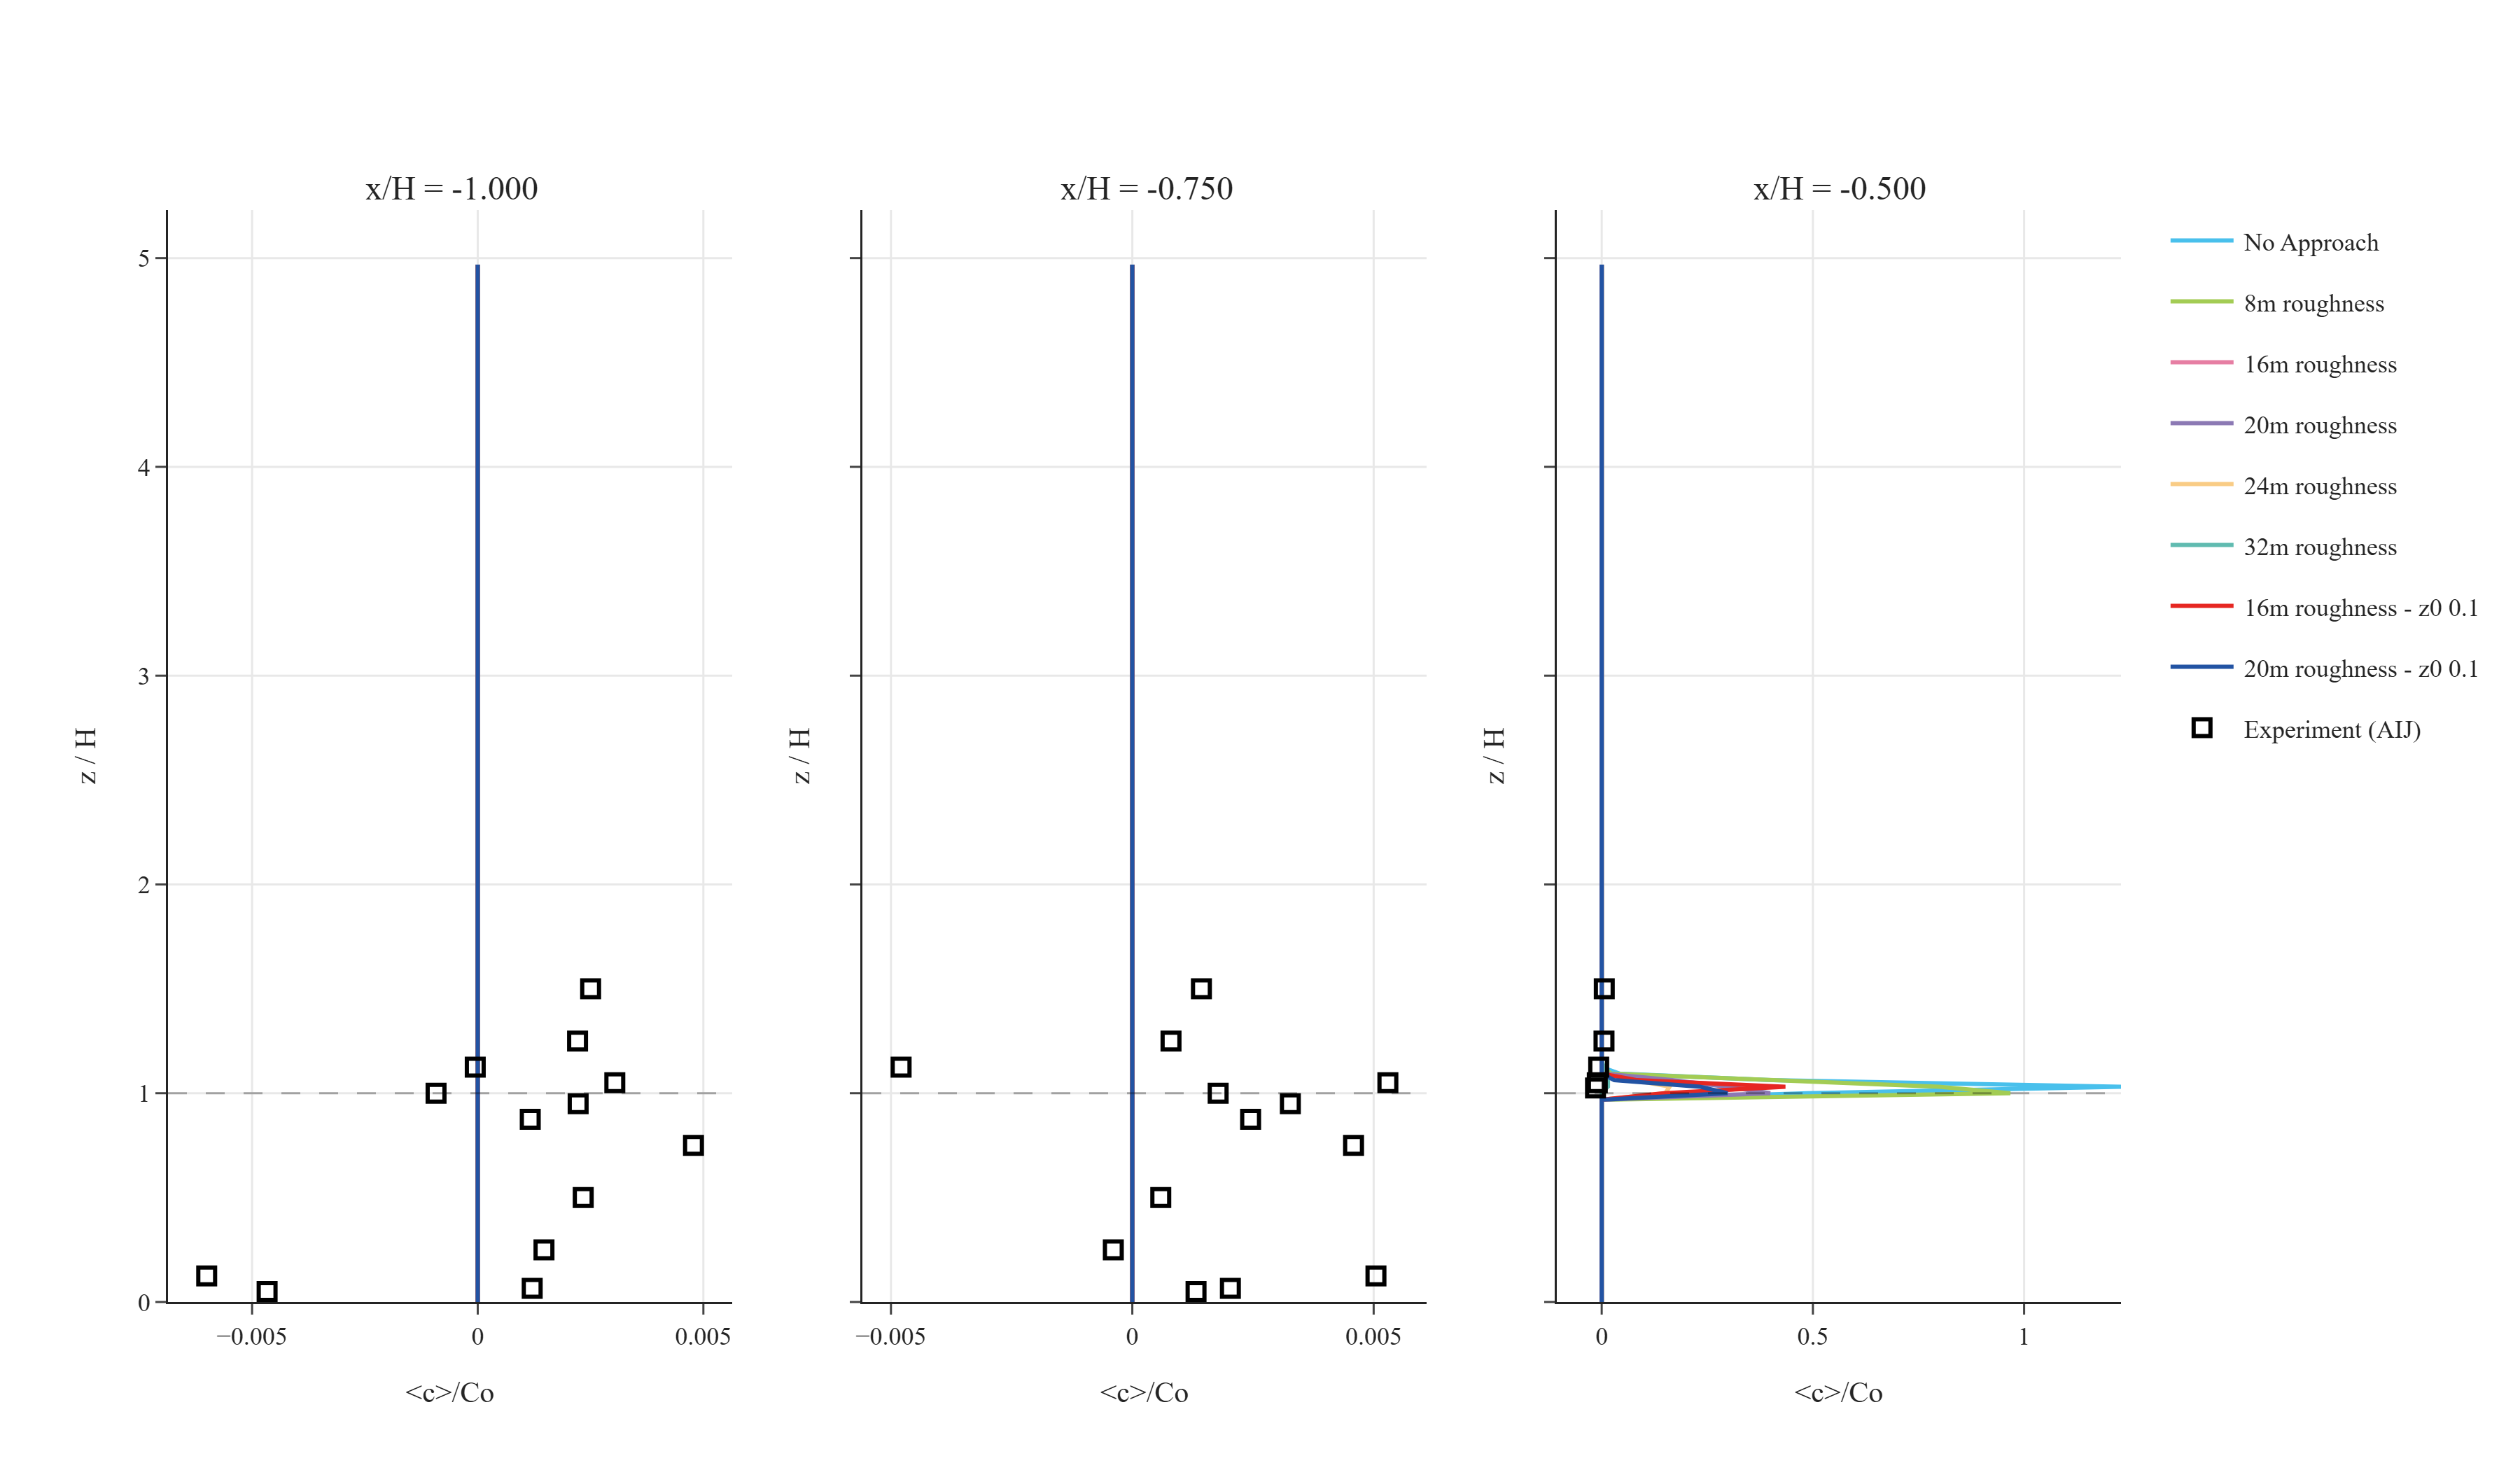
\includegraphics[width=0.85\textwidth]{figures/concentration_comparison/multi_case_comparison_part1.png}
        \caption{}
    \end{subfigure}
    \vspace{1ex}
    \begin{subfigure}[b]{\textwidth}
        \centering
        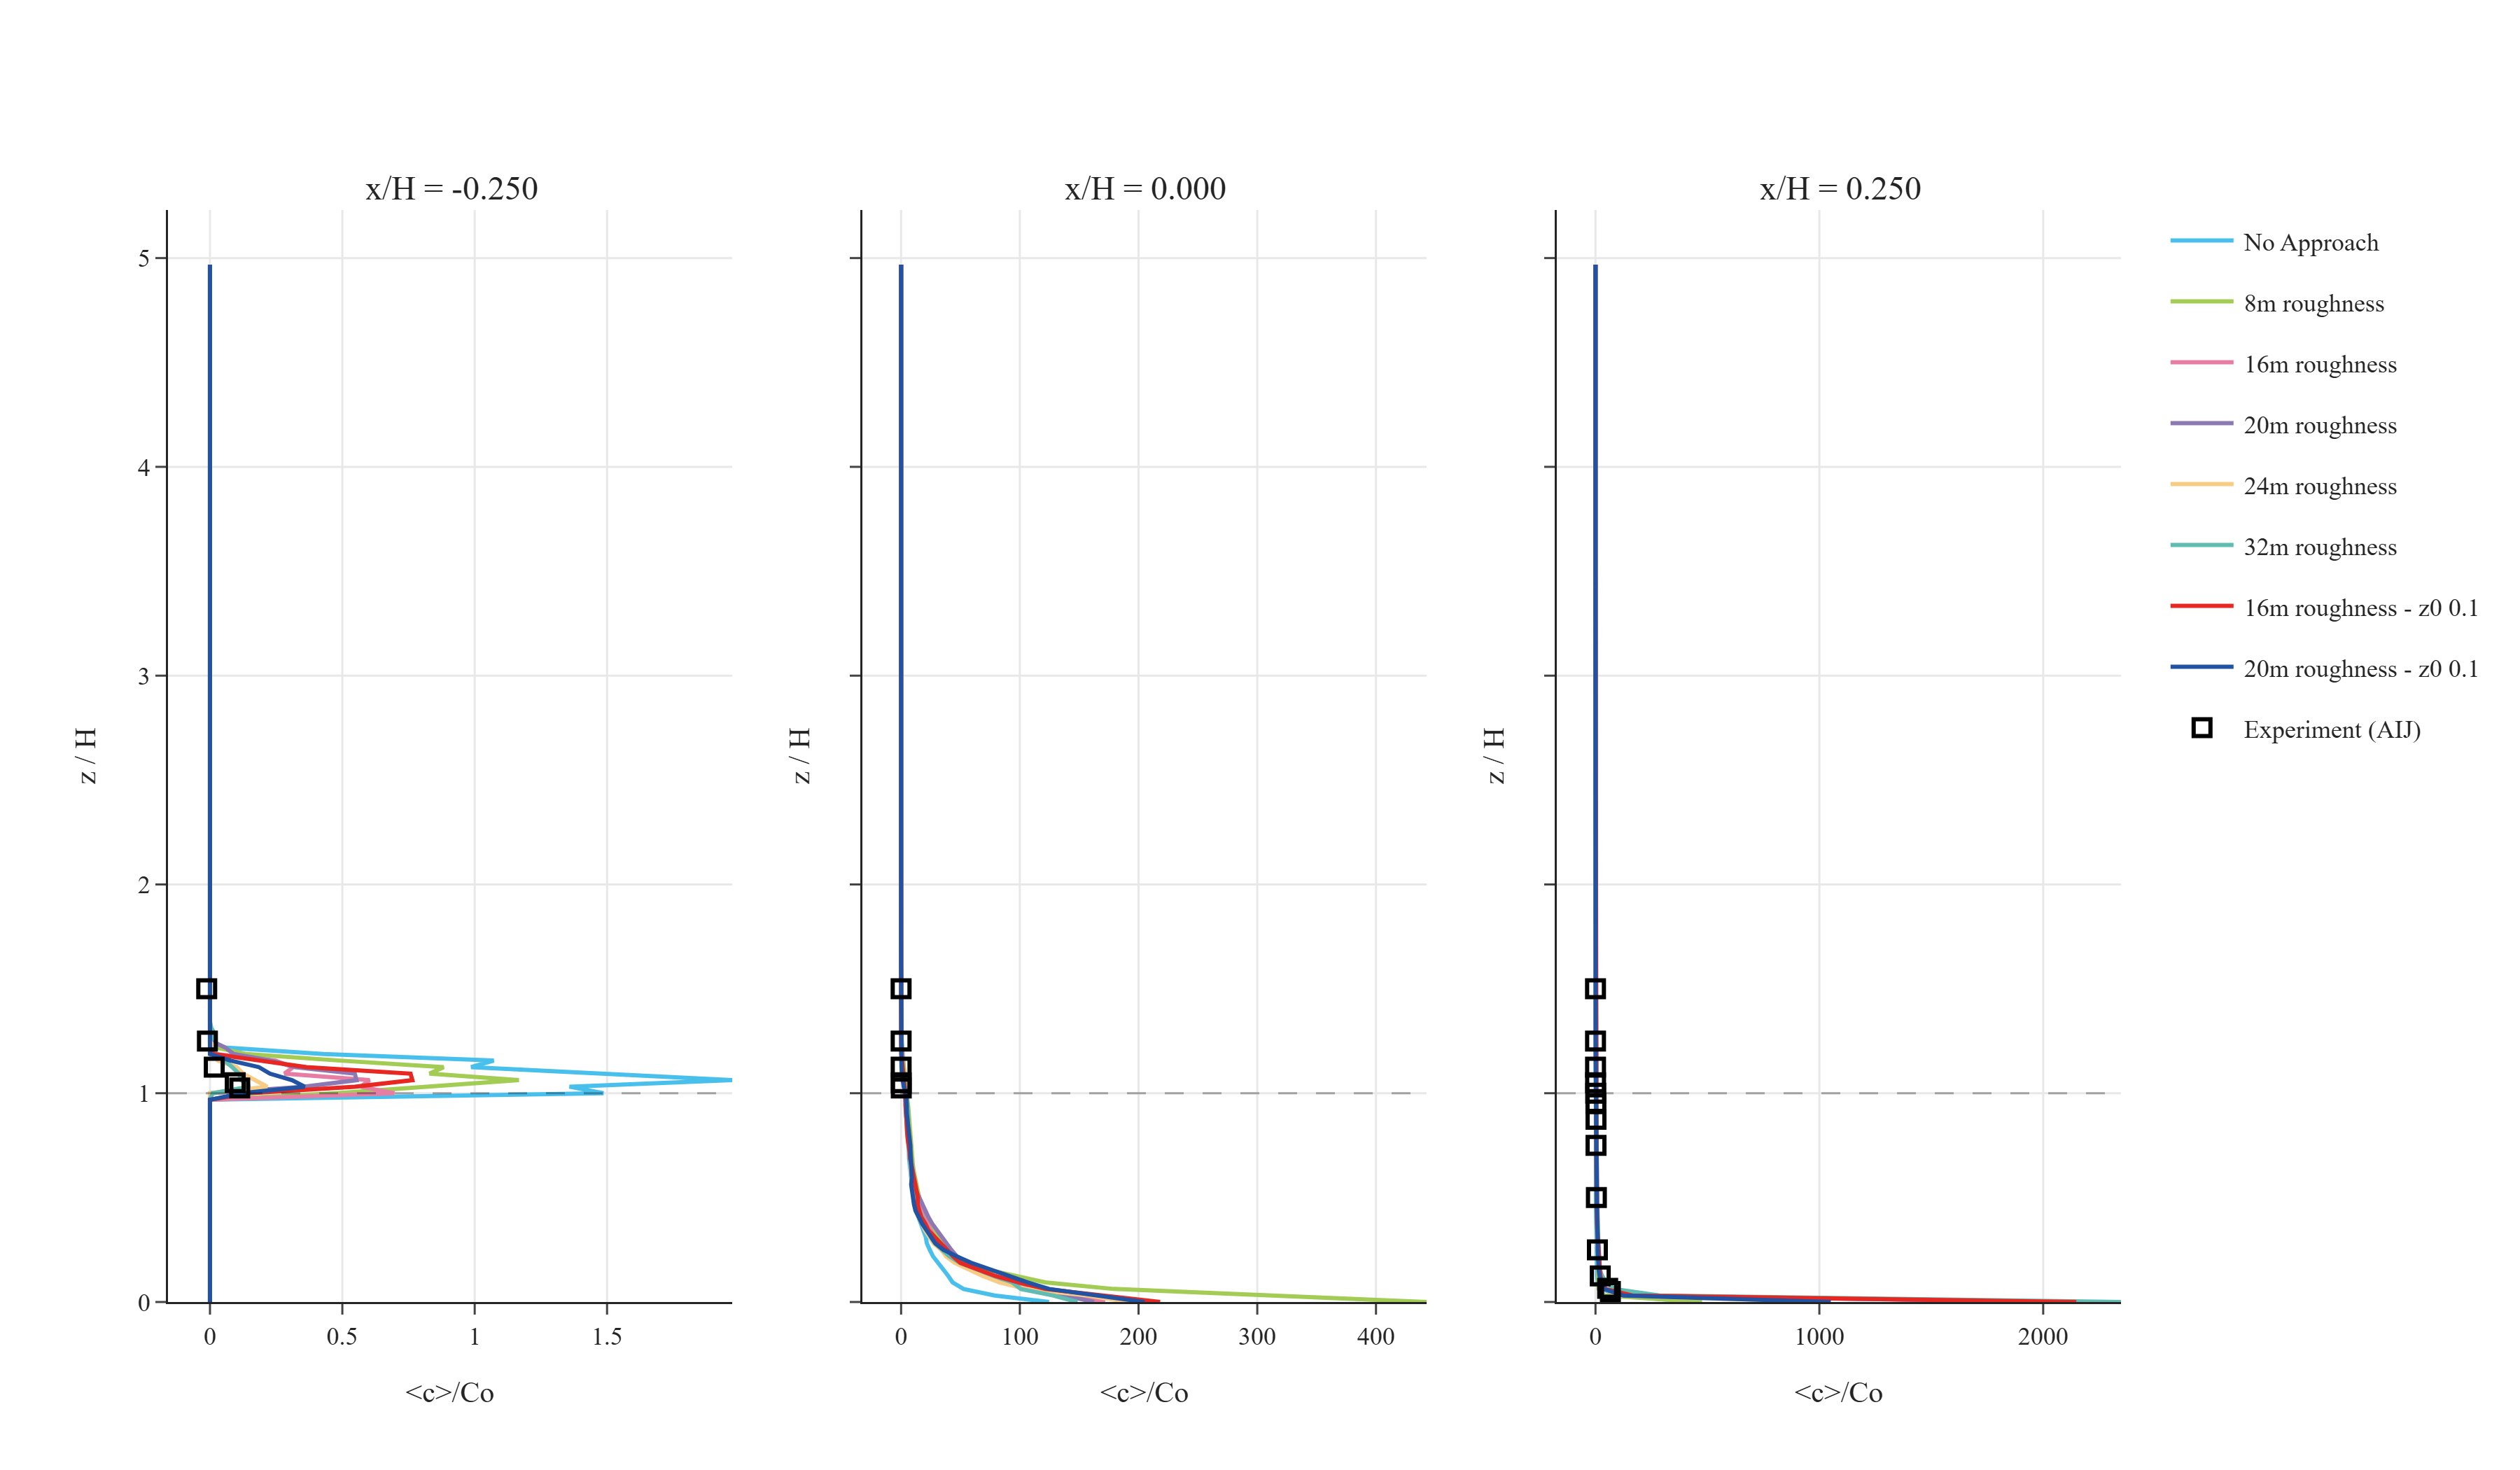
\includegraphics[width=0.85\textwidth]{figures/concentration_comparison/multi_case_comparison_part2.png}
        \caption{}
    \end{subfigure}
    \vspace{1ex}
    \begin{subfigure}[b]{\textwidth}
        \centering
        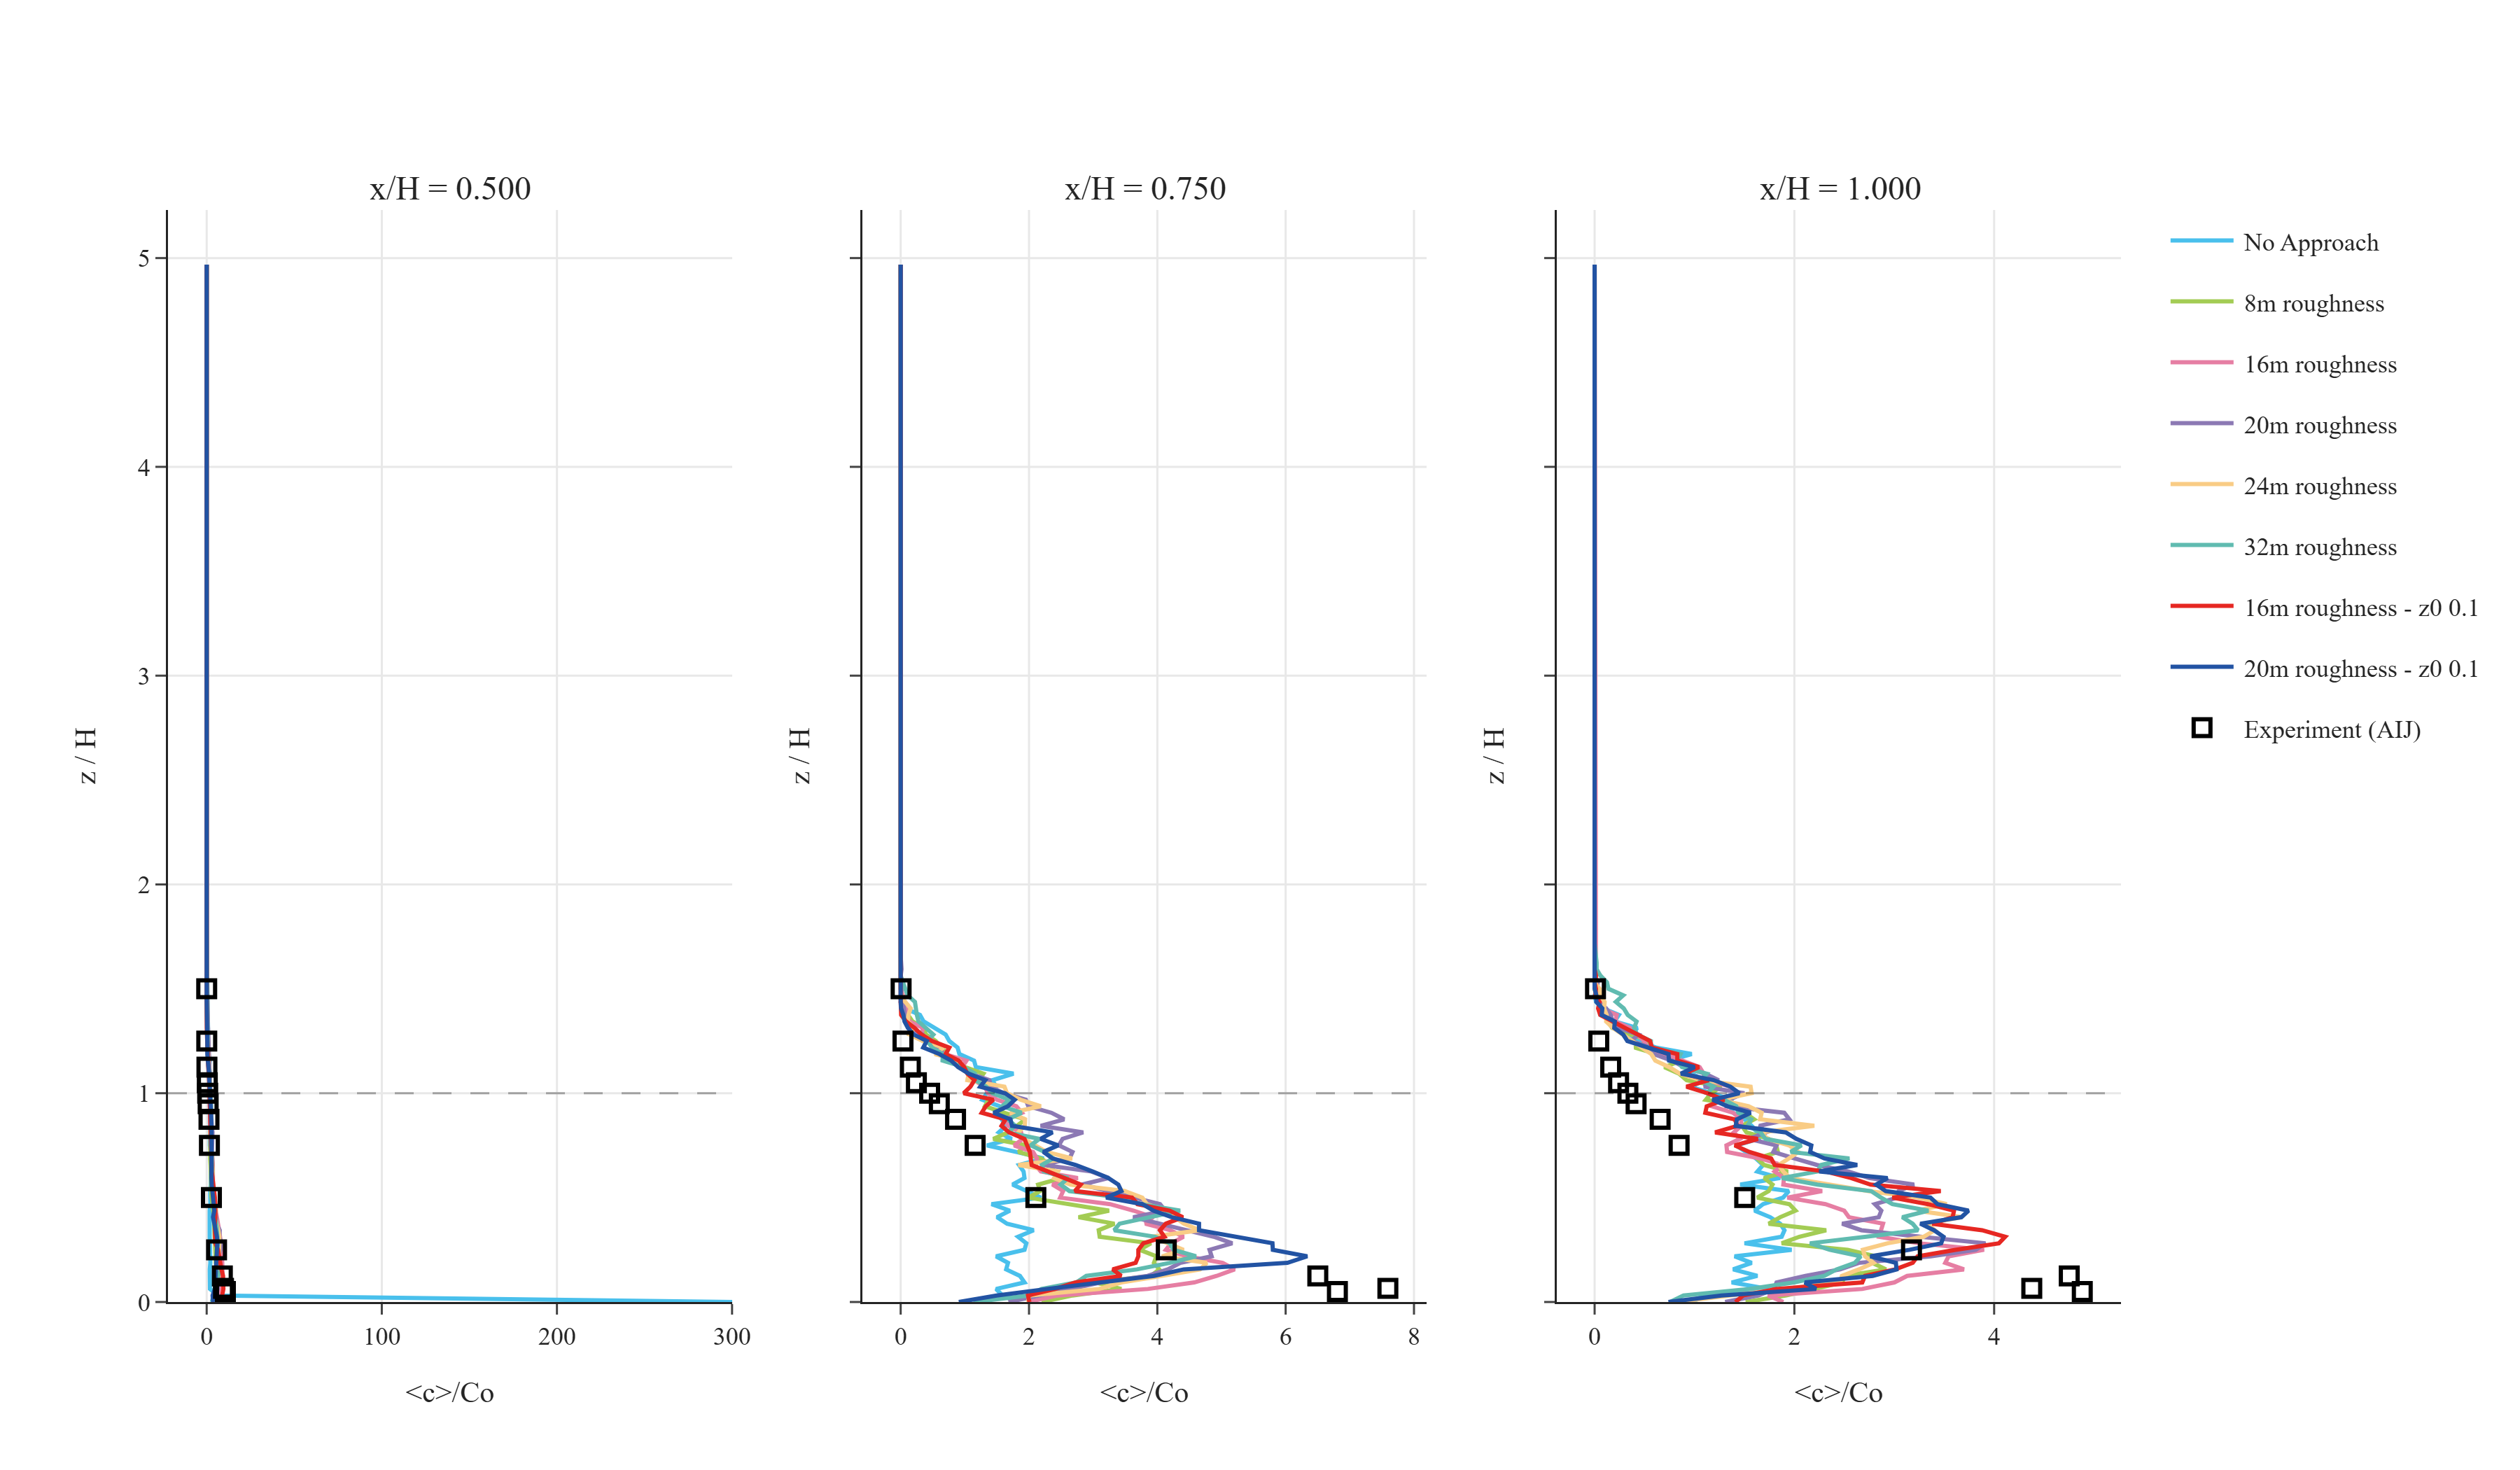
\includegraphics[width=0.85\textwidth]{figures/concentration_comparison/multi_case_comparison_part3.png}
        \caption{}
    \end{subfigure}
    \vspace{1ex}
    \begin{subfigure}[b]{\textwidth}
        \centering
        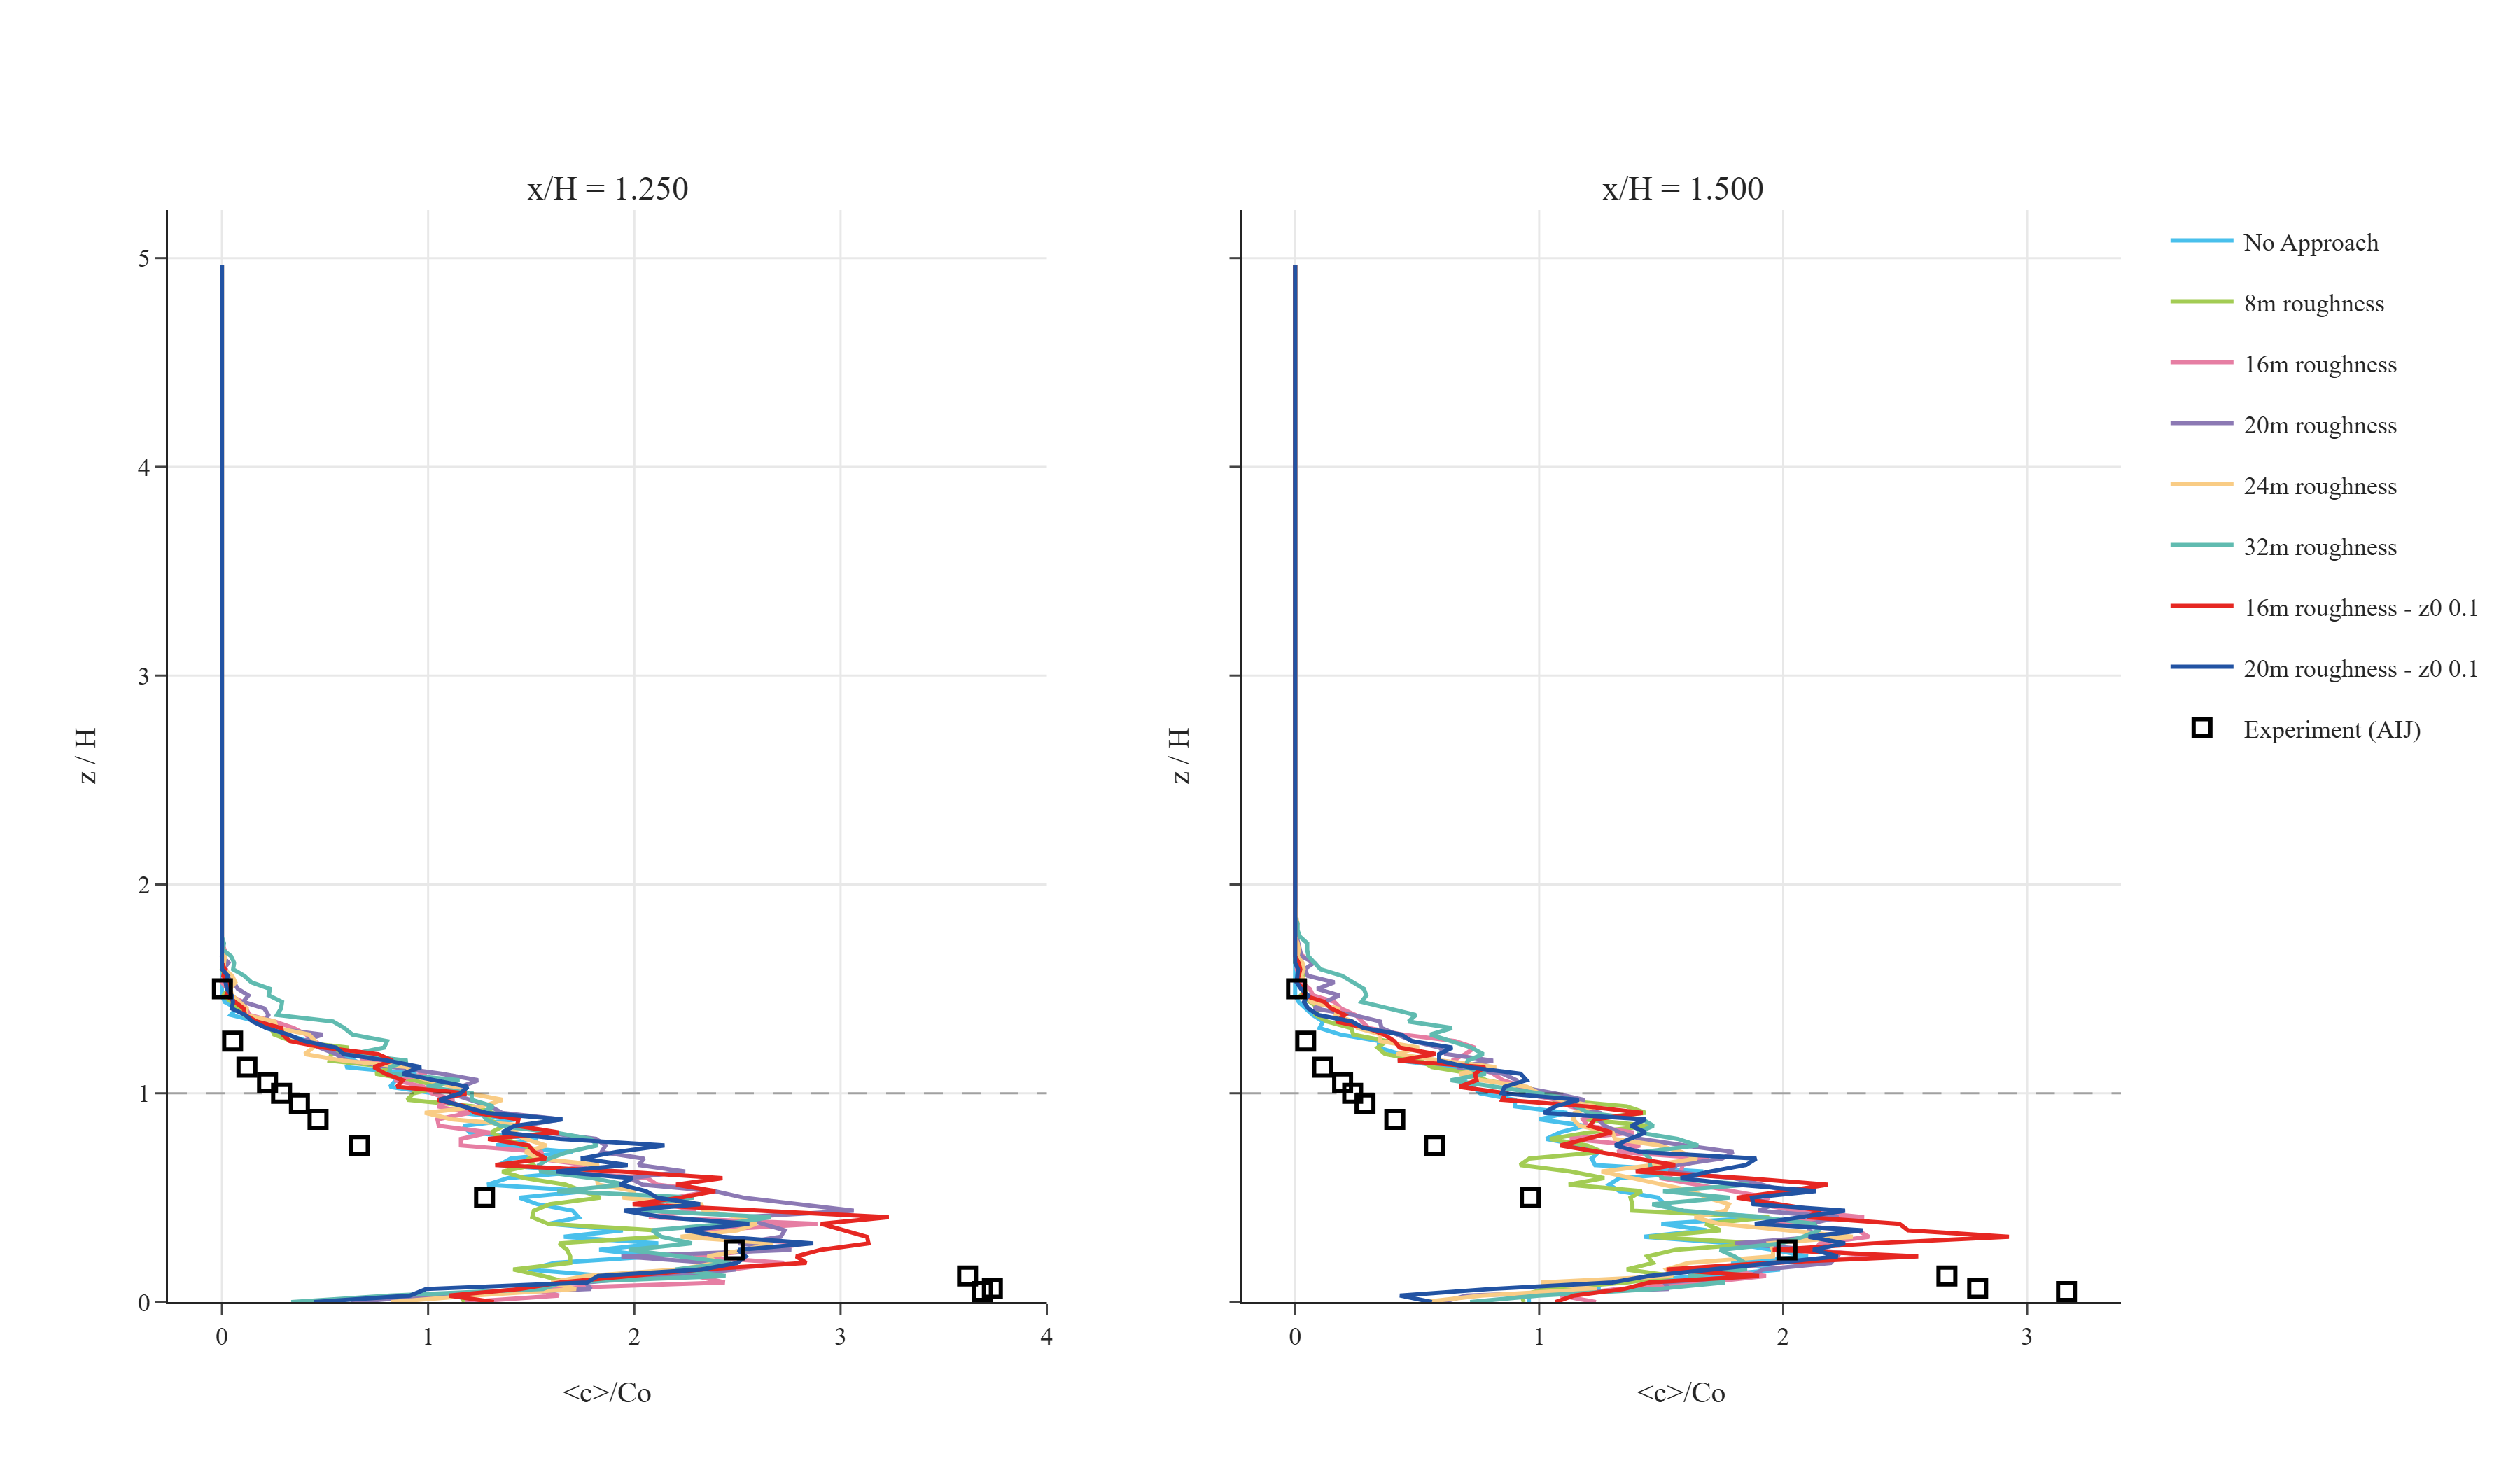
\includegraphics[width=0.85\textwidth]{figures/concentration_comparison/multi_case_comparison_part4.png}
        \caption{}
    \end{subfigure}
    \caption{Normalized concentration ($C_{norm}$) profiles at (a) Part 1, (b) Part 2, (c) Part 3, and (d) Part 4. The profiles illustrate the pollutant dispersion characteristics across the 12 AIJ measurement locations.}
    \label{fig:concentration_profiles_vertical}
\end{figure}

\subsubsection{Validation of Particle Concentration}

\begin{figure}[htbp]
    \centering
    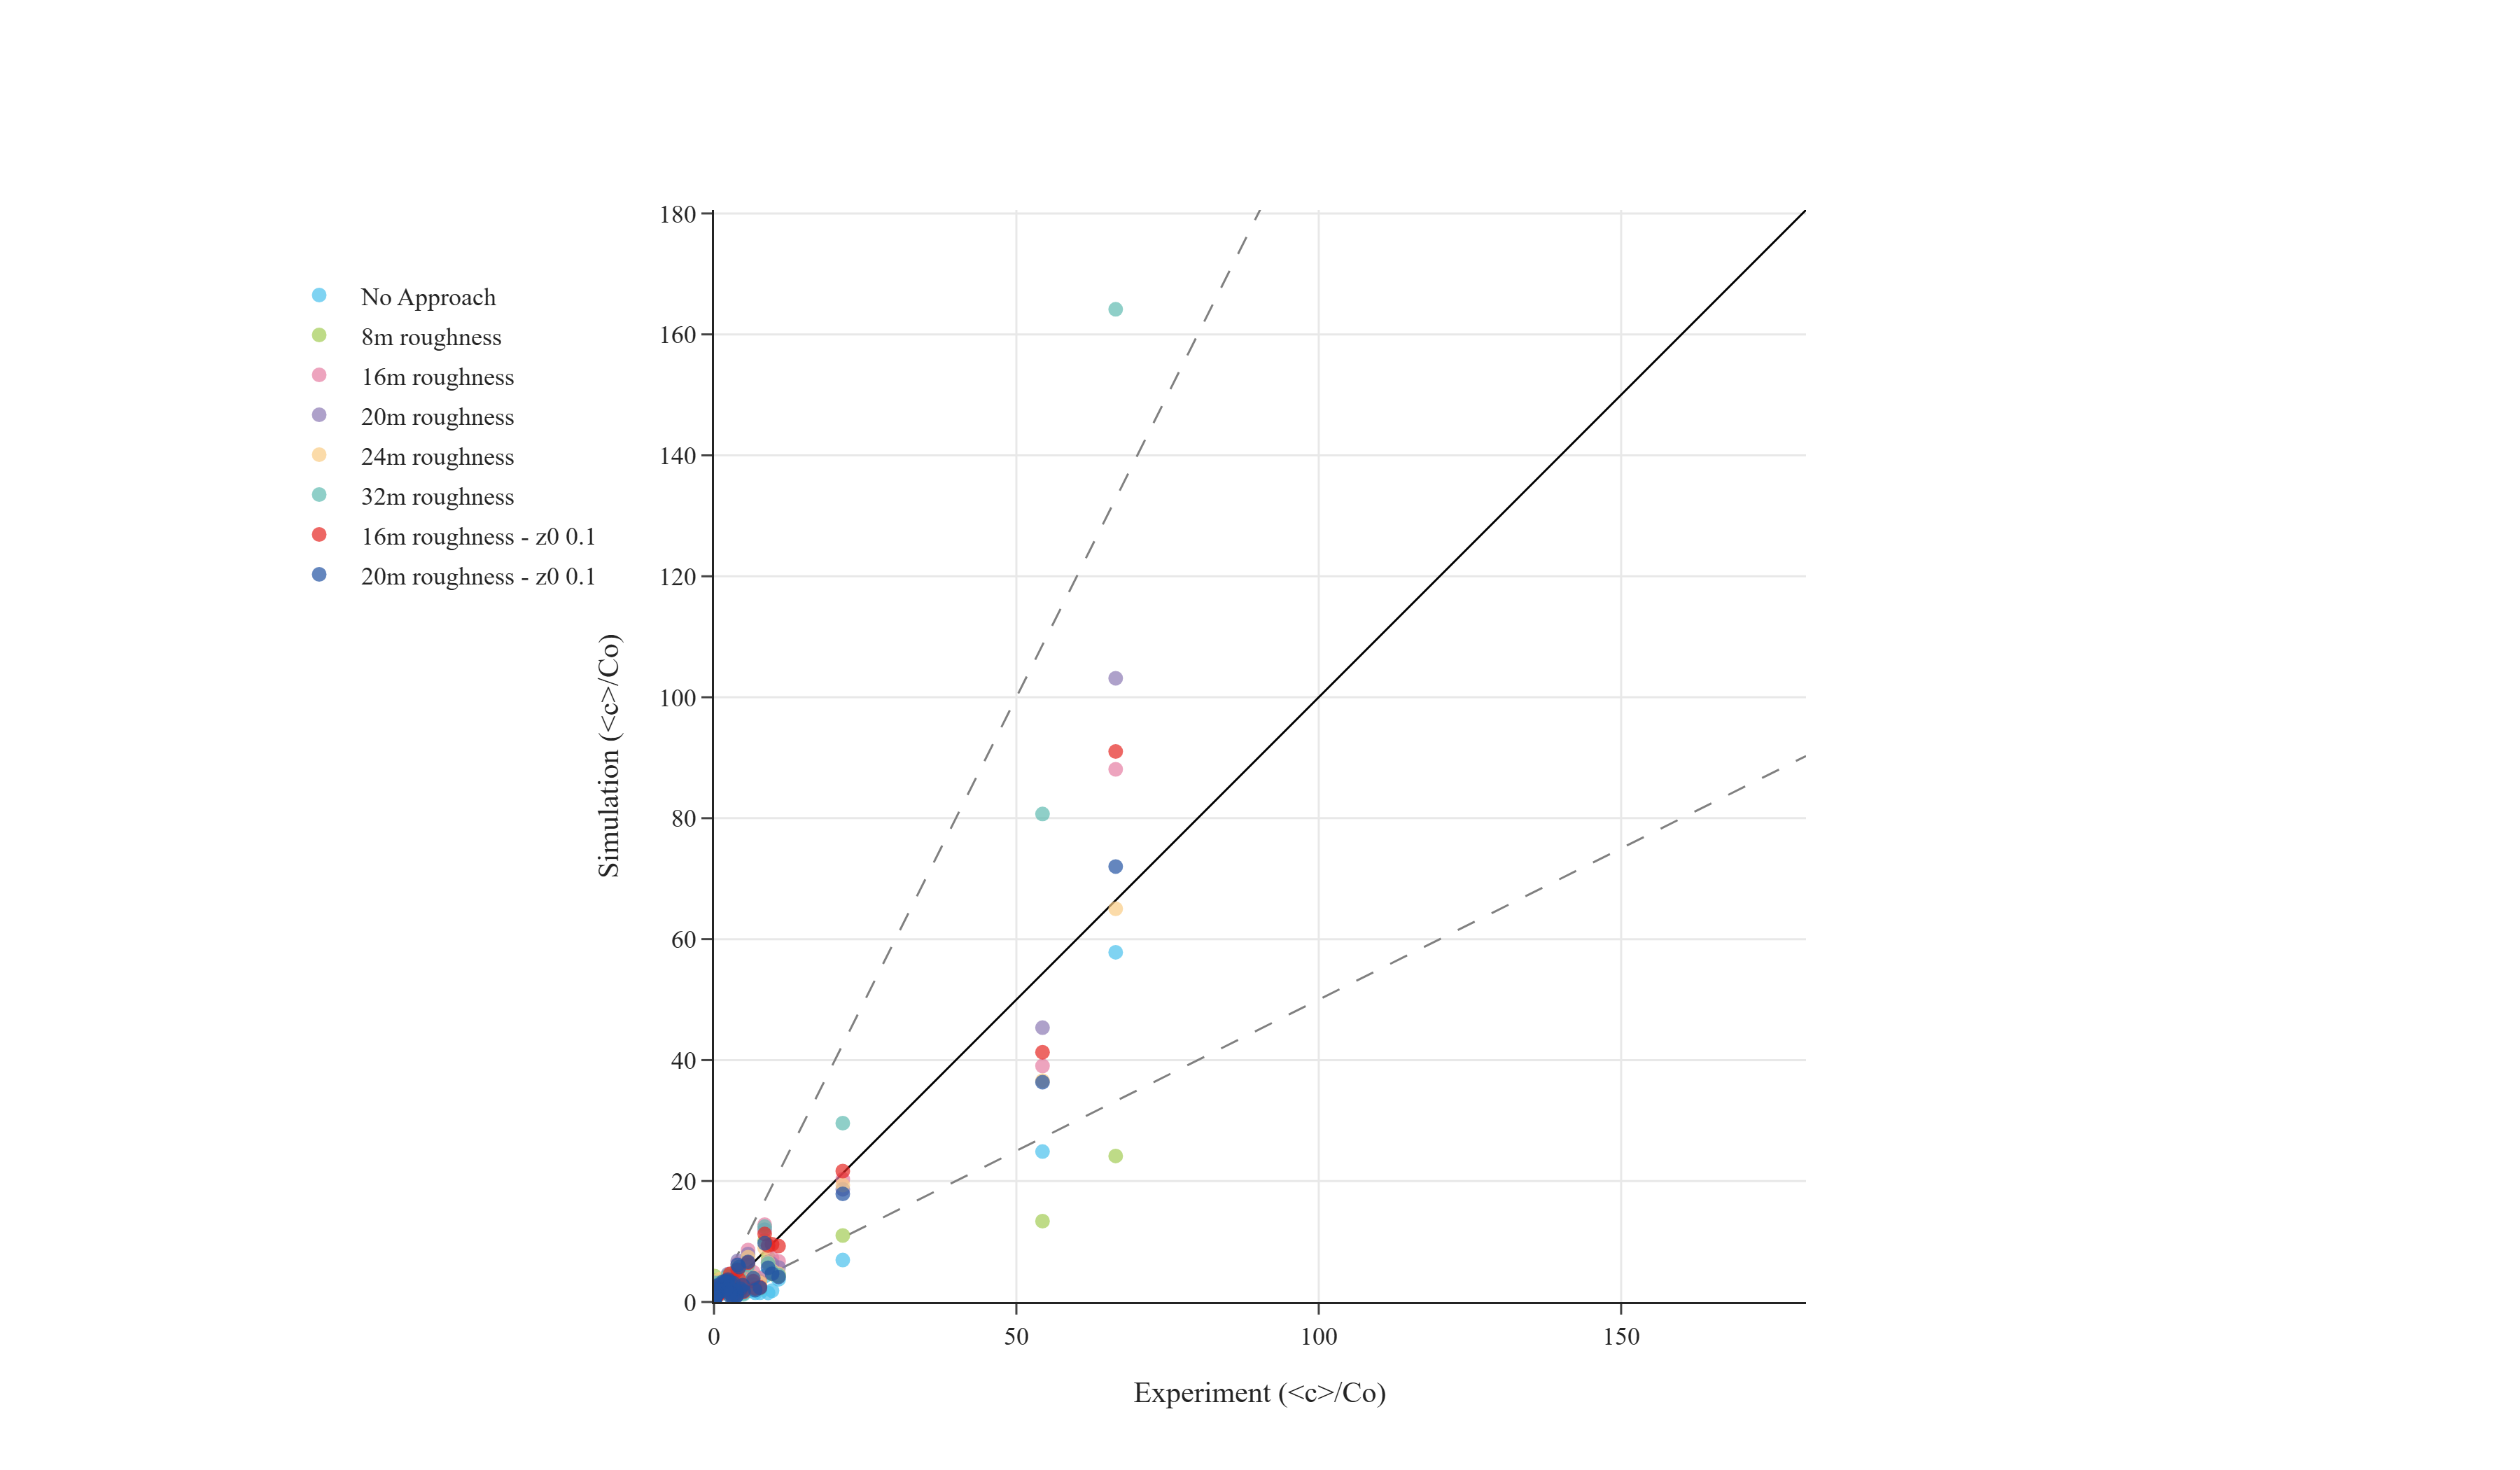
\includegraphics[width=0.85\textwidth]{figures/concentration_comparison/validation_scatter.png}
    \caption{Scatter plot comparison of normalized concentration ($C_{norm}$) results against AIJ experimental data. The solid line indicates the 1:1 ideal correlation, while the dashed lines represent the $FAC2$ boundaries.}
    \label{fig:concentration_validation_scatter}
\end{figure}

\begin{table}[htbp]
    \centering
    \caption{Concentration validation metrics across all approach flow cases. Underlined values indicate performance below the standard thresholds ($q < 0.66$, $FAC2 < 0.50$).}
    \label{tab:concentration_validation}
    \begin{tabular}{lccccc}
        \toprule
        \textbf{Case} & \textbf{N} & \textbf{$q$} & \textbf{FAC2} & \textbf{MAE} & \textbf{RMSE} \\
        \midrule
        No Approach            & 119 & \underline{0.387} & \underline{0.496} & 1.4737 & 3.6180 \\
        8m roughness           & 119 & \underline{0.403} & 0.513 & 1.6328 & 5.6510 \\
        16m roughness          & 119 & \underline{0.395} & 0.588 & 1.0878 & 2.7165 \\
        20m roughness          & 119 & \underline{0.353} & 0.504 & 1.3134 & 3.7468 \\
        24m roughness          & 119 & \underline{0.387} & 0.538 & 1.0368 & 2.1463 \\
        32m roughness          & 119 & \underline{0.353} & 0.529 & 2.0231 & 9.4304 \\
        16m roughness (z0 0.1) & 119 & \underline{0.420} & 0.605 & 1.0131 & 2.7927 \\
        20m roughness (z0 0.1) & 119 & \underline{0.395} & 0.538 & 1.1069 & 2.2813 \\
        \bottomrule
    \end{tabular}
\end{table}

The concentration validation results show a marked contrast to the velocity validation, with significantly lower accuracy across all metrics. For all simulation cases, the hit rate ($q$) remains well below the $0.66$ standard, peaking at only 0.420 in Case 7. While the $FAC2$ values mostly meet the $0.50$ threshold (with the exception of the "No Approach" baseline), they are considerably lower than the scores achieved for the flow field. These results suggest that the current Lagrangian particle tracker (LPT) within the LBM solver may not yet fully capture the complex dispersion characteristics of pollutants in an urban environment. This discrepancy could be attributed to the simplified physical modeling of generic particles in the solver, whereas the experimental data were collected using gases that exhibit different diffusion behaviors. Furthermore, the high RMSE observed in Case 6 (9.4304) suggests that even with optimized inflow roughness, the modeling of pollutant concentration remains highly sensitive and requires more specialized treatment of gas-phase physics or turbulent mass diffusion to align with physical observations.

Kanda-sensei comment 1: The results on the wind are actually quite good because with the uniform grid in LBM, it should be very difficult to reproduce results since in other LES, the grid becomes very fine as it gets closer to the building. Note this for the discussion in the thesis.

Kanda-sensei comment 2: The results on the concentration may not be very accurate due to the 1. grid issues, 2. the LBM is perfect passive scalar, the experiment uses C2H2 and does not specify the particle release momentum or speed. Better to clarify in the discussion and in the presentation, that I am using a perfect passive scalar.

\newpage